
\documentclass[a4paper, twoside]{report}

%% Language and font encodings
\usepackage[english]{babel}
\usepackage[utf8x]{inputenc}
\usepackage[T1]{fontenc}

%% Sets page size and margins
\usepackage[a4paper,top=3cm,bottom=2cm,left=3cm,right=3cm,marginparwidth=1.75cm]{geometry}

%% Useful packages
\usepackage{amsmath}
\usepackage{graphicx}
\usepackage{parskip}
\usepackage[colorinlistoftodos]{todonotes}
\usepackage[colorlinks=true, allcolors=blue]{hyperref}
\usepackage[htt]{hyphenat}
\usepackage{syntax}
\usepackage{setspace}
\usepackage{array}
\usepackage{listings}
\usepackage{pdfpages}
\usepackage[export]{adjustbox}
\usepackage{fancyvrb}

% Create centred size-specifying table column
\newcolumntype{M}[1]{>{\centering\arraybackslash}m{#1}}

% Create acknowledgements environment
\newenvironment{acknowledgements} {\renewcommand\abstractname{Acknowledgements}\begin{abstract}}{\end{abstract}}

% Set graphics path
\graphicspath{{figs/}}

% Load code highlighting definitions
% Copyright 2017 Sergei Tikhomirov, MIT License
% https://github.com/s-tikhomirov/solidity-latex-highlighting/

\usepackage{listings, xcolor}

\definecolor{verylightgray}{rgb}{.97,.97,.97}

\lstdefinelanguage{Solidity}{
	keywords=[1]{anonymous, assembly, assert, balance, break, call, callcode, case, catch, class, constant, continue, constructor, contract, debugger, default, delegatecall, delete, do, else, emit, event, experimental, export, external, false, finally, for, function, gas, if, implements, import, in, indexed, instanceof, interface, internal, is, length, library, log0, log1, log2, log3, log4, memory, modifier, new, payable, pragma, private, protected, public, pure, push, require, return, returns, revert, selfdestruct, send, solidity, storage, struct, suicide, super, switch, then, this, throw, transfer, true, try, typeof, using, value, view, while, with, addmod, ecrecover, keccak256, mulmod, ripemd160, sha256, sha3}, % generic keywords including crypto operations
	keywordstyle=[1]\color{blue}\bfseries,
	keywords=[2]{address, bool, byte, bytes, bytes1, bytes2, bytes3, bytes4, bytes5, bytes6, bytes7, bytes8, bytes9, bytes10, bytes11, bytes12, bytes13, bytes14, bytes15, bytes16, bytes17, bytes18, bytes19, bytes20, bytes21, bytes22, bytes23, bytes24, bytes25, bytes26, bytes27, bytes28, bytes29, bytes30, bytes31, bytes32, enum, int, int8, int16, int24, int32, int40, int48, int56, int64, int72, int80, int88, int96, int104, int112, int120, int128, int136, int144, int152, int160, int168, int176, int184, int192, int200, int208, int216, int224, int232, int240, int248, int256, mapping, string, uint, uint8, uint16, uint24, uint32, uint40, uint48, uint56, uint64, uint72, uint80, uint88, uint96, uint104, uint112, uint120, uint128, uint136, uint144, uint152, uint160, uint168, uint176, uint184, uint192, uint200, uint208, uint216, uint224, uint232, uint240, uint248, uint256, var, void, ether, finney, szabo, wei, days, hours, minutes, seconds, weeks, years},	% types; money and time units
	keywordstyle=[2]\color{teal}\bfseries,
	keywords=[3]{block, blockhash, coinbase, difficulty, gaslimit, number, timestamp, msg, data, gas, sender, sig, value, now, tx, gasprice, origin},	% environment variables
	keywordstyle=[3]\color{violet}\bfseries,
	identifierstyle=\color{black},
	sensitive=false,
	comment=[l]{//},
	morecomment=[s]{/*}{*/},
	commentstyle=\color{gray}\ttfamily,
	stringstyle=\color{red}\ttfamily,
	morestring=[b]',
	morestring=[b]"
}

\lstset{
	language=Solidity,
	backgroundcolor=\color{verylightgray},
	extendedchars=true,
	basicstyle=\footnotesize\ttfamily,
	showstringspaces=false,
	showspaces=false,
	numbers=left,
	numberstyle=\footnotesize,
	numbersep=9pt,
	tabsize=2,
	breaklines=true,
	showtabs=false,
	captionpos=b
}
\lstdefinelanguage{Rust}{
	keywords=[1]{break, constructor, struct, mut, trait, pub, fn}, % generic keywords including crypto operations
	keywordstyle=[1]\color{blue}\bfseries,
	keywords=[2]{address, bool, i32, i64, u64, vec},	% types; money and time units
	keywordstyle=[2]\color{teal}\bfseries,
	keywords=[3]{self},	% environment variables
	keywordstyle=[3]\color{violet}\bfseries,
	identifierstyle=\color{black},
	sensitive=false,
	comment=[l]{//},
	morecomment=[s]{/*}{*/},
	commentstyle=\color{gray}\ttfamily,
	stringstyle=\color{red}\ttfamily,
	morestring=[b]',
	morestring=[b]"
}

\lstset{
	language=Rust,
	backgroundcolor=\color{verylightgray},
	extendedchars=true,
	basicstyle=\footnotesize\ttfamily,
	showstringspaces=false,
	showspaces=false,
	numbers=left,
	numberstyle=\footnotesize,
	numbersep=9pt,
	tabsize=2,
	breaklines=true,
	showtabs=false,
	captionpos=b
}

\title{SmartFin - Implementing a Financial Domain-Specific Language for Smart Contracts}
\author{Daniel Dean}
% Update supervisor and other title stuff in title/title.tex

\begin{document}
\begin{titlepage}

\newcommand{\HRule}{\rule{\linewidth}{0.5mm}} % Defines a new command for the horizontal lines, change thickness here

%----------------------------------------------------------------------------------------
%	LOGO SECTION
%----------------------------------------------------------------------------------------


\includegraphics[width=8cm]{logo}\\[1cm] % Include a department/university logo - this will require the graphicx package
 
%----------------------------------------------------------------------------------------

\center % Center everything on the page

%----------------------------------------------------------------------------------------
%	HEADING SECTIONS
%----------------------------------------------------------------------------------------

\textsc{\LARGE MEng Individual Project - Project Report}\\[1.5cm] % Major heading such as course name
\textsc{\Large Imperial College London}\\[0.5cm] % Name of your university/college
\textsc{\large Department of Computing}\\[0.5cm] % Minor heading such as course title

%----------------------------------------------------------------------------------------
%	TITLE SECTION
%----------------------------------------------------------------------------------------
\makeatletter
\HRule \\[0.4cm]
{ \huge \bfseries \@title}\\[0.4cm] % Title of your document
\HRule \\[1.5cm]
 
%----------------------------------------------------------------------------------------
%	AUTHOR SECTION
%----------------------------------------------------------------------------------------

\vfill % Fill the rest of the page with whitespace

\begin{minipage}{0.4\textwidth}
\begin{flushleft} \large
\emph{Author:}\\
\@author % Your name
\end{flushleft}
\end{minipage}
~
\begin{minipage}{0.4\textwidth}
\begin{flushright} \large
\emph{Supervisor:} \\
Prof. Susan Eisenbach \\[1.2em] % Supervisor's Name
% \emph{Second Marker:} \\
% Prof. Tony Field % second marker's name
\end{flushright}
\end{minipage} \\[2cm]
\makeatother

% If you don't want a supervisor, uncomment the two lines below and remove the section above
%\Large \emph{Author:}\\
%John \textsc{Smith}\\[3cm] % Your name

%----------------------------------------------------------------------------------------
%	DATE SECTION
%----------------------------------------------------------------------------------------

{\large \today}\\[2cm] % Date, change the \today to a set date if you want to be precise

\end{titlepage}

\shipout\null

\begin{abstract}
    In the world of financial engineering, the use of smart contracts - programs which run on blockchain platforms and deal with cryptocurrencies - is becoming widespread. The implementation of financial contracts in the form of smart contracts is useful for automating the payments they obligate, and for keeping track of financial dealings for auditing purposes. Unfortunately, due to the high complexity of existing smart contract languages, these smart contracts are difficult to implement and evaluate, and can often contain vulnerabilities. \\
    
    Long before blockchains became commonplace, a functional domain-specific language for the declaration of financial contracts was created by Simon Peyton Jones, Jean-Marc Eber, and Julian Seward\cite{SPJ}. This DSL was devised to make financial contracts less verbose and complex, easier to evaluate mathematically, and less error-prone. \\
    
    We present a smart contract implementation of a slightly modified version of the aforementioned DSL, called \textit{SmartFin}. A single smart contract is implemented that can represent any SmartFin financial contract passed into its constructor. We also present a web client for composing and evaluating SmartFin financial contracts, and deploying and interacting with their corresponding smart contract instances. As such, a user need only compose a SmartFin financial contract, and is not required to program a smart contract. This allows smart contract representations of financial contracts to be created and evaluated with ease, and the simple syntax and semantics of SmartFin make implementation errors significantly less common in comparison to writing a bespoke smart contract.
\end{abstract}

\shipout\null

\begin{acknowledgements}
    During this huge undertaking, I have been guided and supported along the way by a great many people; for providing their support, I'd like to express my deepest thanks to the following:
    \begin{itemize}
        \item To Professor Susan Eisenbach and Professor Sophia Drossopoulou, for the great deal of feedback, encouragement, and advice that they have imparted to me throughout this project.
        \item To Dr. Tony Field, for helping me start off on the right foot with some practical advice at the project's beginnings.
        \item To Dr. Panos Parpas, for lending me some of his invaluable expertise in the field of financial engineering.
        \item To Ioannis and Zubair, for weathering the trenches with me for this journey.
        \item And lastly, to my family, for making me the person I am today.
    \end{itemize}
\end{acknowledgements}

\doublespacing
\tableofcontents
\singlespacing
% \listoffigures
% \listoftables

\chapter{Introduction}

\section{Financial Contracts}

In the real world, two parties may create a \textit{financial contract} to describe a set of payments to be made between them under certain conditions. These contracts can suffer from numerous issues in real world usage; for one thing, the financial world is plagued with jargon, which can make contracts difficult to interpret, and complicated to compose. This can lead to unneeded verbosity, where certain terms may be repeated multiple times in a single contract. Traditional financial contracts can also be difficult to analyse mathematically in terms of potential cost or value, due to their complexity and potential ambiguity - resulting in the appearance of unnoticed errors in contract definitions.

\section{A Combinator Domain-Specific Language to Represent Contracts}

A hypothetical solution to alleviate some of these issues has been proposed by Simon Peyton Jones, Jean-Marc Eber, and Julian Seward in the paper \textit{Composing Contracts: An Adventure in Financial Engineering}\cite{SPJ}. Their proposed solution employs a combinator domain-specific language, which is a type of functional programming language where specific terms, i.e. \textit{combinators}, can be composed to produce a program. This solution involves using combinators to represent financial contracts. This is possible as these financial contracts can typically be described such that they are composed of smaller contracts - i.e. \textit{sub-contracts}. These combinators can be as simple as \texttt{one}, which requires the counter-party to pay a single unit of a given currency to the owner. They can also describe transformations on inner combinators, such as \texttt{scale}, which multiplies any monetary values in inner combinators by a given value. The contract \texttt{scale(5, one(GBP))} will therefore require the counter-party to pay the owner \pounds 5. \\

The definition of financial contracts using a combinator DSL has numerous upsides. For one thing, even with few combinators a contract writer can define a huge variety of financial contracts, thus reducing the amount of jargon required. If any contracts which cannot be represented by the combinator DSL are found, new combinators can easily be added due to their modular nature. Programmatic definition of financial contracts can also cut down on needless repetition, and there is no room for interpretation. Additionally, the use of combinators facilitates mathematical analysis of financial contracts' values, by the composable nature of these values - where each combinator's value is a function of their inner combinators' values. While there is an implementation of an evaluation process for financial contracts written in the DSL, there is no programmatic implementation of these contracts.

\section{Smart Contracts}

Since the original DSL was first described, cryptocurrencies have proliferated; because of this, it has become popular to represent financial contracts using \textit{smart contracts}. Smart contracts are programs which can be deployed to a blockchain, and then called at any time to execute some specified code. One specific functionality they provide is the ability to obtain and transfer cryptocurrencies, thus facilitating payments between multiple parties under specified conditions in an automated manner\cite{Eth}. Writing smart contract representations of financial contracts allows financial institutions to use blockchains between institutions for payment of funds according to these financial contracts, or simply to keep track of existing financial contracts for auditing purposes thanks to the immutability of blockchains. \\

While existing smart contract languages can provide a strict and unambiguous smart contract representation of a financial contract, i.e. a \textit{financial smart contract}, there are issues with this manner of implementation. One such issue is that many smart contract languages are exceedingly error-prone, meaning that it is very possible to write a financial smart contract with unintended consequences - in fact, it has been estimated that 45\% of smart contracts on the Ethereum blockchain (a platform for hosting smart contracts) contain vulnerabilities\cite{EthSec}. \\

Take the smart contract code in listing \ref{listing:reentrancy}, written in Solidity (a programming language for smart contracts); this code simply transfers funds from the smart contract to the caller, and then decrements a \textit{balance} representing the funds the caller can withdraw. To the untrained eye (and the Solidity compiler), this code snippet contains no errors; in actuality, it contains one of the most severe kinds of vulnerabilities, allowing a reentrancy attack from a malicious user. A reentrancy attack is where funds are transferred before a function's invocation is finished, allowing the function to be called again before the transfer is complete and the balance is decremented (as transfers can trigger function calls)\cite{eth-known-attacks}. This can result in the smart contract being drained of all of its funds. This is an example of a severe vulnerability that can be easy to miss when implementing smart contracts in a smart contract language. \\

\begin{lstlisting}[language=Solidity, caption=A Solidity function which is vulnerable to a reentrancy attack$^1$., captionpos=b, label=listing:reentrancy]
function withdrawOneWei() public {
    msg.sender.call.value(1);
    balances[msg.sender] = balances[msg.sender] - 1;
}
\end{lstlisting}
\stepcounter{footnote}
\footnotetext{Solidity syntax highlighting obtained from the \texttt{solidity-latex-highlighting} package written by Sergei Tikhomirov, used under the MIT license, available at \url{https://github.com/s-tikhomirov/solidity-latex-highlighting}.}

Smart contracts are also difficult to analyse mathematically in terms of definitive costs, as most smart contract languages are relatively complex (in comparison to the combinator DSL mentioned earlier). Complex functionality like iteration and recursion can make the outcome of program execution difficult to evaluate, and also makes errors relatively easy to introduce and difficult to discover. These features are not required for the representation of financial contracts, as demonstrated by their absence from the aforementioned DSL. Overall, the issues mentioned here make smart contract languages a risky choice when creating financial smart contracts, as it can be easy to allow erroneous behaviour to occur, and difficult to find such errors by analysis.

\section{Our Contributions}

In this work, we present several contributions with the aim of improving the ease of implementation and reducing the risk of erroneous behaviour for financial smart contracts: \\

\begin{enumerate}
    \item \textbf{SmartFin}: A combinator DSL for representing financial contracts, derived from the \textit{original DSL} created by Peyton Jones et al.\cite{SPJ}, with slight modifications to enable a smart contract implementation. The design of SmartFin is detailed in chapter \ref{combinator-DSL}.
    \item \textbf{SmartFin Smart Contract Implementation}: An Ethereum-compatible smart contract that can represent any given SmartFin financial contract as a financial smart contract. The implementation of this smart contract is detailed in chapters \ref{smart-contract-impl} and \ref{combinators-main}.
    \item \textbf{Web Client}: A web client for managing SmartFin smart contracts. The implementation of the web client is detailed in chapter \ref{web-client}. The web client implements the following functionality:
    \begin{itemize}
        \item Composition of SmartFin financial contracts, with syntax verification and detailed error reporting with stack traces.
        \item Evaluation of SmartFin financial contracts in a step-by-step manner, to calculate the value that a contract is worth given all required external input (provided by the user) at each required step. The times that all evaluated payments would occur can also be displayed.
        \item Deployment of SmartFin financial smart contracts to any compatible blockchain.
        \item Monitoring of any deployed SmartFin financial smart contracts state, and displaying this state to a user.
        \item Interaction with deployed SmartFin financial smart contracts, allowing users to provide any input that the financial contract requires. \\
    \end{itemize}
\end{enumerate}

With all of these tools together, a user can define a financial contract in the SmartFin DSL using the web client; this SmartFin financial contract can be evaluated in the web client in a step-by-step manner, or can be passed to the implemented smart contract and deployed to a connected compatible blockchain. The deployed financial smart contract can be monitored and interacted with through the web client, and as such all of the required functionality to use SmartFin financial smart contracts is available in the web client. The implemented smart contract can take any given SmartFin contract definition in its constructor and modify its state so that its behaviour matches the given financial contract's behaviour, by implementing logic for all combinators' semantics. A dependency graph of the contributions implemented is depicted in figure \ref{fig:contributions-block}. \\

\begin{figure}[h]
    \centering
    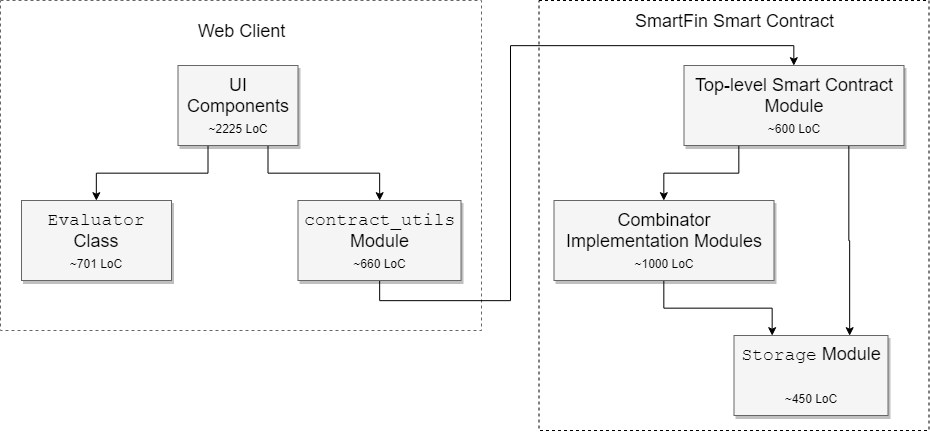
\includegraphics[width=\textwidth]{contributions-block.png}
    \caption{A dependency graph of the modules implemented for this project, with their approximate \textit{Lines of Code} (not including tests).}
    \label{fig:contributions-block}
\end{figure}


\section{Challenges}

\subsubsection{SmartFin Smart Contract Implementation}

Implementing the SmartFin combinator DSL in a smart contract is no small feat; while the number of combinators is relatively limited, representing \textit{any} set of combinators requires a robust generic design when it comes to the implementation of the combinators' semantics and state. Furthermore, this design needed be applicable to \textit{all} combinators, and some are quite unintuitive to represent programmatically. The representation of SmartFin combinators is described in chapter \ref{combinators-main}.

\subsubsection{Ethereum Limitations}

Due to limitations of the Ethereum platform, it is not possible to create a one-to-one representation of a SmartFin contract in smart contract form. Designing solutions to the issues caused by the nature of the Ethereum platform required compromises to be made, and minimising the resulting compromises required designing multiple alternative solutions and evaluating them objectively. Solutions to issues stemming from the Ethereum platform are discussed in chapter \ref{smart-contract-impl}.


\subsubsection{SmartFin Contract Evaluation}

Evaluating SmartFin financial contracts is not a simple problem, even when approaching it in a step-by-step manner, for a couple of reasons. One issue is that SmartFin contracts deal heavily with time, making time an important factor in the evaluation of SmartFin contracts. Keeping track of distinct periods of time based on the SmartFin contract and user interaction was required for step-by-step analysis, requiring a system of describing these time periods to be designed and implemented. Furthermore, keeping track of the current state while requiring the user to enter data can be quite complex, and the ability for the user to revert to any earlier state of step-by-step evaluation can make this even worse. Additionally, the evaluation process requires backtracking for certain combinators, thus resulting in even more complicated behaviour. The implementation of step-by-step evaluation is described in section \ref{client-evaluate}.
\chapter{Background}

\section{Overview}

This chapter describes the background research which has been carried out, with regards to Ethereum and Ethereum smart contracts, the original financial contract DSL, the different ways that SmartFin can be implemented, how observable data can be handled, how the cost of financial contracts written in SmartFin can be evaluated, and how tools for interacting with financial smart contracts can be implemented.


\section{Ethereum, and Smart Contracts}

In order to write a smart contract implementation of SmartFin, it is necessary to understand the inner workings of smart contracts and the platforms which host them.

\subsection{Ethereum}

Ethereum is a platform which hosts a cryptocurrency called \textit{Ether} - this platform uses a custom blockchain (a data structure designed to model an immutable append-only ledger) which is hosted on a distributed set of nodes. Users of the platform have a certain amount of Ether, which acts currency. Ether can be exchanged between users through transactions, which are stored on the blockchain. Ethereum operates similarly to other typical cryptocurrency platforms, like Bitcoin, in this sense\cite{Bitc}. \\

A blockchain consists of several blocks. These blocks contain all of the data in the platform, including any transactions which have taken place. Blocks can only be appended to a blockchain, and existing blocks cannot modified. In order to add new blocks to the blockchain, a number which fulfils specified conditions (a \textit{cryptographic nonce}) must first be found by a node in the system - nodes who search for a nonce are called \textit{miners}. The important detail is that finding a nonce requires a certain amount of work, which is dependent on a \textit{difficulty}. This difficulty can dynamically change to meet the needs of the platform - for example, the difficulty of mining Bitcoin blocks is scaled to modulate the average number of blocks mined in an hour\cite{Bitc}. When a miner discovers a valid nonce, they can create a new block containing any pending transactions and append it to the blockchain\cite{Eth}. In an Ethereum blockchain, a successful miner is rewarded with some Ether - this is one method of introducing new currency into the platform, and encourages mining to occur. If a miner discovers a valid nonce and thus attempts to append a block to the blockchain, all other nodes will validate the block before accepting it as legitimate, thus ensuring that a consensus is reached on the validity of new blocks\cite{Bitc}.

\subsection{Smart Contracts}

Ethereum differs from many other blockchain platforms by also providing a platform upon which special programs (i.e. \textit{smart contracts}) can be run. These programs are also stored on the blockchain, and have functions which can be called by any user of the platform, or by other smart contracts. Smart contracts can also transfer Ether through transactions. \\

Smart contracts typically run on the \textit{Ethereum Virtual Machine}, or \textit{EVM} for short, which runs on many nodes across the network. When a smart contract is run on a node which also creates the next block, the node is reimbursed for the computational resources in \textit{gas} by the account that called the executed function. The gas fee for a contract is an amount of Ether that is proportional with the computational resources used to run the contract; more computationally intense contracts will have higher gas fees. \\

The execution of a smart contract must be deterministic, so that all nodes in the network agree on the outcome of the program's execution - and thus agree on whether any given block is valid. This is not any more efficient than traditional execution, and actually uses \textit{more} resources due to repeated execution of the same program; instead, the benefits of smart contracts include extreme fault-resistance (as only one live node is required to run the program), immutability of any results stored on the blockchain, and a lack of any trusted third-parties\cite{Eth}. \\

The trustless, fault-resistant, immutable nature of smart contracts makes them a great candidate for hosting financial contracts. If the contract required a trusted third-party, then the outcome could be fraudulent if the third-party were biased. If smart contract execution weren't fault-resistant, then there would be no guarantee that any required payments which are possible to fulfil ever actually occur. If the execution were reversible or mutable, then the contracts would become pointless as either party could modify them as desired. \\

Unfortunately, smart contracts are not perfect. A major issue with these programs is that they can often contain hard-to-spot vulnerabilities which can result in smart contracts making unintended transactions, and thus potentially costing the owner large sums of money. These issues are not uncommon - in fact, it was estimated in 2016 that around 45\% of smart contracts contain vulnerabilities\cite{EthSec}. \\

One cause of this issue is that high-level smart contract languages typically provide a complex set of features, including difficult-to-use functionality like iteration and recursion. By giving the developer more freedom to implement complicated smart contract behaviour instead of restricting the use of error-prone features, the risk of introducing errors - like the reentrancy vulnerability demonstrated earlier in listing \ref{listing:reentrancy} - is increased. Even cutting-edge smart contract languages designed with the prevention of common vulnerabilities in mind, like Flint\cite{flint}, still provide a complex feature set and thus can't prevent the introduction of vulnerabilities by human error. \\

This is the main motivator behind the project; allowing financial contract authors to use a restricted yet versatile DSL to write financial contracts and providing a generic smart contract implementation enables contract costs to be evaluated mathematically, and reduces the risk of the financial contract author introducing vulnerabilities or erroneous behaviour.

\subsection{Why Ethereum?}

While Ethereum \textit{does} implement the smart contract functionality required for implementing Smart\-Fin's behaviour, it is not the only platform to do so. Many other platforms also offer some level of smart contract functionality, including Bitcoin\cite{ASC}. One reason for choosing Ethereum is that there exists a large set of development tools available for supporting Ethereum projects - some of which are described in section \ref{dev-tools}. Ethereum also has a large community of users, resulting in a greater volume of documentation compared to other smart contract platforms. The sizeable user-base also means that SmartFin will be useful to more people than if it were implemented on a less popular platform. Besides these factors, Ethereum smart contracts are also more user-friendly than many other platforms (like Bitcoin Script), making the task of implementation less difficult. For all of these reasons, Ethereum makes a good platform for the implementation of SmartFin.

\section{The Design of the Original Combinator DSL for Financial Contracts} \label{DSL-design}

SmartFin, the proposed DSL for financial contracts, is based on a DSL described by Peyton Jones et al.\cite{SPJ}. The design of the original DSL will not be modified significantly, and any modifications are noted clearly in section \ref{DSL-semantics}.

\subsection{Overview} \label{DSL-overview}

The original financial contract DSL is a combinator language used to describe financial contracts. A contract can be represented by a single combinator, or by some composition of combinators. Each financial contract has a \textit{holder}, and a \textit{counter-party}. Typically, the counter-party will be the party making payments, and the holder will be the party receiving payments. \\

A financial contract written in the original DSL can be \textit{acquired} by the holder at any point in time, but the responsibilities of each party may differ depending on when the contract is acquired. For example, consider a contract $C_1$ which requires the counter-party to pay the holder £100 on noon of January 1st 2019 and again on noon of January 1st 2020. $C_1$ requires 2 payments to occur if acquired before 12:00 on 01/01/19, 1 payment to occur if acquired by 12:00 01/01/20, or no payments to occur if acquired after this point. The acquisition date of a contract will therefore affect the responsibilities and thus the value of the contract for each party. \\

A financial contract written in the original DSL may \textit{expire} if no responsibilities outlined in the contract take effect when the contract is acquired after a certain time. For example, the contract $C_1$ has no effect if acquired after 12:00 on 01/01/20. This date is called the \textit{horizon} of the contract. An important thing to note is that a contract's responsibilities could potentially extend past the contract's horizon, but a contract acquired after its horizon will have no effect. \\

Some financial contracts written in the DSL may be dependent on certain parameters. The contract $C_1$, for instance, defines payments of a specific amount on two specific dates. This contract would need to be defined with a constant representing £100, and two date/times. A contract could also be dependent on an variable value, such as the average temperature in London in Celsius, or the distance between two people in metres. Such an objective numeric value is called an \textit{observable}, and can be constant or varying over time. In the original DSL, it is possible to perform arithmetic and functions on observables, values, and dates\cite{SPJ}.

\subsection{Initial Combinators} \label{combinators}

The set of combinators defined in the original DSL is described below, along with each combinator's type signature (described using the notation of Haskell). These combinator definitions originate from Peyton Jones et al.'s paper on the original DSL\cite{SPJ}. The notation used for describing the original DSL is defined in table \ref{dsl-notation}.\\

\begin{table}[ht]
    \begin{center}
        \begin{tabular}{|ll|}
            \hline
            $c, d$ &\textit{Contract} \\
            $o$ &\textit{Observable} \\
            $t$ &\textit{Date/Time} \\
            $k$ &\textit{Currency} \\
            \hline
        \end{tabular}
        \caption{Conventions for the Original DSL's Description}
        \label{dsl-notation}
    \end{center}
\end{table}

\parbox{\textwidth}{
\texttt{zero :: Contract} \\

This combinator represents a contract with no terms. It can be acquired at any time, and thus has no horizon. \\ \\

}

\parbox{\textwidth}{
\texttt{one :: Currency -> Contract} \\

This combinator represents a contract which requires the counter-party to immediately pay the holder one unit of the given currency. This contract can be acquired at any time, and thus has no horizon. \\ \\
}

\parbox{\textwidth}{
\texttt{give :: Contract -> Contract} \\

\texttt{give(c)} represents \texttt{c} with all responsibilities reversed (e.g. if the holder acquires \texttt{give(one(k))}, they must pay the counter-party 1 unit of currency k immediately). The horizon of \texttt{give(c)} is the same as the horizon of \texttt{c}. \\ \\

}

\parbox{\textwidth}{
\texttt{and :: Contract -> Contract -> Contract} \\

When \texttt{and(c, d)} is acquired, both c and d are acquired immediately. Expired sub-contracts are not acquired. \texttt{and(c, d)}'s horizon is the latest of \texttt{c} and \texttt{d}'s horizons. \\ \\
}

\parbox{\textwidth}{
\texttt{or :: Contract -> Contract -> Contract} \\

When \texttt{or(c, d)} is acquired, the holder immediately acquires either c or d. If one has expired, the holder cannot acquire it (and must acquire the other if possible). The horizon of \texttt{or(c, d)} is the latest of \texttt{c} and \texttt{d}'s horizons. \\ \\
}

\parbox{\textwidth}{
\texttt{truncate :: Date -> Contract -> Contract} \\

When \texttt{truncate(t, c)} is acquired, the holder acquires \texttt{c}. The horizon of \texttt{truncate(t, c)} is the earliest of \texttt{t} and the horizon of \texttt{c} (thus \texttt{truncate(t, c)} cannot be acquired after either horizon has passed). \\ \\
}

\parbox{\textwidth}{
\texttt{then :: Contract -> Contract -> Contract} \\

When acquiring \texttt{then(c, d)}, the holder acquires \texttt{c} if \texttt{c} has not expired, or \texttt{d} if \texttt{c} has expired and \texttt{d} has not. \texttt{then(c, d)}'s horizon is the latest of \texttt{c} and \texttt{d}'s horizons. \\ \\
}

\parbox{\textwidth}{
\texttt{scale :: Observable -> Contract -> Contract} \\

\texttt{scale(o, c)} represents \texttt{c} with all payments multiplied by the value of the observable \texttt{o} at the time of acquisition. \texttt{scale(o, c)} has the same horizon as \texttt{c}. \\ \\
}

\parbox{\textwidth}{
\texttt{get :: Contract -> Contract} \\

After the holder acquires \texttt{get(c)}, \texttt{c} is acquired at the moment in time when the horizon of \texttt{c} is reached. \texttt{get(c)} has the same horizon as \texttt{c}. \\ \\
}

\parbox{\textwidth}{
\texttt{anytime :: Contract -> Contract} \\

After \texttt{anytime(c)} is acquired, \texttt{c} must be acquired by the holder at any point before it expires. The holder can decide when to acquire \texttt{c}. \texttt{anytime(c)} has the same horizon as \texttt{c}.
}


\subsection{Example Financial Contracts in the Original DSL} \label{example-contracts}

\subsubsection{European Option}

A European option allows the holder to choose, on a particular date, between acquiring an underlying contract or acquiring nothing. A European option allowing the holder to choose between receiving £500 GBP from the counter-party, and receiving/paying nothing, at midnight on the 1st of January 2020 is defined as follows:

\begin{Verbatim}[frame=single, samepage=true, rulecolor=\textcolor{black!50}]
get(truncate(<01/01/2020, 00:00:00>, or(
    scale(500, one(GBP)),
    zero
)))
\end{Verbatim}

The \texttt{get} combinator, if acquired, causes the sub-contract to be acquired at its horizon. This means that \texttt{truncate(<01/01/2020 00:00:00>, or(scale(500, one(GBP)), zero))} is acquired at 00\-:00:00 on 01/01/2020, as the \texttt{truncate} combinator sets the sub-contract's horizon to this time. \\

The \texttt{or} combinator is thus acquired at midnight on the 1st of January 2020, as long as the contract is acquired before this. This enables the holder to choose to acquire one of the two sub-contracts at this time. The first sub-contract is \texttt{scale(500, one(GBP))}. The \texttt{one(GBP)} combinator requires the counter-party to pay the holder £1 upon acquisition, and the \texttt{scale(500...} combinator multiplies this by £500, thus this sub-contract requires the counter-party to pay the holder £500 in total upon acquisition. The second sub-contract, \texttt{zero}, requires neither the holder nor the counter-party to pay anything. As such, the holder can choose between being paid £500 or £0 at this time.


\subsubsection{Simple Loan with Variable Repayment}

Take a contract which can only be acquired before 00:00:00 on 01/01/2020, and allows the holder to obtain £1 upon acquisition, and then either pay back £2 by 00:00:00 on 01/02/2020, or pay back £3 after 00:00:00 on 01/02/2020 and before 00:00:00 on 01/03/2020. The holder \textit{must} pay one of these amounts by 00:00:00 on 01/03/2020. This contract is defined is follows:

\begin{Verbatim}[frame=single, samepage=true, rulecolor=\textcolor{black!50}]
truncate(<01/01/2020 00:00:00>, and(
    one(GBP),
    anytime(then(
        truncate(<01/02/2020 00:00:00>, give(scale(2, one(GBP)))),
        truncate(<01/03/2020 00:00:00>, give(scale(3, one(GBP))))
    ))
))
\end{Verbatim}


The first \texttt{truncate} combinator causes the contract to expire at the given date. The \texttt{and} combinator acquires both sub-contracts when acquired, i.e. \texttt{one(GBP)} and \texttt{anytime(...)}. \texttt{one(GBP)} requires the counter-party to pay the holder £1 on acquisition. The \texttt{anytime} combinator allows the holder to choose when to acquire the sub-contract once acquired, but the sub-contract must be acquired before its horizon is passed and it expires. The \texttt{then} combinator acquires its first sub-contract if it hasn't expired, otherwise it acquires the second sub-combinator. If the \texttt{anytime} sub-contract is acquired before 00:00:00 on 01/02/2020, then the \texttt{then} combinator acquires the first sub-contract, which requires the holder to pay the counter-party £2 immediately due to \texttt{give} and \texttt{scale}. If the \texttt{anytime} sub-contract is acquired after this point, then the second \texttt{then} sub-contract is acquired, requiring the holder to pay the counter-party \texttt{£3} immediately. The \texttt{anytime} sub-contract must be acquired before the \texttt{then} combinator expires, at 00:00:00 on 01/03/2020.


\subsection{Representing Financial Contracts}

In order to correctly design the full set of combinators for SmartFin, it is important to consider how SmartFin financial contracts will be represented in a smart contract implementation. \\

One way of representing these SmartFin contracts in a smart contract implementation is to use a functional approach. This involves creating a function representing each combinator, and having the functions carry out the actions which would occur when their respective combinator is acquired. This follows the description of the original DSL quite closely; however, due to the inherent statefulness required in these financial contracts (including state like time of acquisition, values of observables, etc), a functional approach is very difficult to implement. This is especially true as the state must be stored on the blockchain over a period of time between interactions with the smart contract. While a functional approach is possible, it would require workarounds to store combinators' state persistently - thus suggesting that this approach is not the best method of implementation. \\

SmartFin contracts can also be represented as structs where each combinator is represented by an object. For example, in the original DSL the contract defined as \texttt{scale(5, one())} would be represented by an object representing \texttt{scale} which acquires its sub-object with 5 times the value, containing an object representing \texttt{one} which causes the counter-party to pay the holder 1 Ether at the time of acquisition. By using objects instead of functions, the issue of storing the state of each combinator can be solved trivially while still maintaining the compositional nature of combinators.


\subsection{Difficult Combinators}

Certain combinators of the original DSL described in \ref{combinators} are difficult to represent directly in a smart contract environment. The \texttt{get} combinator acquires the sub-contract at its horizon, i.e. as late as possible before expiration. This is difficult to represent as callbacks cannot be scheduled in Ethereum smart contracts due to the necessity of deterministic evaluation on all nodes in the network, and thus a sub-contract cannot be automatically acquired at a given time. \\

Another problematic combinator is the \texttt{anytime} combinator. When acquired, this combinator requires the holder to acquire its sub-contract before the sub-contract expires. This is difficult to represent as there is no way to force the holder to acquire a contract (i.e. call an acquire function) in a given time-frame, or ever, from a smart contract. These issues will require further consideration when implementing SmartFin's smart contract implementation, and may require some compromises to be made.


\subsection{Payment}

\subsubsection{Scheduled Payments}

As described previously, time-based callbacks cannot be registered directly within an Ethereum smart contract to ensure determinism. This means that a smart contract cannot pay a user automatically at a given time, and so a financial contract which states that party A must pay party B at a given time is not able to be represented directly as a smart contract. It is possible to call a function on a smart contract at a given time through some external tool, but this effectively requires a trusted third-party (in the form of whoever is executing this tool). This is an issue which must be considered when implementing SmartFin's smart contract behaviour.

\subsubsection{Exhaustion of Funds} \label{fund-exhaustion}

In the real world, if a financial contract exists between two parties, then any party which fails to fulfil their responsibilities as laid out in the contract can be sued for reparations. In the world of smart contracts, there is no such guarantee. If party A acquires a smart contract which says that party B will pay them some sum of money, party B must provide that money to the smart contract before payment can occur. If a smart contract does not have enough funds to fulfil all payments, there is nothing that party A can do to mitigate this issue (unless the smart contract is backed by some real-world legally binding contract). This also requires compromises to be made when implementing SmartFin's smart contract behaviour.


\subsection{Handling Observables} \label{dsl-observables}

The original DSL can make use of external data in the form of \textit{observables}. This allows a financial contract's value to be modified based on external numerical data.

\subsubsection{Defining Observables}

The smart contract implementation of SmartFin needs some way of defining observables' values. This is needed because the smart contract needs to know the values of each observable in order to calculate the value of payments, and so it needs to allow some way of obtaining/setting the value of each observable. \\

It could be useful to allow some other constraints to be set on observables; for example, if a financial smart contract pays out some value depending on an unbounded observable, there will be no guarantee on how much Ether must be provided for all payments to be fulfilled, and evaluation of the underlying SmartFin contract may not give a concrete value. This suggests that providing a bound for some observables may be useful for both guaranteeing payment and making evaluation of the SmartFin contract more useful.

\subsubsection{Passing External Data to the Contract}

Unfortunately, it is not possible for smart contracts to read data directly from an external server. This is because it could introduce non-deterministic execution to the EVM (i.e. two nodes executing the contract in different places could receive different data from the same address). This means that observables cannot be dynamically updated in the smart contract implementation of SmartFin. \\

Instead of dynamically reading data from an external source, observable values can be passed in through a function call. This can be done by defining a trusted source in the SmartFin contract definition, or by requiring the holder and counter-party to agree on a value (this more closely matches the original definition of an observable\cite{SPJ}); the latter system could be implemented through a signature-based system, or by storing suggested observable values of each party.


\section{Development Tools} \label{dev-tools}

In order to implement a smart contract representation of SmartFin's behaviour, a tool-set is needed for development and testing. There are several different toolchains which could be used for this, which are discussed and evaluated in this section. As smart contracts can be used to deal with real funds, any errors could potentially have a large real-world cost; as such, a testing framework will be a necessity to provide some basic evidence of correctness.


\subsubsection{Local Ethereum Network}

Ethereum allows developers to deploy their own local Ethereum blockchains, for testing purposes. These blockchains act like the default Ethereum blockchain, although they have several parameters which can be customised. Smart contracts can be hosted on these blockchains for testing purposes. \\

Parameters of the Ethereum network which can be modified include the difficulty of mining a block, the maximum limit a smart contract can cost to execute (in gas), the minimum gas a miner will accept, and a set of accounts to have Ether pre-allocated to them upon the creation of the blockchain. This allows the writing of arbitrarily complex contracts, the mining of blocks quickly and cheaply, and the ability to obtain Ether immediately - all of which are useful for testing contracts\cite{Geth}. \\

Setting up a bespoke blockchain just for testing smart contracts is quite complicated. There are many options for which values must be chosen, and not a huge number of resources which explain which option does what. This also only really provides the ability to manually test smart contracts through an Ethereum client, and does not provide any resources for automated testing (although external tools to do this do exist). It is still a useful option where public blockchains are not appropriate, however, and several clients allow easier set-up.


\subsubsection{Truffle Toolchain}

Another way that smart contracts can be tested is by using the Truffle toolchain. Truffle provides tools for running a local blockchain, smart contract compilation/deployment, automated testing, console interaction with contracts, build pipelines, and more\cite{Truffle}. The main tool that is needed for this project is an automated testing framework, which Truffle provides. \\

By using Truffle for automated testing, some continuous-integration can be put into place on the DSL. This enables rapid iteration of different smart contract functionality with lower risk of breaking existing features or introducing bugs. For these reasons (as well as ease-of-use), Truffle is a good option for the project's development toolchain.


\subsubsection{Remix}

Remix is an online IDE for writing smart contracts in Solidity. It provides tools for writing, compiling, testing, debugging, and deploying smart contracts\cite{REMIX}. Smart contracts written in Remix can be deployed to a blockchain of the user's choosing (either public or local). Function calls can then be made to the contract from the IDE, including payable functions (if authorised by some Ethereum account manager like MetaMask). It is also possible to define unit tests and run them from Remix, or from the command line\cite{RMXTST}. This IDE can be a useful tool if any part of development requires the creation of smart contracts in Solidity.


\subsubsection{Parity Tools} \label{parity-tools}

Parity Technologies provide a set of tools for developing smart contracts in Rust which compile to WebAssembly (\textit{wasm}), including a set of Rust modules for interacting with Ethereum\cite{parity-technologies}. These modules include:

\begin{itemize}
    \item \texttt{pwasm-ethereum}: A module with bindings for interacting with an Ethereum blockchain, implementing functions like \texttt{sender} to obtain the sender of a function call transaction, and \texttt{call} to create and send a transaction\cite{pwasm-ethereum}.
    \item \texttt{pwasm-std}: A module implementing some features of the Rust standard library, which is incompatible with the \texttt{pwasm} modules\cite{pwasm-std}.
    \item \texttt{pwasm-abi}: A module which provides macros for deriving a smart contract ABI (the smart-contract equivalent of an API) from a Rust trait, with annotations like \texttt{payable}, which indicates that a call transaction for the described function may contain Ether\cite{pwasm-abi}.
    \item \texttt{pwasm-test}: A module which provides mocking functionality for \texttt{pwasm-ethereum} function calls, to be used with automated testing\cite{pwasm-test}. \\
\end{itemize}

They also provide the Parity blockchain client, which is a configurable client that can run a private blockchain capable of hosting wasm smart contracts (which not all blockchain clients are able to do)\cite{pwasm-client-wasm}. These tools make it possible to implement a smart contract representation of SmartFin's behaviour in Rust, which may be a good option due to the relatively thorough documentation available for Rust in comparison to many smart contract languages.


\subsubsection{Web3.js}

Web3.js is a JavaScript package containing a collection of libraries for interacting with the Ethereum API\cite{web3-intro}. This can be useful for deploying and interacting with smart contracts, and implementing integration tests (in conjunction with a testing framework). This package is also a useful option for implementing the external tool which deploys/interacts with financial smart contracts.


\subsubsection{MetaMask}

MetaMask is a browser extension which allows the user to authorise Ethereum transactions on a blockchain (either public or private) securely\cite{MMSK}. This enables manual testing of smart contracts, which is a valuable tool when testing Ethereum smart contracts written in any language. MetaMask is also a good option for connecting to a desired blockchain, and for deploying and interacting with financial smart contracts, from the external tool.


\section{SmartFin Smart Contract Implementation} \label{DSL-implementation-technologies}

There are numerous design choices to be made with regards to the smart contract implementation of SmartFin. An important design choice is the form that SmartFin is implemented in; there are several major options, including:
\begin{itemize}
    \item Creating a SmartFin library for an existing smart contract language, which can be called from smart contracts written by anyone.
    \item Writing a smart contract which implements SmartFin's behaviour, and passing it a SmartFin contract definition.
    \item Creating a bespoke compiler for SmartFin which can compile SmartFin financial contracts to smart contracts. \\
\end{itemize}

There are several pros and cons to each of these choices, which are analysed in this section before a conclusion is reached on which method is most appropriate.

\subsection{Creating a Library for an Existing Smart Contract Language}

One way to implement SmartFin is to write a package for an existing smart contract language (like Solidity), and allow the user to call the required functions. With this method, the user can write a smart contract which calls into the relevant library functions for their SmartFin contract.

\subsubsection{Solidity Libraries}

Solidity, a high-level smart contract language for Ethereum, allows the writing and deployment of special smart contracts called \textit{libraries}. Libraries are smart contracts which are deployed only once, and define functions which which will be run in the calling smart contract's context\cite{EthLib}. This allows developers to define reusable functions in a single deployed library, and call said functions from any smart contract on the same blockchain. \\

Using Solidity's library functionality, it is possible to implement SmartFin's combinators as functions or structs in a library, thus allowing developers to access them from any smart contract they write - as long as the library is committed to the same blockchain. \\

This approach does not require implementing any compilation step to obtain a smart contract, making implementation more straightforward. The smart contracts which use a library would also be smaller in size compared to a smart contract which takes a SmartFin contract in the constructor, which would need to include all of the combinators' logic. This would reduce the amount of gas (Ether spent on transaction fees) required to deploy financial smart contracts. \\

One requirement of this approach is that the user must write a smart contract which calls these library functions. Unfortunately, this is problematic for a few reasons; firstly, these smart contracts can have code added which modifies the behaviour of the smart contract separately from the SmartFin contract. For example, before calling functions from the SmartFin library, a smart contract could immediately pay 1 Ether to the address of the counter-party. While this could be useful in specific situations, it clearly changes the value of the smart contract in a way unrelated to the SmartFin library calls, thus making it much more difficult to analyse. This level of freedom increases the risk of making unintended payments, whereas other methods of implementing SmartFin where a financial smart contract is output from a compiler or passed a SmartFin contract would not be affected by this problem, as the developer would not be expected to modify the smart contract directly. \\

Another problem with this solution is that it requires developers to understand both SmartFin and Solidity in order to create financial smart contracts. This adds a barrier to entry, and also increases the possibility of introducing errors which unintentionally affect the value of the financial smart contract. \\

A third issue is that analysing the value of a smart contract which calls functions from a library is difficult, as it requires analysing the smart contract to extract the definition of the SmartFin contract from within. This could be solved by requiring the developer to define the SmartFin contract inside the smart contract, and separately pass it into the analysis tool. This is not ideal as it may increase the risk of errors occurring; for example a developer may update their smart contract code but not the SmartFin contract passed into the analysis tool, thus receiving an inaccurate evaluation of the SmartFin contract.

\subsubsection{EthPM - The Ethereum Package Management System}

Another method of defining a set of structs and functions for representing SmartFin in Ethereum smart contracts is the use of EthPM, a package management system built for Ethereum. EthPM packages can include smart contract code, and the addresses of deployed smart contracts\cite{EthPM}. The SmartFin DSL can be implemented as a set of functions or structs which are included in the EthPM package, and accessed from smart contracts which depend on it. EthPM would then handle the building of the final financial smart contract. \\

This unfortunately suffers from many of the same issues as writing a typical Solidity library. The user is still required to write a smart contract which calls the SmartFin functions, potentially introducing erroneous behaviour while doing so. The benefit of simpler redistribution of the package is also rendered slightly moot, as external tools for interacting with or analysing the value of a SmartFin contract cannot be distributed in an EthPM package, so another route of distribution will be needed either way. The added value of a package manager is also somewhat futile, as financial smart contracts should ideally have no other functionality besides the SmartFin function calls and thus shouldn't need to import any other packages.


\subsection{Passing a SmartFin Contract to a Smart Contract} \label{traditional-dsl}

Instead of allowing the user to write their own smart contract code which calls into some SmartFin module, another option is to allow the user to write their SmartFin contract and pass it to a pre-written smart contract which implements the behaviour for any SmartFin contract definition. For this approach, the smart contract implementing SmartFin's behaviour can be written in any language which can compile to a smart contract. \\

One benefit of this method is that the end user only needs to implement a SmartFin contract, and \textit{no} smart contract implementation. This lowers the barrier to entry for creating financial smart contracts, as the user only needs to learn how to use SmartFin, as opposed to an entire smart contract language like Solidity. This method also means that obtaining the SmartFin contract for analysis/evaluation is simple, as this contract can be defined separately from the smart contract implementation. \\

Additionally, passing the SmartFin contract to a pre-written smart contract prevents the user from modifying the final value of the smart contract by writing smart contract code outside of the SmartFin contract definition, as the user only writes their SmartFin contract and never touches the smart contract. Another benefit is that very little implementation work needs to be done from a compilation point of view, as the existing compilers for the high-level language used to implement SmartFin should handle the final compilation to a smart contract.


\subsubsection{Implementing with a Traditional Smart Contract Language}

Similarly to the implementation of SmartFin's behaviour as a Solidity library discussed earlier, the smart contract that implements SmartFin's behaviour can be written in Solidity (or another smart contract language). This smart contract can take and parse the SmartFin contract definition in the constructor, and then set its state so that its behaviour matches that of the given SmartFin contract.


\subsubsection{Implementing with a Traditional High-Level Language}

Instead of implementing SmartFin's behaviour in Solidity, it can also be implemented in some language which compiles to WebAssembly\cite{EWASMDOC}; WebAssembly is typically more efficient than Solidity for numerous reasons - like the use of 256 bit integers in Solidity\cite{FASEVM} - and it is being supported by W3C, a group consisting of multiple member corporations including Google and Mozilla\cite{W3CMEM}, whereas Solidity is only supported by the Ethereum foundation. The ability to use tried-and-tested high-level languages would also be helpful, as they typically have more plentiful documentation and a more polished approach to language design compared to the relatively-new smart contract languages. \\

The main issue with this method is that producing a WebAssembly smart contract from a high-level language is not necessarily straightforward, as some functionality from the high-level language is often not usable on the Ethereum platform. This can make the implementation of SmartFin's behaviour more difficult. The main features absent in ewasm are related to non-determinism\cite{EWASMDOC}, which shouldn't cause many issues with the implementation of SmartFin's behaviour which would not be present in all smart contract languages, so this should not be a major problem with regards to this specific method of implementation. \\

There are a few high-level languages which can be compiled to WebAssembly, but most of them are not viable for this project. Haskell has numerous ongoing WebAssembly compilation tools in development, but there are none which are implemented beyond the alpha stage\cite{DHC}\cite{ASTR}. Scala is in a similar situation, with an underdeveloped wasm tool-set\cite{SCWASM}. Kotlin, Lua, Python, and TypeScript can all compile to WebAssembly, but do not provide tools for implementing Ethereum functionality like sending and receiving transactions\cite{AWASM}. \\

Rust\cite{rust}, on the other hand, has a set of tools released by Parity Technologies for compiling Rust programs to ewasm smart contracts\cite{PWASM}, as previously described in section \ref{parity-tools}. These tools include bindings for Rust programs to interact with an Ethereum blockchain, alternative implementations of standard-library features which are incompatible with ewasm, tools for compiling smart contracts from Rust, tools for testing Rust smart contracts, and even a configurable blockchain client which can run these contracts. As such, Rust is a suitable high-level language to use to implement the smart contract which can represent any given SmartFin contract.


\subsection{Creating a Bespoke Language and Compiling to a Low-Level Language}

Instead of implementing a smart contract which represents the behaviour of any given SmartFin contract in a high-level language, SmartFin contracts could be compiled directly to low-level smart contract code (wasm, Yul\cite{yul}, or similar) by implementing a bespoke compiler. Similarly to implementing SmartFin's behaviour in a high-level language, this method also only requires users to define their SmartFin contract, with all of the same benefits. \\

The main practical change between this method and the method described in \ref{traditional-dsl} is that Smart\-Fin's behaviour is implemented in a low-level language; this allows the implementation of SmartFin to use all of the available functionality, which may not be possible if compiling from a high-level language. This could allow improvements to SmartFin's functionality which would not otherwise be possible. \\

The biggest problem with this method is that while implementing SmartFin in a low-level smart contract language may result in a more optimal implementation than the higher-level approach, it is much more difficult to write. Under the assumption that high-level languages have well-optimised compilers for producing low-level smart contract code, then the performance gains may not even be significant. Furthermore, if financial smart contracts are used within financial institutions then it is likely that the blockchain they are deployed to will not handle gas in the traditional manner, and would be more likely to have no gas payments, further reducing the benefits to improved performance. In these cases, implementing a compiler to compile SmartFin contracts to low-level smart contract code may only add to the effort required with little benefit.


\subsection{SmartFin Implementation Summary}

Overall, the problems with implementing SmartFin with a Solidity library directly affect the end user, making financial smart contracts more difficult to create, and making it easier to unintentionally alter the smart contract's value. As such, a Solidity library/package is an unsuitable choice for implementing SmartFin. \\

Implementing SmartFin's behaviour in a high-level language or compiling from SmartFin to low-level smart contract code mitigates these two issues. Implementing SmartFin compilation \textit{may} offer performance benefits, whereas high-level languages may be less difficult to work with; the performance benefits from low-level languages are also not guaranteed, and dubious in their utility. As such, the difficulty of implementing compilation to low-level contract code outweighs any expected benefits, and implementing in a high-level language which compiles to WebAssembly is the more suitable option.


\section{External Tool for Financial Smart Contract Interaction}

In order to compose and evaluate financial contracts written in SmartFin, and to deploy and interact with their smart contract representations, an external tool is needed. As discussed in section \ref{dev-tools}, there are several browser-based tools which facilitate interaction with Ethereum blockchains, namely MetaMask and Web3.js. Thanks to these tools, implementing a web client to handle these external functions is a viable solution. \\

While other languages provide tools for interacting with Ethereum blockchains (like the Python implementation of Web3\cite{web3-py}), the large swathe of support for blockchain interaction in the browser makes a web client a very attractive option. Package management tools like Yarn\cite{yarn}, graphical frameworks like React\cite{react}, and testing frameworks like Mocha\cite{mocha} can also aid rapid development of the web client. Furthermore, MetaMask provides an easy to use and secure method of connecting to the blockchain, and it is only available as a browser extension\cite{MMSK}. As such, implementing the external tool as a web client is a valid solution which enables rapid development and has few obvious issues.


\section{SmartFin Contract Cost Analysis} \label{cost-analysis}

A useful feature provided through the external tool is the mathematical evaluation of a given SmartFin contract's potential cost/value with any given acquisition times. This is particularly useful to prevent the writing of SmartFin contracts with unexpected behaviour. The mathematical implementation of such a tool for the original DSL is outlined in the paper by Peyton Jones et al.\cite{SPJ}. \\

The value of each contract is dependent on its sub-contracts. For example, in the original DSL the contract \texttt{and(one(GBP), one(GBP))} will have a value of $(£1 + £1) = £2$, thus the value of an \texttt{and} combinator is equal to the sum of its sub-contracts' values. This makes the general approach behind contract evaluation fairly straightforward, where the contract is treated as a tree with the top-level contract as the root, and all sub-contracts as children. The tree can be traversed depth-first, and then backtracked to the root while accumulating the required values. \\

There are other evaluation issues that the paper by Peyton Jones et al.\cite{SPJ} deals with, such as inflation rates and exchange rates. Because this project is concerned with a smart contract implementation of SmartFin, financial smart contracts will only deal in the relevant cryptocurrency (Ether), and thus evaluation based on exchange rates of payments is slightly irrelevant. The use of Ether also makes the analysis of inflation quite difficult, as cryptocurrencies are notoriously volatile in value. These two features are therefore less useful (albeit not useless) and require significant work to implement; as such, they are not an essential feature for the analysis of SmartFin contracts. \\

One potential issue with the evaluation of SmartFin contracts is the presence of observables; in order to obtain a value of a SmartFin contract with a given acquisition time, the value of any observables must be evaluated. This is a difficult problem to solve, as modelling the value of observables requires allowing users to input some representation of a numerical model representing this value over time, and the implementation of algorithms to evaluate these models. This is a huge undertaking, and as such a more basic evaluation mechanism which does not estimate the value of observables is a more viable option given the time constraints.


\section{Remarks}

After significant background research, certain conclusions can be reached with regards to the approaches taken for this project. In order to represent SmartFin contracts as financial smart contracts, Ethereum is the most viable smart contract platform due to its sizeable user-base, the vast set of development tools available, and the platform's user-friendly nature. \\

A smart contract representation of SmartFin can generally follow the intended financial contract behaviour accurately, but certain issues may arise. Scheduling of payments is effectively impossible due to the distributed and deterministic nature of Ethereum blockchains, where scheduled callbacks are impossible without requiring external interaction. Exhaustion of funds is also a problem which may occur with financial smart contracts, as there is no way for a smart contract to ensure that a user pays the amount required by the contract definition. Observable values will also be impossible to obtain dynamically due to the deterministic nature of the blockchain, and thus they will need to be passed to the contract in some way. These issues must all be dealt with when implementing a smart contract representation of SmartFin. \\

When developing the smart contract implementation of SmartFin, allowing the SmartFin contract definition to be passed through the constructor is a beneficial approach as it prevents the user from altering the smart contract's behaviour directly, and makes analysis of the SmartFin contract easy. Compiling directly from the SmartFin contract to a low-level smart contract is comparatively very difficult to implement for little gain, and requiring the user to write a smart contract which calls into a SmartFin library would make analysis difficult and risk the introduction of errors. Implementing the smart contract representation of SmartFin in Rust/wasm ensures long term support from the W3C group, and improved performance compared to Solidity and other smart contract languages - as such, it is the option of choice. \\

In order to implement the external tool for evaluating SmartFin contracts and deploying or interacting with financial smart contracts, a web client makes a lot of sense. This is because of the multitude of web-development tools available, and the existence of various modules/extensions for communicating between a blockchain and a web client. These factors ensure that development of the web client can be rapid and problem-free, and that the external tool can carry out all of the required functionality. \\

The following chapters will describe the design of the SmartFin DSL, the smart contract implementation of SmartFin and its combinators, and the web client used to interact with financial smart contracts.

% \chapter{Plan}

\section{Overview}

The implementation of the financial smart contract DSL and analysis tool can be broken up into several steps. The general design of the internal representation of financial smart contracts has been carried out in section \ref{DSL-design} (although this may be tweaked in future)\todo{Shouldn't be in background}. This design needs to be implemented in a high-level language, likely Rust, and to have the functionality of all combinators described in section \ref{combinators} implemented. The DSL functionality must also be tested thoroughly with unit and integration tests. The analysis tool should also be implemented, allowing the evaluation of a financial contract's value at a given point in time, and tested with unit tests. There are a few extra features which can be added to the DSL/analysis tool as extensions, if time permits. The project report must also be produced once major development is complete.

\section{DSL Implementation} \label{DSL-implentation-timeframe}

The major steps for implementing the DSL and compilation process are:
\begin{enumerate}
    \item Implementing very basic smart contracts in a high-level language, compiling them to WebAssembly, and deploying/testing on a blockchain (to nail down the toolchain).
    \item Implementing the basic generic structure of the DSL in Rust (as described in section \ref{DSL-design}).
    \item Implementing generic parsing/compilation functionality for financial smart contracts.
    \item Implementing the \texttt{zero} combinator in Rust, and testing it (via manual and unit testing).
    \item Implementing the \texttt{one} combinator in Rust (thus handling payment), and testing it.
    \item Implementing other basic combinators (\texttt{and}, \texttt{or}, \texttt{then}) and testing them.
    \item Implementing and testing the more complicated combinators one at a time (\texttt{scale}, \texttt{truncate}, \texttt{give}, \texttt{get}, and \texttt{anytime}).
\end{enumerate}

In the ideal case, the implementation of the DSL will be completed by the 19th of April. This will allow me to split my time evenly between the implementation of the DSL, and the implementation of the analysis tool. In the worst case scenario, the time taken for the completion of the DSL could extend until the 29th of April, although this will limit the amount of time spent on the analysis tool and report (and any extensions attempted). The steps up to and including step 5 should ideally be completed by the 29th of March, leaving the 30th of March to the 19th of April open for the implementation of most of the combinators - approximately balancing the time given to each of these two sets of steps, when accounting for limited available time during spring term.


\section{Analysis Tool Implementation}

The major steps for implementing the analysis tool in the order of implementation are as follows:
\begin{enumerate}
    \item Implementing a basic parser for the DSL (or re-purposing the parser used for compiling the smart contract), and tests.
    \item Implementing the general evaluation pipeline - converting input to suitable data structure, traversal and memoisation - and tests.
    \item Implementing evaluation rules for simple combinators (\texttt{zero}, \texttt{one}), and tests.
    \item Implementing evaluation rules for the remaining combinators, and tests.
\end{enumerate}

If the ideal time frame of completion of the steps outlined in section \ref{DSL-implentation-timeframe} is kept to, then the implementation of steps in this section should begin on the 19th of April. Ideally, these features should all be implemented by the 17th of May. This splits the amount of time given to the implementation of the DSL and the analysis tool evenly (given the limited available time during spring term), and leaves a month for the writing of the final report. The implementation of the analysis tool should not take as long as the DSL, as the major details behind the evaluation process are described in \cite{SPJ} (whereas the implementation of the DSL was only described in hypothetical terms). I would estimate that the implementation of the analysis tool could be completed by some time around the 6th of May, leaving some time available to work on an extension. If the DSL implementation overruns until the 29th of April, then the analysis tool should be completed by around the 16th of May still (leaving no time for extensions). In the worst case scenario, finishing the analysis tool by the 24th of May should leave 3.5 weeks for the final report, which is still an ample amount of time.


\section{Final Report}

The final report will need to be completed by the 17th of June. The major parts of the discussion of implementation details in the final report should ideally be written while the DSL and analysis tool are being implemented, although likely in shorthand. Given this, the majority of the time working on the report will be spent writing up these notes, and writing the evaluation, conclusion, and user guide (which will be necessary for the usage of the DSL and analysis tool). I would estimate that this work should take around 1 month to complete, without rushing, thus the implementation of the analysis tool and any extensions should be completed by the 17th of May. If necessary, the report could probably be finished in around 3 weeks, although this may affect the quality of the report.

\section{Extensions}

The analysis tool should be completed by the 17th of May, but it may be finished before this deadline. During the time between completion of the analysis tool and the writing of the final report, there may be time to implement some extensions to the project. It may also be possible to work on these extensions if the final report is finished before the deadline, although this time may be better spent polishing the report. Possible extensions for this project include the modelling of inflation and exchange rates in the analysis tool (as described in section \ref{cost-analysis}), the improvement of how fund exhaustion is handled (see section \ref{fund-exhaustion}), the implementation of new combinators (whether for conciseness or utility), the implementation of bounding for the values of observables (see section \ref{dsl-observables}), developing a GUI for the analysis tool, and outputting graphs of a contract's value over time from the analysis tool.
\chapter{The Design of SmartFin} \label{combinator-DSL}

The main goal of this project is to provide a smart contract implementation of a DSL for financial contracts. Before discussing this implementation, this chapter defines the syntax and semantics of the DSL being implemented, SmartFin. \\

The syntax and semantics of SmartFin are derived from a DSL proposed by Peyton Jones et al.\cite{SPJ}, described in section \ref{DSL-design}, but SmartFin varies slightly from this original DSL. The smart contract implementing SmartFin must behave correctly when any SmartFin contract definition is provided, according to the syntax and semantics laid out in this chapter.


\section{Overview of SmartFin Financial Contracts}

SmartFin is a combinator domain-specific language used to describe financial contracts, and in general operates very similarly to the DSL defined by Peyton Jones et al.\cite{SPJ} which is described in section \ref{DSL-overview}. The general gist is that a SmartFin contract represents a financial contract between two parties, which can define payments between these parties. The \textit{holder} party is able to acquire a SmartFin contract - just as a traditional financial contract would be signed - and any obligations are carried out subsequently. SmartFin contracts can expire, and contracts can rely on external input.


\section{Syntax} \label{DSL-BNF}

The syntax of SmartFin is very simple, due to its combinatorial nature. The Backus-Naur form of the grammar is as follows, where \texttt{<name>} is a string starting with a non-integer character, \texttt{<time>} is a date and time, \texttt{<integer>} is an integer value, and \texttt{<address>} is an Ethereum address: \\

\setlength{\grammarindent}{10em}
\begin{grammar}
<contract> ::= `zero'
\alt `one'
\alt `give' <contract>
\alt `get' <contract>
\alt `anytime' <contract>
\alt `scale' <observable> <contract>
\alt `truncate' <time> <contract>
\alt `and' <contract> <contract>
\alt `or' <contract> <contract>
\alt `then' <contract> <contract>

<observable> ::= <integer> | <name> <address>
\end{grammar}

This syntax has one major difference from the syntax of the original DSL presented in the paper by Peyton Jones et al.\cite{SPJ}. This difference is the representation of \textit{observables}, used with the \texttt{scale} combinator in the \texttt{<contract>} rule. In the original DSL, an \texttt{observable} takes a constant value, or a representation of a time-varying value, but its syntax was left abstract due to the somewhat abstract nature of the combinators' implementation in the paper. The paper was more focused on evaluating financial contracts written in this form than representing them programmatically. As this project requires a concrete implementation of the DSL, the syntax cannot be left abstract. Because of this, it is necessary to give a specific definition of an observable's syntax; the chosen definition being a constant integer value, or a name and an Ethereum address. The purpose of these representations is explained further in section \ref{DSL-semantics}. The original DSL also allowed observables to have mathematical operations carried out on them, whereas SmartFin does not. \\

For clarity, the format of the \texttt{<time>} rule in the provided BNF can be either UNIX Epoch time, or a date and time in the format \texttt{"<DD/MM/YYYY HH:mm:ss +ZZ>"} - where \texttt{"DD"} is a two-digit date, \texttt{"MM"} is a two-digit month, \texttt{"YYYY"} is a four-digit year, \texttt{"HH"} is a two-digit hour, \texttt{"mm"} is a two-digit minute, \texttt{"ss"} is a two-digit second, and \texttt{"+ZZ"} is an optional positive or negative two-digit time zone offset.


\section{Semantics} \label{DSL-semantics}

Each combinator has a specific meaning, potentially depending on sub-combinators, times, and/or observables. This section gives a definition of the semantics of SmartFin combinators where they differ from the original DSL, namely \texttt{one} and \texttt{scale}. For combinators not listed here, see \ref{combinators} for their semantics. The conventions used to represent the syntax of these combinators is defined in figure \ref{combinator-semantics-notation}, and the definition of each combinator's semantics is as follows: \\

\begin{table}[ht]
    \begin{center}
        \begin{tabular}{|ll|}
            \hline
            $c, d$ &\textit{Contract} \\
            $o$ &\textit{Observable} \\
            $x$ &\textit{Constant Value} \\
            $n$ &\textit{Observable Name (as in section \ref{DSL-BNF})} \\
            $a$ &\textit{Ethereum Address} \\
            $t$ &\textit{Time} \\
            \hline
        \end{tabular}
        \caption{Conventions for the description of the SmartFin's semantics}
        \label{combinator-semantics-notation}
    \end{center}
\end{table}

\parbox{\textwidth}{
\texttt{zero, give c, and c d, or c d, truncate t c, then c d, get c, anytime c} \\

These combinators' semantics are unchanged from the original DSL, described in section \ref{combinators}. \\ \\

}

\parbox{\textwidth}{
\texttt{one} \\

This combinator represents a contract which requires the counter-party to pay the holder 1 Wei upon acquisition. The currency of payments is always Ether, as opposed to the original DSL's \texttt{one} combinator which takes a currency. This contract can be acquired at any time, and thus has no horizon. \\ \\
}

\texttt{scale o c} \\

A \texttt{scale} combinator represents \texttt{c} with all payments multiplied by the value of the observable \texttt{o} at the time of acquisition. \texttt{scale(o, c)} has the same horizon as \texttt{c}. \\

An observable can be provided in the format \texttt{x}, or \texttt{n a}. An observable in the form \texttt{x} is a constant integer value. For example, \texttt{scale 5 one} requires the counter-party to pay the holder 5 Wei on acquisition. \\

An observable in the form \texttt{n a} is a time-varying value. The name \texttt{n} is an identifier for the observable, and the address \texttt{a} represents an arbiter for the observable's value. This address is treated as the canonical source of the observable's value at the time of acquisition. No two observables may have the same name and arbiter, or there would be no way to differentiate the two, even though their values may differ (if they are acquired at different times, for instance). \\


\section{Remarks}

Overall, the SmartFin DSL is very similar to the original DSL described by Peyton Jones et al.\cite{SPJ}, with a few differences for the sake of compatibility with the Ethereum platform. The next chapter will describe the top-level implementation of a smart contract which can represent any given SmartFin contract, and the following chapter describes the implementation of specific combinators' semantics.
\chapter{Smart Contract Design and Implementation} \label{smart-contract-impl}

One of the major parts of this project's contributions is a smart contract with the necessary functionality to represent any given SmartFin financial contract definition (passed into the constructor), which is mainly interacted with through a web client. The syntax and semantics of SmartFin are described in chapter \ref{combinator-DSL}. This chapter will detail the design and implementation of this smart contract's general operation and ABI (the smart contract equivalent of an API), and evaluate to what level it is sufficient for its purpose of representing SmartFin contracts. \\

The elements covered in this chapter are displayed in a dependency graph in figure \ref{fig:smart-contract-block} . This chapter does not go into depth on the combinator implementation modules, which are instead described in chapter \ref{combinators-main}. \\

\begin{figure}[h]
    \centering
    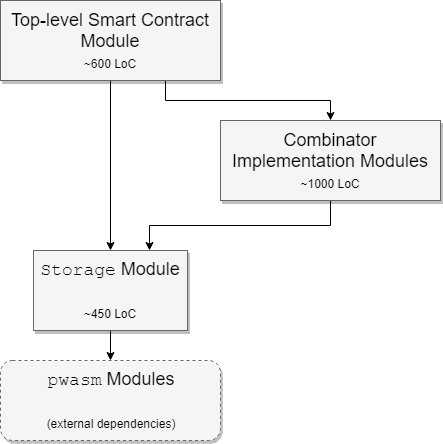
\includegraphics[width=0.5\textwidth]{smart-contract-block.png}
    \caption{A dependency graph of the modules used for the SmartFin smart contract, with their approximate \textit{Lines of Code} (not including tests). \texttt{pwasm} modules are external dependencies, described in section \ref{smart-contract-tech}. The combinator implementation modules are described in chapter \ref{combinators-main}.}
    \label{fig:smart-contract-block}
\end{figure}


\section{Requirements} \label{contract-requirements}

In order to ensure that the smart contract accurately and correctly represents SmartFin contracts, a set of requirements has been devised. These requirements form the motivation behind specific design and implementation choices made during the creation of the smart contract. \\

The SmartFin contracts that can be represented by the smart contract consist of an agreement between two parties (the \textit{holder} and \textit{counter-party}) with regards to payments between these parties. As such, the smart contract must hold the definitions of both the holder and counter-party, and allow the two parties to exchange funds through the contract. \\

The holder should have the ability to acquire the contract (just as they would be able to sign a traditional financial contract), and this should result in the evaluation of payments to be made between the two parties with respect to the acquisition time. \\

The smart contract should also be able to represent the behaviour/state of the combinators defined in section \ref{DSL-design}. The evaluation of the payments between the two parties should respect the semantics of these combinators. \\

Certain values in the SmartFin contract may be unknown until a later point (for example, observables in a \texttt{scale} combinator), and so the smart contract requires some way of obtaining these values. The holder may also be able to choose certain options on the SmartFin contract (for example, choosing a branch of an \texttt{or} combinator), and the smart contract should also facilitate this. \\

The evaluation of payments between the two parties may change over time. For example, the SmartFin contract \texttt{get truncate (01/01/2020 12:00) one} requires a payment to occur from the counter-party to the holder at noon on the 1st of January 2020. Before this time, no payments should occur. This means that the smart contract must be able to keep track of the state of the SmartFin contract's obligations over time. \\

All of these are specific requirements that are required for the smart contract to accurately represent any given SmartFin contract. These have been taken into consideration during the design and implementation of the smart contract, informing the final product.


\section{Design} \label{contract-design}

The overall design of the smart contract is fairly simple, albeit with several caveats. From a very high level, the smart contract consists of a class with an ABI, several state variables, and a tree of \texttt{ContractCombinator} objects. The behaviour of the SmartFin combinators is implemented by the \texttt{ContractCombinator} objects, the entire tree represent the SmartFin contract definition, and the rest of the smart contract effectively informs the way that it operates as a whole. See section \ref{combinators-design} for details on the representation of individual SmartFin combinators.


\subsection{High Level Design Challenges}

In an ideal world, the smart contract would track payments over time and exchange funds between the required parties immediately, as one might expect from a web-service or similar. Unfortunately, the smart contract runs on a blockchain, and as such there are several restrictions which affect its ability to operate as required. These inform the high-level design of the smart contract.

\subsubsection{Payment Evaluation}

It is not possible to schedule callbacks on a blockchain without relying on external tools, as this would jeopardise determinism, and it would require a miner to run the code at a specific time. As such, the smart contract is only able to perform execution when called into from a user. \\

Certain SmartFin contracts require payments to occur at specific times; for example, the contract \texttt{get truncate \textit{t} one} requires the counter-party to pay the holder 1 Wei at time \textit{t}. Unfortunately, smart contracts are unable to make payments at specific times, as this would require scheduled callbacks to be possible. \\

In order to represent time-respective payments, the implemented smart contract allows payments to be fulfilled retroactively. In essence, the smart contract does not perform payments at specific times, but instead keeps track of important times - typically combinators' acquisition times - and evaluates which payments should have occurred since that time after the fact. \\

To facilitate this, payments between the two parties are represented as a balance, changing when either party stakes/withdraws funds to/from the contract, or when payments are evaluated. In order to evaluate the payments which should have occurred by the current point in time, the smart contract has an \texttt{update} method which calculates the new balance between the holder and counter-party, resulting from any payments defined by the SmartFin contract definition between the last \texttt{update} call and the current block-time. For example, when the holder acquires the contract \texttt{get truncate \textit{t} one} before time \texttt{\textit{t}}, their balance does not change, and their balance does not change when \texttt{\textit{t}} passes either. Only once the contract is updated \textit{after} time \texttt{\textit{t}} does this balance change. This is depicted in figure \ref{fig:contract-update}. \\

\begin{figure}[h]
    \centering
    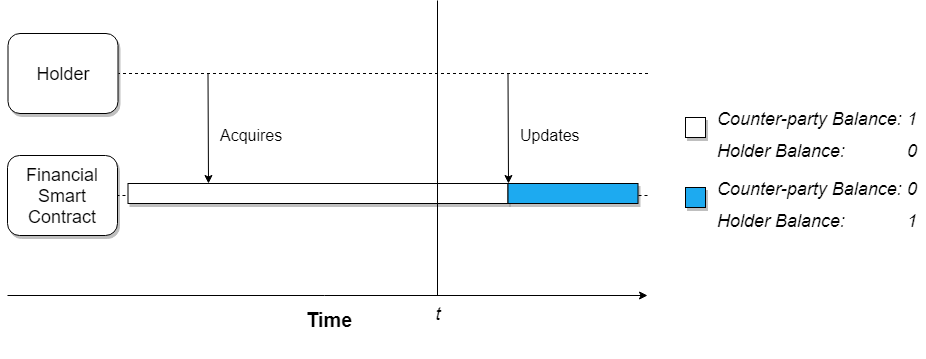
\includegraphics[width=\textwidth]{contract-update-diagram.png}
    \caption{A diagram depicting the balance of the holder and counter-party over time for the financial smart contract representing the SmartFin contract \texttt{get truncate \textit{t} one}.}
    \label{fig:contract-update}
\end{figure}

\subsubsection{Observable Evaluation}

Similar to the evaluation of payments, another factor in SmartFin contracts which changes over time is observables. These are objective, potentially time-varying quantities. An example of an observable which does not vary over time would be the number 5, whereas an example of an observable which does vary over time is the average temperature of London in Celsius. Both are objective, but one takes different values depending on what time you sample it. \\

Unfortunately, this poses a couple of problems for the smart contract. As mentioned earlier, smart contracts cannot schedule callbacks at specific times, and so finding the value of an observable at a specific time is not a simple task. There is also the issue that smart contracts are unable to access information which is not stored on the blockchain, which means that sampling observable values from websites or other off-chain sources is not possible. \\

These two restrictions effectively rule-out the possibility of the  smart contract obtaining the value of a time-varying observable without external interaction from the user. To work around this issue, when a SmartFin contract relies on an observable the author must define an \textit{arbiter} for its value. This arbiter is an address which can provide the observable's acquisition-time-value to the contract, effectively acting as a trusted source of information. \\

When an observable's value is unknown while the smart contract is being updated, the sub-contract relying on the observable will not be updated until the value is provided. After its provision, the sub-contract can be updated, thus allowing retroactive provision of observable values. For example, take the financial smart contract representing the SmartFin contract \texttt{scale \textit{x} <arbiter address> one}; when acquiring the contract before the observable's value is set, the balance does not change. Once the arbiter sets the value of the observable to 1, and then the financial smart contract is updated, the balance changes. This is depicted in figure \ref{fig:contract-scale-update}. \\

\begin{figure}[h]
    \centering
    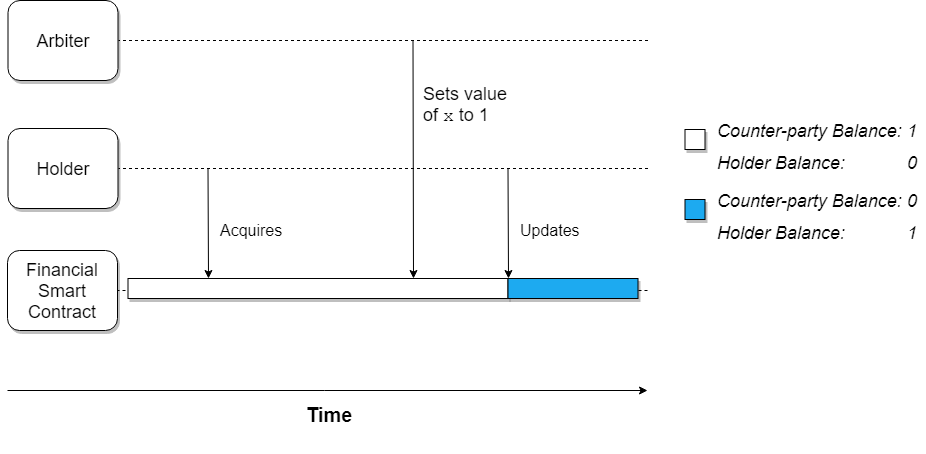
\includegraphics[width=\textwidth]{contract-scale-diagram.png}
    \caption{A diagram depicting the balance of the holder and counter-party over time for the financial smart contract representing the SmartFin contract \texttt{scale <observable name> <arbiter address> one}.}
    \label{fig:contract-scale-update}
\end{figure}

\subsubsection{Exchanging of Funds}

As you have hopefully noticed by now, smart contracts deal heavily with the exchanging of funds. Regular financial contracts are typically binding, requiring one party to pay the other party or risk legal action. Smart contracts are a little different; they have no way to ensure that one user will pay another user, but instead act as a separate entity which processes payments from both both parties. \\

A disadvantage of this is that the implemented smart contract is unable to force one party to pay the other party. It can maintain a balance between the two parties, indicating when one party \textit{should} pay the other, but it has no means to enforce this payment. In order to somewhat circumvent this issue, the smart contract allows users to stake Ether in the contract at any time (increasing their balance), and to withdraw Ether under certain conditions. In order to withdraw an amount of Ether: \\

\begin{itemize}
    \item The user must have enough Ether in their balance.
    \item The smart contract must have enough total balance.
    \item The user's balance must be larger than withdrawal gas fees (where gas fees apply). \\
\end{itemize}

By allowing the parties to stake Ether in the smart contract beforehand, the smart contract is able to make any required payments without immediate action from the paying party as long as it has enough funds. Incidentally, this is another reason that retroactive payments are appropriate, as there is no guarantee that the smart contract will actually have the funds to pay a party when a payment should occur. \\

Unfortunately, it is still impossible for the smart contract to solve the issue of binding a party to payment. As such, if one party decides not to pay, they can simply refuse to stake any Ether and thus the smart contract will have no funds to pay the other party. There were a few possible solutions (or at least mitigations) to this issue. \\

Restricting withdrawal from the smart contract until its conclusion would prevent parties from withdrawing before they have to make a payment. Unfortunately, it would also lower the value obtained through the contract, as funds locked in the contract's balance could instead be earning money through investment. Another potential solution could be to prevent contract acquisition until sufficient funds have been staked in the smart contract, but this has a similar issue that funds staked in a smart contract would be better served elsewhere. \\

The best solution to this issue is to use financial smart contracts alongside a legally-binding contract requiring a party to stake funds when required. For now, we assume that each party is bound to make payments to the smart contract in an honest way, as it seems that this is not something that can be solved in a satisfactory manner through the smart contract itself.


\subsection{Financial Smart Contract ABI} \label{smart-contract-ABI}

The smart contract has a set of functions which can be called by the web client, allowing it to interact with and monitor the contract. This ABI is informed by the requirements of the smart contract, and any caveats encountered due to its nature as a smart contract. The behaviour of many of these functions is determined by the composition of combinators used to write the SmartFin contract passed-in to the smart contract's constructor. The full financial smart contract ABI is listed in appendix \ref{appx:ABI}.


\subsubsection{Constructor}

The constructor of the smart contract is responsible for initialising the smart contract object, and as such it requires all information relevant to the initial state of the SmartFin contract. The constructor takes the following parameters: \\

\begin{itemize}
    \item The SmartFin contract definition.
    \item The address of the contract holder.
    \item Whether or not the contract should allocate gas fees upon withdrawal (as private blockchains do not always require gas fees).
\end{itemize}


\subsubsection{Pure Functions}

The smart contract defines several functions which return the value of state variables (i.e. \textit{getter} functions). This enables the web client to display the current state of the contract. As these are \textit{pure} functions, they do not cost any gas to call, and thus the web client may update its view of the smart contract as often as required at no cost. These functions consist of the following: \\

\begin{itemize}
    \item \texttt{get\_holder}: Returns the address of the contract's holder.
    \item \texttt{get\_counter\_party}: Returns the address of the contract's counter-party.
    \item \texttt{get\_contract\_definition}: Returns the SmartFin contract definition.
    \item \texttt{get\_balance}: Returns the balance of one of the parties (in Wei).
    \item \texttt{get\_concluded}: Returns whether or not the smart contract has concluded execution (i.e. no more updates are required).
    \item \texttt{get\_use\_gas}: Returns whether or not the smart contract allocates gas fees upon withdrawal.
    \item \texttt{get\_last\_updated}: Returns the block-time that the last call to the \texttt{update} function occurred at.
    \item \texttt{get\_acquisition\_times}: Returns a list of the acquisition times of the contract and its sub-contracts.
    \item \texttt{get\_or\_choices}: Returns a list of choices which have been made for \texttt{or} combinators.
    \item \texttt{get\_obs\_entries}: Returns a set of observables, including their names, values, and arbiter addresses.
\end{itemize}

\subsubsection{Setting Values}

The smart contract has several values which rely on user input to evaluate. One such combinator is the \texttt{or} combinator, which allows the holder to acquire either of its two sub-contracts at the time of acquisition. The holder is able to call the function \texttt{set\_or\_choice} at any time, to inform the smart contract of which sub-contract the holder should acquire for a given \texttt{or} combinator. An \texttt{or} choice cannot be changed after it has been made, to prevent inconsistency across multiple updates. \\

Another combinator which requires user input is the \texttt{scale} combinator. For each \texttt{scale} combinator's observable, if said observable is not a constant then it will require an arbiter to provide its value. The arbiter can call the \texttt{set\_obs\_value} function to set the value of an observable at any time, once per observable.

\subsubsection{Acquisition}

The holder must have the ability to acquire the smart contract, just as a prospective holder would be able to acquire a traditional financial contract by signing it. As such, the smart contract's ABI contains an \texttt{acquire} method, callable by the holder. This method updates the contract state to store the time of acquisition. \\

Besides the top-level contract, \texttt{anytime} combinators can also be acquired at certain times during the smart contract's lifetime. As such, there is also an \texttt{acquire\_anytime\_sub\_contract} method; if the acquisition is valid (i.e. the \texttt{anytime} combinator's parent is acquired, and the combinator is not expired), then the smart contract will update its state to reflect that the sub-contract has been acquired.

\subsubsection{Update}

Due to the nature of the blockchain, the smart contract cannot keep itself up-to-date without external action. The \texttt{update} function causes the smart contract to evaluate the difference in balance between the current \texttt{update} call and the last \texttt{update} call, retroactively evaluating payments. The \texttt{update} function can be called from any address, as the update operation is handled entirely by the smart contract with no external inputs.

\subsubsection{Payment and Withdrawal}

The smart contract allows either party to stake Ether, to facilitate payments between them. The \texttt{stake} method is a \textit{payable} function (i.e. it can receive Ether), which increases the balance of the party that called it by the amount of Ether received. \\

The smart contract also allows either party to withdraw Ether, assuming the balances allow it. To do this, the \texttt{withdraw} method takes an amount and sends the requested amount of Ether to the calling party, reducing their balance by the withdrawn amount. Gas fees (when enabled) are taken out of the party's balance on top of the withdrawal, or out of the withdrawal amount if the balance hits 0. Besides the two involved parties, no addresses can stake or withdraw Ether - it would be unclear who to allocate staked Ether to, and only the respective party should be able to withdraw from their balance.


\section{Implementation}

\subsection{Technologies} \label{smart-contract-tech}

In order to implement the smart contract, there were several choices to make with regards to which technologies would be employed. As discussed in section \ref{DSL-implementation-technologies}, there are many possible tools with which to implement a smart contract. \\

The final method that was decided upon for implementing the smart contract was the use of Rust\cite{rust} with \textit{pwasm} modules/tools provided by Parity Technologies\cite{parity-technologies} for compilation to WebAssembly. The final WebAssembly contract is compatible with private blockchains run from Parity's own Ethereum client, as well as with the Kovan test network and other wasm-compatible Ethereum clients\cite{pwasm-tut-node}. \\

The pwasm modules provide various tools for developing smart contracts in Rust, as discussed in section\ref{dev-tools}. The main tools which were made use of in the smart contract implementation were: \\

\begin{itemize}
    \item \texttt{pwasm-std}: A module re-implementing useful pwasm-compatible functionality from the Rust standard library (which is not compatible with these pwasm modules).
    \item \texttt{pwasm-ethereum}: A module providing access to information and functionality from the blockchain, including the current block-time, the address of the caller, writing to or reading from smart contract storage, and more.
    \item \texttt{pwasm-abi} and \texttt{pwasm-abi-derive}: Modules which enable the conversion of a Rust trait into a smart contract ABI definition.
    \item \texttt{pwasm-test}: A unit testing framework for smart contracts written in Rust. \\
\end{itemize}

Unfortunately, due to the pwasm modules' incompatibility with the Rust standard library, it was impossible to use most external modules for the Rust smart contract. The smart contract implementation was possible without requiring any more external modules, but certain problems like serialization of structs could be solved much more easily using external libraries if it were possible. \\

In order to build the Rust smart contract, \textit{Cargo}\cite{cargo} (the Rust package manager) was used. Parity also provides a build tool for building wasm contracts with Cargo, \textit{wasm-build}\cite{pwasm-build-tools}. \textit{Web3.js}\cite{web3-intro} was also used to deploy smart contracts to the blockchain, and interact with them (for testing purposes). This was managed with \textit{yarn}\cite{yarn}, a package manager for JavaScript.


\subsection{Smart Contracts in Rust}

Rust smart contracts implemented using the pwasm modules must be defined in a particular manner. Firstly, the Rust program must have a few things implemented in the main module of the application (typically written in \texttt{lib.rs} for a Rust program), including a smart contract ABI, a smart contract struct, and a \texttt{call} and \texttt{deploy} function. \\

The smart contract's ABI is defined through a trait (a set of several methods) with annotations. Pure methods (i.e. those that do not alter smart contract state) are denoted by the \texttt{constant} annotation, and payable methods (i.e. those that can receive Ether) have the \texttt{payable} annotation. There must also be a \texttt{constructor} method implemented, which initialises the smart contract struct/state on deployment. This trait is then used to generate the smart contract ABI, as well as to generate an \textit{endpoint} which delegates method calls to the smart contract struct. Only certain types are able to be sent/received via a pwasm smart contract's ABI, including integer types, vectors, addresses, booleans, and a few more binary data types. \\

A smart contract struct must also be implemented. This is a data type which must implement the ABI trait. Every time the smart contract is called into, a new instance of the smart contract struct is constructed. This means that member variables on the struct will be reset every time that the smart contract is called into. In order to store persistent state across smart contract calls, the smart contract storage must be manually written to/read from (using methods provided by \texttt{pwasm-ethereum}). \\

Alongside the ABI and smart contract struct, public static \texttt{call} and \texttt{deploy} functions must be implemented. The \texttt{call} function will initialise the smart contract struct, and an \textit{endpoint} which delegates method calls based on the ABI, and handles smart contract calls by providing the call inputs (method name, parameters, etc.) to the endpoint. The \texttt{deploy} function is similar, but is called when the smart contract is first deployed to forward the inputs for the constructor call to an initialised endpoint.


\subsection{ABI Methods}

\subsubsection{Constructor}

The constructor is called when the smart contract is initially deployed, and is responsible for setting up the initial state. Firstly, the validity of the constructor arguments is checked, throwing an error if any invalid arguments are passed; throwing an error will cause smart contract methods to cease execution and roll-back state changes. After checking the arguments, the constructor writes several values to storage, including the holder and counter-party addresses, the holder and counter-party balances, whether or not the contract uses gas, the last-updated time, and the contract definition. \\

The contract definition is passed to the constructor as the type \texttt{Vec<i64>}, i.e. a vector of signed 64-bit integers. This is necessary as Rust smart contracts written with pwasm modules cannot send/receive strings over the ABI, and thus the contract definition must be provided in a serialized form. The serialized form of SmartFin simply involves representing the SmartFin contract as an array of integers. Each combinator is represented by an integer (0 to 9), times are represented as UNIX Epoch times, integer values are unchanged, names are represented by arrays of character codes, and addresses are represented by an array of four integers. The contract definition is deserialized recursively into a set of \texttt{ContractCombinator} objects, representing the SmartFin combinators. For more information on how the combinators are represented in the Rust smart contract, see chapter \ref{combinators-main}.


\subsubsection{Pure Methods} \label{ABI-pure}

The pure ABI methods (i.e. getters) are generally quite straightforward; \texttt{get\_holder}, \texttt{get\-\_counter\_party}, \texttt{get\_contract\_definition}, \texttt{get\_balance}, \texttt{get\_use\_gas}, \texttt{get\_last\_updated}, and \texttt{get\_acquisition\_times} all read the required data from storage and return it in a trivial manner. \\

\texttt{get\_concluded} returns \texttt{true} if the contract will no longer change state over time, i.e. all responsibilities are fulfilled. This is true if the contract has been acquired and the combinators have been fully updated to their final state, or if the contract has expired before acquisition. \\

\texttt{get\_or\_choices} reads the set of choices for \texttt{or} combinators from storage, and then serializes this into a vector of bytes. \texttt{1} represents the first sub-contract, \texttt{0} the second, and \texttt{2} means that no choice has been made yet. \\

\texttt{get\_obs\_entries} constructs and returns the set of observable entries for the contract from storage. This consists of a vector of observables, with their arbiter address, value, and name (all serialized as several signed 64-bit integers).


\subsubsection{Sub-contract Acquisition and Setters}

The functions setting \texttt{or} combinator choices, observable values, and acquiring \texttt{anytime} sub-cont\-racts are also quite straightforward. The \texttt{or} choices, observable values, and \texttt{anytime} acquisition times are all stored as vectors in the smart contract storage. In order to update any of these values, the relevant element in the vector is written to directly through a storage object, described in section \ref{storage}. Acquiring an \texttt{anytime} combinator's sub-contract will also update the contract, with a call to \texttt{update}.


\subsubsection{Acquire}

The \texttt{acquire} method first reads and deserializes a combinator object from storage, which implements a combinator contract's behaviour. If the caller is the holder and the combinator hasn't been acquired already, the method calls an \texttt{acquire} method on the contract combinators, passing down a reference to the storage object. For more information on the combinator objects' \texttt{acquire} methods, see section \ref{combinator-implementation}. The combinator object is then serialized and re-written into storage.


\subsubsection{Update}

The \texttt{update} method first checks if the contract has concluded. If so, then updating the contract will have no effect no matter what happens, so the contract throws an error. After this, the combinator object is read from storage and deserialized, as in the \texttt{acquire} method. The storage object is passed to the \texttt{update} method on the combinator object, which is also described in section \ref{combinator-implementation}. The combinators are then serialized and written back to storage. \\

After updating the combinators, the new balances of the holder and counter-party are written to storage. These are calculated using a \texttt{safe\_add} method, which checks for integer overflow. Rust should throw an error automatically if it occurs, but extra precaution is taken due to the severity of overflow errors with balances in smart contracts.


\subsubsection{Stake}

The \texttt{stake} method is a \texttt{payable} function, to which Ether is paid upon calling. The \texttt{pwasm-ethereum} function to obtain the value of a transaction returns a \texttt{U256}, i.e. an unsigned 256-bit integer. Balances are stored in the smart contract storage as signed 64-bit integers, as they are easier to work with being Rust primitive types. Because of this, the \texttt{stake} method must first check that the value provided can be converted into a signed 64-bit integer, or an error is thrown. \\

After checking this, the method checks whether the caller is the holder or the counter-party - an error is thrown otherwise. The method then safely adds the value of the method call transaction to the balance of the relevant party, and writes the new balance to storage.


\subsubsection{Withdraw}

The \texttt{withdraw} method allows a user to withdraw funds from the contract by initiating a transfer of Ether from the smart contract to the caller. First, the method checks which address to withdraw Ether from. If the caller is not one of the holder or the counter-party, then an error is thrown. \\

The method calculates how much Ether to send by comparing the amount requested to the balance of the relevant party, the total contract funds, and the gas cost. If the contract allocates gas fees upon withdrawals, then 2300 Wei in gas fees is added to the withdrawal amount. If either of the total funds of the contract or the party's balance are smaller than the gas cost, then an error is thrown. The withdrawal amount (including gas fees) is clamped to the minimum of the party's balance and the total funds. If the final amount is 0 or less, then an error is thrown. \\

After the viable withdrawal amount is calculated, the relevant balance is updated, and then the method creates a transaction from the smart contract to the caller address. If the transaction fails then the relevant balance is rolled back to its original amount, and an error is thrown.


\subsection{Storage} \label{storage}

Besides the ABI methods and combinator behaviours, the other main functionality that the smart contract implemented was storage. State - such as the holder address, acquisition times, or the combinator objects - must be stored in smart contract storage in order to remain persistently across multiple smart contract method calls. In order to do this, the \texttt{Storage} module was implemented to handle the storage of various data types.


\subsubsection{Memory Layout of Smart Contract Storage}

Smart contract storage is addressed using 256-bit integers (of the type \texttt{H256}), and each slot in storage can store 256 bytes of information in the form of an array of 32 unsigned 8-bit integers. In order to separate storage into different spaces, the most-significant byte of each memory address is treated as a "namespace" byte by the smart contract. The hexadecimal addresses \texttt{0x0000...00} to \texttt{0x00FF...FF} span the first memory namespace, \texttt{0x0100...00} to \texttt{0x01FF...FF} span the second memory namespace, etc. As such, if a function is writing to storage sequentially and reaches the end of a namespace, by incrementing the most-significant byte, then an error must be thrown.


\subsubsection{Storage Module Design}

The \texttt{Storage} module contains definitions for a \texttt{Storage} struct and several traits which include methods to read from/write to smart contract storage. The reason that a struct is used instead of static methods is that data read from/written to smart contract storage is cached in the Storage object, and so only one read to smart contract storage must occur for each object being read per ABI method call. The cache is destroyed between ABI method calls as the smart contract struct is destroyed after the ABI call finishes and the smart contract is exited. Cached reads/writes are stored in a vector of \texttt{Entry} struct instances, which contain the storage address and a value. \\

There are also three generic traits which are used for storage; the \texttt{StoresFixed<T>} trait indicates that the implementing struct can store a value of the type \texttt{T} in memory, and that the size of any values of this type is constant. The size restriction is helpful as it ensures that values can be stored sequentially in smart contract storage without changing in size and overwriting each other, or leaving empty space between elements. The trait defines methods for reading/writing a value, and a static \texttt{size} method. \\

The second generic trait used for storage is \texttt{StoresFixedVec<T>}, which indicates that the implementing struct can store an object of the type \texttt{Vec<T>} in memory, where elements of type \texttt{T} have a known fixed size. This trait allows reading/writing the whole vector to storage with linear time complexity, as well as getting the length, reading/writing individual elements, and pushing elements to the end of the array with constant time complexity. \\

The third trait used for storage is \texttt{StoresVariable<T>}, which indicates that the indicating struct can store an object of the type \texttt{T} in memory, but its size is unknown and/or variable. This trait allows writing or reading of whole objects of type \texttt{T} with linear time complexity. \\

All write and read methods return a key along with any other value. This key represents the last storage address used in the method. For example, if a vector is stored at address 2 and takes up 6 slots, the read/write methods will return address 7. This enables sequential writing of values in memory, especially useful when those values have variable size.


\subsubsection{Storage Method Implementation}

Besides several implementations of the traits mentioned above, the \texttt{Storage} struct also has method implementations for several of its own helper methods, for converting values between types. The \texttt{Storage} struct also has a constructor which will initialise the storage cached vector to empty. \\

Only one type can be read from/written to smart contract storage using the \texttt{pwasm-ethereum} \texttt{read}/\texttt{write} functions, an array of 32 unsigned 8-bit integers (i.e. \texttt{[u8; 32]}). Several methods on the \texttt{Storage} struct implement conversion of other types to/from this type. The \texttt{from\_address} method converts an address into an \texttt{H256} data type using the \texttt{H256::from} function, which can be converted directly into a \texttt{[u8; 32]} object. The method \texttt{to\_address} converts similarly in the opposite direction. \\

The \texttt{from\_bool} method converts a boolean value into \texttt{[u8; 32]}. In the case of \texttt{false}, the function returns a \texttt{[u8; 32]} array with all elements set to 0, otherwise an element is set to 1. The \texttt{to\_bool} method can thus return whether or not the given \texttt{[u8; 32]} is not equal to \texttt{H256::zero()}. \\

The last pair of conversion functions that the \texttt{Storage} struct implements is \texttt{to\_i64} and \texttt{from\_i64}. As the \texttt{pwasm-std} module implements functions \texttt{read\_u64} and \texttt{write\_u64}, which convert an unsigned 64-bit integer (i.e. \texttt{u64}) to/from \texttt{[u8; 32]}, the \texttt{i64} conversion methods use this method and convert between \texttt{i64} and \texttt{u64}. \\

To convert from a \texttt{u64} to an \texttt{i64}, first the value of the \texttt{u64} is checked. If the \texttt{u64} value is less than $2^{63}$, then it can be directly converted to an \texttt{i64}. This is because binary representation of an integer in the range of $0$ to $2^{63} - 1$ is equivalent for both types. For an n-bit unsigned integer, the value can be calculated as $2^0 \cdot b_0 + 2^1 \cdot b_1... + 2^{n-1} \cdot b_{n-1} + 2^n \cdot b_n$, where $b_i$ is the value of the \texttt{i}'th least significant bit. For an n-bit two's complement integer, the equivalent expression would be $2^0 \cdot b_0 + 2^1 \cdot b_1... + 2^{n-1} \cdot b_{n-1} - 2^n \cdot b_n$. As such, as long as the most-significant bit is 0, then the decimal value of an \texttt{i64} and a \texttt{u64} with the same binary representation is equal. If the \texttt{u64}'s most significant bit is 1, then we can convert to two's complement by subtracting $2^{64}$. This must be done in a slightly roundabout manner in Rust, by subtracting $2^{63}$ to convert the \texttt{u64} into the range of an \texttt{i64}, and then subtracting $2^{62}$ twice (as $2^{63}$ cannot be represented as an \texttt{i64}). The reverse conversion from \texttt{i64} to \texttt{u64} is similar, requiring $2^{64}$ to be added rather than subtracted.


\subsubsection{Static Storage Module Functions}

The \texttt{Storage} module also provides several static functions. Functions for converting between an \texttt{Address} and an array of four \texttt{i64}s are provided. To convert from an \texttt{Address} to four \texttt{i64} values, \texttt{address\_to\_i64} converts the address to a storable \texttt{[u8; 32]} array using \texttt{Storage::from\_address}. This array is split into four separate 32-byte storable values, where the first 8 bytes of each is a quarter of the storable value, and the rest are 0. These can be converted to an \texttt{i64} using \texttt{Storage::from\_i64}. The function \texttt{i64\_to\_address} works similarly in the opposite direction. \\

The \texttt{Storage} module also provides a private function \texttt{add\_to\_key}. This function takes a storage key (as an \texttt{H256}) and an unsigned 64-bit integer value, and increments the address by the value. This is done by repeatedly incrementing the least-significant bit of the address, and decrementing the value, until the value hits zero. If the least-significant bit overflows, then it is set to 0 and the next least-significant bit is incremented. This is repeated if the next least-significant bit is incremented. If the second most-significant byte overflows, than an error is thrown as this would violate the separation of memory namespaces mentioned in the \textit{Memory Layout of Smart Contract Storage} segment of this section.


\subsubsection{\texttt{StoresFixed} Implementation for \texttt{[u8; 32]}}

For the \texttt{write} method implementation, the storable array is first written into the smart contract storage using \texttt{pwasm-ethereum}'s \texttt{write} method. After this, the \texttt{Storage} struct's cache is checked for the presence of the given key. If the key is present, the value is updated to the new value provided, otherwise it is added to the table. For the \texttt{read} implementation, the cache is checked for the presence of the given key. If this hits, then the corresponding value is returned, otherwise it is read from smart contract storage and written into the cache before being returned. The storage address returned from both of these methods, representing the last-used address in writing the given object to storage, is the same as the key passed in - this is because a \texttt{[u8; 32]} value can be stored in one storage slot. \\

\subsubsection{\texttt{StoresFixed} Implementation for Primitive Types and Address}

As mentioned earlier, the \texttt{Storage} struct implements several conversion methods between primitive types (\texttt{u32}, \texttt{i64}, \texttt{bool}) or \texttt{Address} values and storable values (\texttt{[u8;32]}). Leveraging this, the \texttt{StoresFixed} implementations for these types simply convert the values into a \texttt{[u8; 32]} value and call into the \texttt{StoresFixed<[u8; 32]>} implementations.


\subsubsection{\texttt{StoresFixed} Implementation for \texttt{Option<T>}}

In order to store values of type \texttt{Option<T>} (which take the value \texttt{None} or \texttt{Some(v: T)}), we must be able to store values of type \texttt{T} and a value to indicate whether or not the object has a concrete value. The \texttt{write} method for \texttt{Option<T>} will pattern match the given value, and write a boolean \texttt{true} or \texttt{false} depending on whether a concrete value exists. If one exists, it is written to the next slot in storage; if not, nothing is written to the next slot in storage. Either way, the last-used key returned is the passed-in key plus the size of \texttt{T} in storage, in order to reserve a second slot in storage regardless of whether a value was written (or else the storage size of \texttt{Option<T>} would not be fixed). The \texttt{read} method simply checks if a value is stored or not, then reads and returns \texttt{Some(value)} or \texttt{None}.


\subsubsection{\texttt{StoresFixedVec} Implementation}

Vectors are stored in smart contract storage sequentially, with the first storage slot containing the number of elements in the vector, and the following slots containing values written using the \texttt{StoresFixed<T>} implementation. Vectors are always written in their own memory namespace - i.e. their most-significant byte is unique - to prevent a change in size from overwriting adjacent values in storage. \\

The \texttt{write\_vec} implementation gets the length of the given vector and writes that to the first storage slot. After this, the vector is processed to write each element into storage sequentially. The last-used key is kept track of throughout this process, and returned after the whole vector is stored. The \texttt{read\_vec} implementation is similar, first reading the vector length and then reading the elements sequentially from storage into a new vector, returning the last-used key. The \texttt{length} method simply reads the length from the first storage slot of the vector, and \texttt{set}/\texttt{get}/\texttt{push} which deal with individual vector elements will find the address of the required index by calculating the starting address plus the size of storing values of type \texttt{T} multiplied by the index.


\subsubsection{\texttt{StoresFixed} Implementation for Tuples}

\texttt{StoresFixed} is implemented for tuples with two and three elements, where an implementation of \texttt{StoresFixed} exists for all element types. This allows the smart contract to store small generic sets of data without implementing a specific struct, like an observable's arbiter, name, and value. Tuples are stored sequentially in memory, which is trivial using the \texttt{write}/\texttt{read} implementations of the tuple element types.


\subsubsection{\texttt{StoresVariable} Implementation for Vectors and Observable Names}

When the smart contract is constructed, a set of serialized observable names is generated from the given combinator contract. These are represented by a vector of integers per observable name; to store these names, a vector of vectors must be stored. As a vector of integers can grow and shrink, a \texttt{StoresFixedVec<Vec<T>{}>} implementation cannot be used. As such, \texttt{StoresVariable} exists to allow writing/reading variable-sized objects to and from storage in their entirety. \texttt{StoresVariable} is implemented for \texttt{Vec<T>} where \texttt{StoresVariable<T>} is implemented, and for \texttt{ObsName} - a struct containing the serialized observable name vector. The implementations are similar to the \texttt{StoresFixedVec<T>{}>} implementation, without the element-wise methods.


\section{Evaluation} \label{DSL-impl-evaluation}

In order to evaluate the design of the smart contract (minus combinator implementations), there are a couple of methods that can be employed. Qualitative analysis of the design of the smart contract's ABI can evaluate how well the smart contract fulfils the requirements laid out in section \ref{contract-requirements}. Qualitative analysis of the \texttt{Storage} module can also be employed to evaluate its design. Automated tests have also been used to ensure that the smart contract operates correctly, as described in section \ref{contract-design}, and that the \texttt{Storage} module operates as expected.

\subsection{Design of the Smart Contract's ABI}

To evaluate the smart contract's ABI, it can be compared to the requirements laid out in section \ref{contract-requirements}. The first requirement described the requirement that a financial smart contract should represent an agreement between a \textit{holder} and a \textit{counter-party}, and should allow the two parties to exchange funds. This is implemented in the contract by storing the holder and counter-party's addresses, and the staking and withdrawal of funds from the smart contract allows an indirect exchange of funds between the two parties.

Unfortunately, the smart contract does not facilitate direct payments between the two parties, but this would be impossible as a smart contract cannot initiate a transaction with another user's funds. Another issue with this implementation is that payments do not occur in real time, but instead retroactively through the \texttt{withdraw} method. Due to the lack of scheduled callbacks, and the requirement that funds are staked before being sent by a transaction, this would also not be possible. Retroactive payments are the next best option, and are not too dissimilar to the way that some financial contracts would handle transactions, e.g. via an escrow mechanism. \\

The second requirement was that the holder should be able to \textit{acquire} the contract, which should result in the evaluation of payments between the holder and the counter-party, with respect to acquisition time. This is implemented through the \texttt{acquire} method on the smart contract, allowing the holder to acquire it at any point in time, and evaluating payments required between the two parties - represented by a balance for each party. Assuming that the evaluation of these payments is correct (discussed in section \ref{contract-testing}), then this requirement is aptly fulfilled. \\

The third requirement, requiring the evaluation of payments to respect the given financial combinator contract's expected behaviour, is handled by the implementations of the combinators. This is detailed in section \ref{combinators-main}. \\

The fourth requirement requires the setting of observable values and \texttt{or} combinator branch choices to be possible. The setting of observable values is implemented through the \texttt{set\_obs\_value} method on the smart contract's ABI, which allows pre-defined arbiters to provide the values of observables. Ideally, the observables' values could be obtained automatically by the smart contract, but due to the lack of scheduled callbacks or off-chain interaction this is not possible. The implemented solution is the next best option.

The choosing of \texttt{or} combinator sub-contracts is implemented via the \texttt{set\_or\_choice} method on the ABI, allowing the holder to choose which sub-contract to acquire when the given \texttt{or} combinator is acquired. This works similarly to how a real financial contract works, where the holder must choose the sub-contract by making a choice manually, and so the requirement is fully met. \\

The final requirement described earlier is for the smart contract to keep track of the evaluation of payments over time. This is handled by keeping track of the balance of the holder and counter-party, and by updating it retroactively through calls to the \texttt{update} method in the smart contract's ABI. This method evaluates the difference in balance due to payments occurring since the last \texttt{update} call, thus keeping track of payments over time. Assuming that evaluation of payments is correct, as evaluated in section \ref{contract-testing}, then this method of keeping track of payments over time is sufficient to fulfil this requirement. \\

Based on these requirements - while there are some issues due to the lack of scheduled callbacks, off-chain interactions, and so-on - the final implementation is still sufficient to represent a traditional financial contract as a smart contract with similar behaviour. \\

Besides these requirements, there is one issue which plagues the smart contract's ABI: serialization. Most methods involve some level of serialization, with serialized arguments or return types. The reason that this is an issue is that it causes the smart contract to be very difficult to interact with from a command-line. Unfortunately, this issue is somewhat unavoidable due to the inability to send strings over a smart contract ABI implemented with \texttt{pwasm-abi}; implementing the smart contract in another language, like Solidity, may have avoided this however. The issue is also somewhat assuaged by the existence of the web client, through which most interaction with financial smart contracts should occur. For anyone aiming to write a financial contract, it would likely preferable to use a web client with lower requirements of technical skill compared to a command-line interface anyway. As such, the problem is not a deal-breaker.


\subsection{The \texttt{Storage} Module}

Another major component of the smart contract implementation is the \texttt{Storage} module. While there are no specific requirements of the \texttt{Storage} module with regards to the project as a whole, it can still be evaluated in regards to its design and performance. \\

The use of generic traits to handle the storage ABI results in a simple, easy to use \texttt{Storage} struct where most implemented types can be written/read using only one method. This trait design is also reusable, and is not specific to the smart contract storage model; while this is not essential for this project, it is an indicator that the design of the traits handles encapsulation well. \\

All of the storage trait implementations handle writing and reading in linear time at worst, and constant time at best. The element-wise lookup/update functionality for most vectors is very useful, resulting in most operations which write to storage in the contract taking constant time. In an Ethereum smart contract, extra complexity can result in the user spending more in gas fees to call a function - the more operations a function call carries out, the higher the gas cost in Ether. While this project may not be ideal for use on public blockchains, and may be more useful in the context of private blockchains within/between financial organisations where gas is less of an issue, the lower usage of resources is a benefit no matter what. While variable-sized values must be read/written in their entirety, taking linear time, this is not a huge issue - the only variable-sized value stored in the smart contract is the vector of observable names. This is only written to at the beginning of the contract, and always read and returned in its entirety when \texttt{get\_obs\_entries} is called - the latter usage is part of a pure function, however, and thus costs no gas anyway. As such, the impact is minimal. \\

One potential area for improvement in the \texttt{Storage} module is the amount of storage used. For example, storing an \texttt{Option<i64>} requires storing a \texttt{bool} in one storage slot, followed by an \texttt{i64} in the following storage slot. In total, this takes 65 bits. A smart contract storage slot stores up to 256 bits of information, so this information could be stored in 1 storage slot. Because of the generic trait system, it is difficult to optimise the amount of space objects with sub-values take. Furthermore, it would require much more specific implementation based on the type of the value being stored, which would quickly become complex and unwieldy, and require much more effort to implement. As such, the current implementation is preferred, but optimisations - like reducing storage sparsity by serializing combinators directly to byte arrays instead of integers - could definitely be implemented. \\

Another interesting aspect of the \texttt{Storage} struct is that it implements a key/value cache. The aim of this is to reduce the performance hit of reads when the same address is read from multiple times in one financial contract ABI call. One issue with this is that in general, no ABI call will write to/read from the same address more than once; acquiring and updating the contract only updates each combinator once, and other function calls are not iterative or recursive besides the constructor. This could potentially mean that the performance hit of maintaining the cache does not have enough of an upside to make it worthwhile. This is difficult to evaluate concretely, but it is possible that the implementation of a cache is not improving efficiency in this context.


\subsection{Automated Testing} \label{contract-testing}

In order to ensure that the behaviour of the smart contract is correct, the most obvious tool to use would be automated testing. A suite of unit tests was written for the main smart contract module, as well as a unit test suite for the \texttt{Storage} module, and a set of integration tests for the smart contract, \texttt{Storage}, and combinator modules. \\

One important note is that for any of the smart contract tests written in Rust, the top-level smart contract struct was not deleted between function calls (which would occur in real-world operation on a blockchain). This means that all reads from storage would hit in the \texttt{Storage} struct's cache, and so reading from and writing to actual smart contract storage are not tested in Rust. The conversion between types is still tested, however, and the writing to/reading from storage relies on the correctness of the \texttt{pwasm-ethereum} storage methods - as such, this is an acceptable compromise. There are also JavaScript integration tests for the smart contract, which \textit{would} have the smart contract struct deleted between function calls - thus requiring the use of smart contract storage. Besides this, there should be no meaningful differences between the Rust test environment and real-world operation.


\subsubsection{Smart Contract Unit Tests}

The general testing philosophy for the smart contract ABI functions is fairly simple; for every function in the ABI, the expected functionality should be fully covered by tests, and cases where errors are thrown should all be tested. The \texttt{pwasm-test} module enables unit testing of the smart contract with mocking of calls to \texttt{pwasm-ethereum} (e.g. to find the sender of the contract call transaction). This was used with Rust's normal testing framework for all unit tests. There are 37 unit tests made up of ~650 LoC (Lines of Code) for the top-level smart contract module. \\

To ensure that the holder, counter-party, and contract definition are correctly stored after the constructor, tests on the top-level getter functions for these values have been implemented. \\

The \texttt{update} method is tested to ensure that it does nothing before acquisition, calls into the combinators correctly after acquisition, and sets the last-updated time. The calculation of the balance of the two parties is also checked in one test each. Assuming that the combinators operate correctly, this covers its functionality. The \texttt{acquire} method is tested alongside the \texttt{update} and \texttt{get\_acquisition\_times} methods, as it does not change state in an externally-visible way on its own. \\

The setters and getters for observables and \texttt{or} combinator choices, and \texttt{anytime} combinators' acquisition method are all tested by calling the setters/acquire method, and checking the resulting observable values, \texttt{or} choices, and \texttt{anytime} acquisition times respectively. \\

The helper function for the \texttt{withdraw} method is checked to ensure that the correct withdrawal amount is calculated under all special cases, i.e. with sufficient funds/balance and with/without gas fees, with insufficient funds and with/without gas fees, with insufficient balance and with/without gas fees, and with balance/funds below the gas price when gas fees are not used. \\

Besides these functionality tests, errors in the main smart contract module are tested under conditions where the errors should be thrown, and by expecting the error. If no error is thrown, or the error thrown does not match the expected error string, the tests fail. All potential errors in the smart contract are tested this way.


\subsubsection{\texttt{Storage} Unit Tests}

In order to ensure that the smart contract operates correctly, it must be the case that the writing and reading of data to and from storage is correct, i.e. that after writing a value to a storage address, reading from the same address returns an equivalent value. In order to test this, each storage trait implementation is tested, as well as the public functions to convert between addresses and signed 64-bit integers. There are 15 unit tests made up of ~150 LoC for the \texttt{Storage} module. \\

For each \texttt{StoresFixed<T>}, \texttt{StoresFixedVec<T>}, or \texttt{StoresVariable<T>} implementation, a test function exists which writes several values of the type T to storage, and then reads them back. The original values and the values read from storage must be equal, or else the test fails. For \texttt{StoresFixed<T>}, the \texttt{size} functions are also checked.


\subsubsection{Integration Tests}

There are several integration tests written in Rust, designed to ensure that the behaviour of the contract is correct throughout multiple method calls. The majority of these tests involve supplying a contract definition, supplying any required inputs, and acquiring/updating the contract - the final balances are then checked to ensure that contract evaluation acts correctly as a whole. In total, there are 25 Rust integration tests made up of ~400 LoC, and 25 JavaScript integration tests made up of ~350 LoC. \\

There is at least one Rust integration test for each combinator, involving contracts written using the combinator in question. Evaluation of the behaviour of the combinators is left for section \ref{combinators-eval}, these tests instead focus on checking of the entire flow of the smart contract's execution. For an example, the test for the smart contract with the combinator contract \texttt{one} supplies the contract definition, acquires the contract, and checks the balance. This tests that the flow through the smart contract over time is correct. \\

Several of these integration tests require the use of extra smart contract ABI methods. The \texttt{set\_or\_choice} method is tested for left and right or choices, \texttt{truncate} is tested with the acquisition time before and after the horizon, \texttt{set\_obs\_value} is tested with a contract with an observable, and \texttt{acquire\_anytime\_sub\_contract} is tested with a contract with an \texttt{anytime} combinator. \texttt{get\_concluded} is also tested, both by expiration and by updating. \\

Besides the Rust integration tests, there is also a large suite of integration tests written in JavaScript. These tests deploy the smart contract to a private Ethereum blockchain node (running in the Parity client), and make calls to the contract using the Web3.js library. While these tests are stored with the tests for the web client (for ease of running tests/building), they only test the smart contract functionality. \\

These JavaScript tests are written similarly to the Rust integration tests; for each type of combinator, there are tests of its expected behaviour. There are also tests which ensure that payment in Ethereum operates correctly, ensuring that the smart contract obtains staked Ether, and that the relevant parties obtain Ether when withdrawing it.

\subsection{Conclusion}

Overall, the smart contract's ABI fulfils the requirements laid out in section \ref{contract-requirements} to the best level that can be achieved given the limitations of Ethereum smart contracts, or at least close to it. The \texttt{Storage} module is fairly efficient and well designed, but the cache implementation may not be as beneficial as one would hope. Thorough automated testing helps to support the correctness of these modules, all of which pass.


\section{Remarks}

In this chapter, the design and implementation of the smart contract which can represent any SmartFin contract has been described in detail. The final result is a smart contract which implements all of the required functionality of a SmartFin contract about as accurately as possible - including an ABI for interacting with the smart contract, and persistent storage of the smart contract state - with few issues. \\

While this section covers most of the smart contract implementation, the implementation of the SmartFin combinators' behaviour has not yet been described; in the following chapter, the smart contract representation of these combinators is laid out in detail.


\chapter{Designing and Implementing SmartFin Combinators} \label{combinators-main}

The top-level representation of SmartFin financial contracts by a generic smart contract has been described already in chapter \ref{smart-contract-impl}, but the actual semantics of each combinator must also be represented in this smart contract. This chapter describes how the semantics of SmartFin's combinators are implemented. The modules covered in this chapter are displayed in figure \ref{fig:combinator-block} as a dependency graph. \\

\begin{figure}[h]
    \centering
    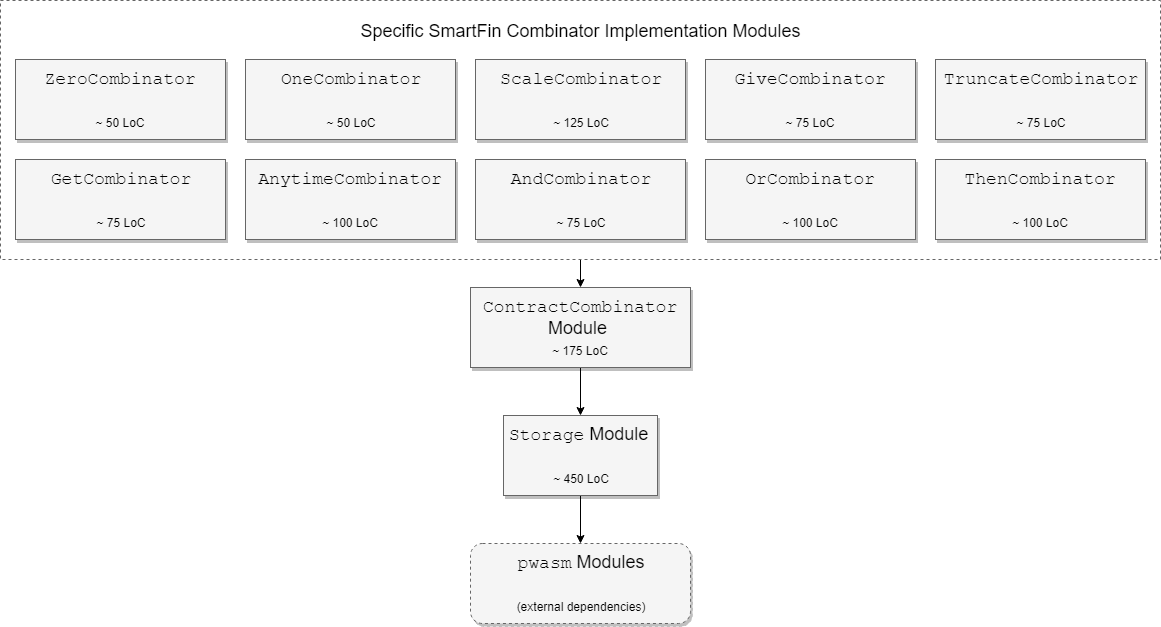
\includegraphics[width=\textwidth]{combinator-block.png}
    \caption{A dependency graph of the modules implemented to represent the SmartFin combinator semantics, with their approximate \textit{Lines of Code} (not including tests). \texttt{pwasm} modules are external dependencies, described in section \ref{smart-contract-tech}. The \texttt{Storage} module is described in section \ref{storage}.}
    \label{fig:combinator-block}
\end{figure}


\section{Designing a Programmatic Representation of SmartFin Combinators} \label{combinators-design}

\subsection{General Representation of Combinators}

As described in chapter \ref{combinator-DSL}, SmartFin is functional and compositional by definition. In any proposed smart contract implementation of SmartFin, representing the combinators in a functional manner is not simple; the smart contract must keep track of state over time, and individual combinators will have different state to keep track of. This suggests that a purely functional representation of the combinator behaviour may not be ideal, as keeping track of state could be complicated and unwieldy. \\

Furthermore, each combinator's functionality cannot be described simply as a single function - for example, how can we represent the \texttt{get} combinator, which acquires its sub-combinator at its horizon, without scheduled callbacks (which aren't possible within Ethereum smart contracts)? It makes more sense to represent it with an acquisition function and an \texttt{update} function which is called at a later date. \\

Due to the requirements of keeping track of state, and declaring multiple functions over this state, it would make sense to represent the combinators as classes rather than functions. As such, each combinator has a struct and a trait implementation. Due to the modular nature of the combinators in SmartFin, the information each combinator requires about their sub-combinators is minimal - there are no cases where certain combinations of combinators have non-standard behaviour. Because of this, the combinators implement a standard trait (\texttt{ContractCombinator}) for their functionality. \\

While the combinators cannot be easily represented in a smart contract in a functional manner, this does \textit{not} mean that they cannot be represented in a \textit{compositional} manner. In SmartFin, combinators may have a number of sub-combinators; this can represented as a tree of combinator objects, where each object may have zero, one, or two sub-combinator objects. This would be simpler than using some other data structure (e.g. a vector) to store the combinators, as it removes any extra requirements of external knowledge; each combinator object will only know about its sub-combinator objects, and nothing else. It also makes logic for traversal by recursion simple, intuitive, and efficient. \\

In summary, the final design for the representation of SmartFin's combinators in the smart contract is a tree of objects. Each object is a struct which implements the \texttt{ContractCombinator} trait, allowing combinators to call methods on sub-combinators without knowing which combinators they represent. Each combinator will store its own sub-combinators in its struct, and method calls will be propagated by recursive calls to the sub-combinators. Each combinator's behaviour will be implemented entirely within its struct's method implementations. \\

To illustrate this idea, take the SmartFin version of the financial contract representing a European option from section \ref{example-contracts}, \texttt{get truncate <01/01/2020 00:00:00> or scale 500 one zero}; the representation of these combinators as a tree of struct instances is depicted in figure \ref{fig:euro-option-tree}. \\

\begin{figure}[h]
    \centering
    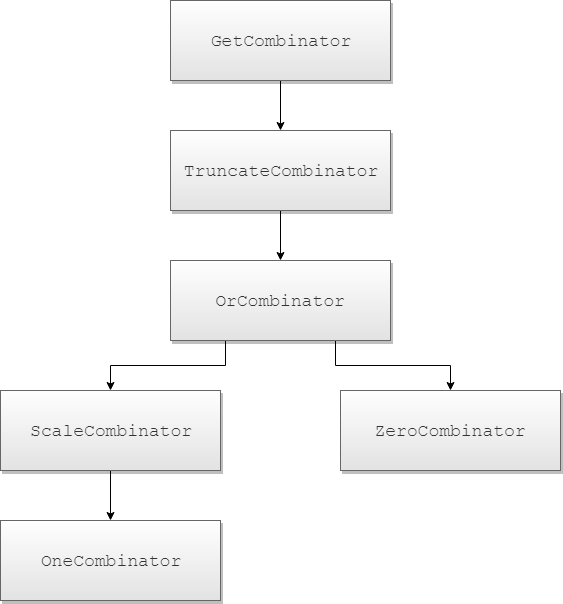
\includegraphics[width=0.7\textwidth]{euro-option-tree.png}
    \caption{The representation of the European option SmartFin contract, \texttt{truncate <01/01/2020 00:00:00> or scale 500 one zero}, as a tree of combinator struct instances.}
    \label{fig:euro-option-tree}
\end{figure}


\subsection{\texttt{ContractCombinator} Methods} \label{contract-combinator-trait}

The \texttt{ContractCombinator} trait is a trait that all combinator structs implement, with methods that are required regardless of the combinator type. This enables combinators to call methods on their sub-combinators regardless of the sub-combinators' types, and the same for the top-level smart contract. These methods are as follows: \\

\begin{itemize}
    \item \texttt{get\_horizon}: returns the combinator's horizon as an \texttt{Option<u32>}, with the value \texttt{Some(<U\-NIX Epoch time>)} if a horizon exists, or \texttt{None} otherwise.
    \item \texttt{past\_horizon}: returns true if the given time (in UNIX Epoch time) is beyond the combinator's horizon.
    \item \texttt{acquire}: handles the acquisition of the combinator (and sub-combinators if applicable).
    \item \texttt{update}: handles updating the combinator to the current time, mainly to evaluate payments that occur since the last call to \texttt{update}. The method returns the amount of funds in Ether that the counter-party should have paid the holder in this period, as a signed 64-bit integer (where a negative result signals payments from the holder to the counter-party).
    \item \texttt{get\_combinator\_number}: returns the combinator's enum value.
    \item \texttt{get\_combinator\_details}: returns a \texttt{CombinatorDetails} struct, containing the combinator's acquisition time as an \texttt{Option<u32>}, and whether or not it has been fully-updated as a \texttt{bool} (i.e. further calls to \texttt{update} will have no effect). These details can be used by parent combinators, or by the top-level smart contract - i.e. to check if the contract has concluded or been acquired.
    \item \texttt{serialize}: returns the combinator (and sub-combinators) in a serialized format (\texttt{Vec<i64>}), which is required to store the combinator tree in smart contract storage.
    \item \texttt{serialize\_details}: returns the combinator's \texttt{CombinatorDetails} struct in a serialized format (\texttt{Vec<i64>}), which is called when serializing the combinator. This is a trait method to provide a general implementation of this method, given that the \texttt{CombinatorDetails} objects have the same structure regardless of the combinator type, and all combinators implement the \texttt{get\_combinator\_details} method. \\
\end{itemize}

Besides these trait methods, each struct implementing \texttt{ContractCombinator} also implements a \texttt{deserialize} constructor. These are not present in the \texttt{ContractCombinator} trait because they are static - as there is no combinator object until after deserialization - and static methods cannot be defined for traits in Rust. This method takes in a vector representing the combinator tree, with all of its state, in a serialized format. It also takes in an index, which is the location of the combinator being deserialized in the vector. The method returns the deserialized \texttt{ContractCombinator} instance and the last index used during deserialization. The index is needed for combinators like \texttt{and}, where the starting index of the second sub-combinator is not known until the first sub-combinator is deserialized.


\section{Implementation} \label{combinator-implementation}

Every combinator has their own struct and implementation of the \texttt{ContractCombinator} trait, and the \texttt{ContractCombinator} module has some extra functionality for utility.


\subsection{The \texttt{ContractCombinator} Module}

The \texttt{ContractCombinator} module defines default implementations of some methods for the \linebreak\texttt{ContractCombinator} trait, as well as some utility methods.


\subsubsection{Default Method Implementations for the \texttt{ContractCombinator} Trait}

Default implementations are not provided for the \texttt{acquire}, \texttt{update}, and \texttt{get\_combinator\_number}, as these implementations obviously depend entirely on which combinator is being implemented. A default \texttt{get\_combinator\_details} method is also not implemented, as there is no way to declare that structs will have a specific member variable when implementing a trait (as opposed to something like a Superclass in other languages). As such, there is no way to obtain the \texttt{ContractDetails} struct from the member variable as far as the \texttt{ContractCombinator} trait is aware, and so each combinator struct must implement their own method to retrieve this variable. This is a specific limitation with Rust. In all combinators, the methods \texttt{get\_combinator\_number} and \texttt{get\_combinator\_details} have a trivial implementation, and so they are not mentioned further. \\

The default \texttt{get\_horizon} implementation returns \texttt{None}, as any combinators without sub-combina\-tors will have no horizon, and so it is the basest implementation of the method where no extra information about the combinator type is required. The default \texttt{past\_horizon} implementation gets the horizon with \texttt{get\_horizon}; if the horizon is \texttt{None}, then the horizon can never be passed, otherwise it is compared to the given time. This is never overridden by any \texttt{ContractCombinator} implementations, as it will never change as long as \texttt{get\_horizon} is accurate. \\

The default \texttt{serialize\_details} implementation pushes the combinator enum, the acquisition time (represented as the value, or -1 if no value exists), and whether or not the combinator is fully-updated (1 represents \texttt{true}, 0 represents \texttt{false}). These are obtained by the \texttt{get\_combinator\_number} and \texttt{get\_combinator\_details} functions. This is standard for all combinators, and is used in the \texttt{serialize} method. \\

The \texttt{serialize} method is required to store the combinator and its state in the smart contract storage between function calls, and serializes this information into a vector of signed 64-bit integers (or \texttt{i64}s). The default implementation of this method simply returns the return value of \texttt{serialize\_details}; this will represent any combinators with no extra state, and the other combinators will have to serialize their own state.


\subsubsection{Other Utilities in the \texttt{ContractCombinator} Module}

Besides the trait implementation, the \texttt{ContractCombinator} module also provides several utilities. One such utility is a \texttt{Combinator} enum representing the contract combinators defined in chapter \ref{combinator-DSL}, and implementations for converting between this enum and an integer (for serialization purposes). \\

The \texttt{CombinatorDetails} struct definition is also provided here, containing the acquisition time of a combinator, and whether or not a combinator is fully-updated. All combinators are able to return their \texttt{CombinatorDetails} struct; \texttt{fully\_updated} is used to prevent calling into combinators for no reason, and \texttt{acquisition\_time} is used to ensure that combinators have been acquired (especially \texttt{anytime} combinators) before being called into. Two methods for initialising a \texttt{CombinatorDetails} struct are also provided, one with default attributes (no acquisition time and not fully-updated), and one from the serialized format of the \texttt{CombinatorContract} struct. \\

The \texttt{ContractCombinator} module also provides two public functions for comparing times; \texttt{earliest\_time} will take in two times and return the value of the earliest, and \texttt{latest\_time} will take in two times and return the value of the latest. \\

The module also provides a function for deserializing combinators - given a serialized combinator vector and a starting index, the function will check the serialized combinator's enum and initialise a combinator object of the correct type using the correct \texttt{deserialize} constructor.


\subsection{Simple \texttt{ContractCombinator} Implementations}

Several of the \texttt{ContractCombinator} implementations have simple implementations throughout all of the combinator modules. The \texttt{get\_combinator\_number} method returns the value in the \texttt{Combinator} enum representing the implementing combinator's type. The \texttt{get\_combinator\_details} method just returns the \texttt{CombinatorDetails} object from struct. \\

\texttt{get\_horizon} typically returns \texttt{None}, or the latest horizon of any sub-combinators (except in the case of \texttt{truncate}). \texttt{serialize} will write the result of \texttt{serialize\_details} to a vector, followed by any struct variables, and then any sub-combinators sequentially. While it isn't on the trait, all combinators have a \texttt{deserialize} function which reads from a serialized vector as described and reconstructs the combinator struct. \\

Besides these methods, all combinators implement their own \texttt{acquire} and \texttt{update} methods as described below. All of these \texttt{acquire} methods will throw an error if the combinator is previously acquired or expired, and the \texttt{update} methods will return 0 balance change if the combinator is not acquired in the past or is fully updated.


\subsection{The \texttt{ZeroCombinator} and \texttt{OneCombinator} Modules}

The \texttt{acquire} method for both the \texttt{ZeroCombinator} and \texttt{OneCombinator}'s implementations of \texttt{ContractCombinator} both set the combinator's acquisition time to the current time. For the \texttt{update} method, both combinators mark themselves as fully-updated, \texttt{ZeroCombinator} returns 0 as the evaluated difference in balances, and \texttt{OneCombinator} returns 1.


\subsection{The \texttt{AndCombinator} Module}

The \texttt{acquire} method for the \texttt{AndCombinator} checks if the sub-combinators' horizons have passed yet. For each sub-combinator, if the horizon has not passed then its \texttt{acquire} method is called with the same parameters as the \texttt{AndCombinator}'s. The \texttt{AndCombinator}'s acquisition time is then set to the current time. \\

The \texttt{update} method calls \texttt{update} on the two sub-combinators in order. If both of the two sub-combinators are fully-updated after their \texttt{update} calls, then the \texttt{AndCombinator} is set as fully-updated. The sum of the values returned by the sub-combinators is returned.


\subsection{The \texttt{OrCombinator} Module}

The \texttt{OrCombinator} struct is one of the more complicated combinator implementations, requiring the holder to select which of its two sub-combinators should be acquired. The struct contains the combinator's \texttt{or} index. This is the index of the \texttt{or} combinator in the combinator contract, with regard to all \texttt{or} combinators, ordered sequentially by left-to-right occurrence and starting from 0. This is used to index into a vector of all \texttt{or} combinator choices in the contract, stored in the \texttt{Storage} struct described in section \ref{storage}. \\

A method \texttt{get\_or\_choice} is provided on the struct, which determines which sub-combinator should be acquired when the \texttt{or} combinator is acquired. The result is represented by an \texttt{Option<bool>} value, where \texttt{Some(true)} represents the first sub-combinator, \texttt{Some(false)} the second, and \texttt{None} that neither sub-combinator should be acquired. If either sub-combinator is expired, a value signalling that the other should be acquired is returned. If neither is expired, the \texttt{or} choice is looked up and returned from storage. \\

The \texttt{acquire} uses \texttt{get\_or\_choice} to check which sub-combinator to acquire. If \texttt{Some(val)} is returned then the relevant sub-combinator's \texttt{acquire} method is called and the \texttt{OrCombinator}'s acquisition time is set to the current time, otherwise nothing occurs. \\

The \texttt{update} method obtains the \texttt{or} choice by calling \texttt{get\_or\_choice} with the \texttt{OrCombinator} instance's \textit{acquisition} time, \textit{not the current time}. If the sub-combinator to have acquired is ambiguous, the method returns 0. If a concrete \texttt{or} choice is returned, the method checks if the relevant sub-combinator has been acquired; if not, then its \texttt{acquire} method is called with the \texttt{OrCombinator}'s \textit{acquisition} time. After this check, the \texttt{update} method on the relevant sub-combinator is called and returned, and the \texttt{OrCombinator} is set to fully-updated if the relevant sub-combinator is also fully-updated.


\subsection{The \texttt{GiveCombinator} Module}

The \texttt{acquire} method simply acquires the sub-combinator and sets the acquisition time. \texttt{update} simply updates the sub-combinator and returns the negated result. The combinator's fully-updated flag is set to the value of the sub-combinator's fully-updated flag.


\subsection{The \texttt{ScaleCombinator} Module}

The \texttt{ScaleCombinator} is one of the more complicated combinator implementations. This is because a \texttt{scale} combinator scales the sub-contract's value by an observable. This observable can be a fixed constant, or it can be a value that varies over time. Both cases must be handled by this combinator. The \texttt{ScaleCombinator} struct has a scale value, an \texttt{Option<i64>} that represents the \texttt{scale} combinator's observable when it is a constant value.  The struct also has an observable index, an \texttt{Option<usize>} representing the \texttt{scale} combinator's observable's index in a set of time-varying observable values. One of the scale value or observable index must have a concrete value, i.e. \texttt{Some(v)}, and the other must have no concrete value, i.e. \texttt{None}. \\

The method \texttt{get\_scale\_value} is implemented on the \texttt{ScaleCombinator} struct. This method checks if a concrete scale value exists; if so, it is returned, otherwise the observable index is looked up through the \texttt{Storage} struct and returned (as an \texttt{Option<i64>} which may not yet have a concrete value). If neither a concrete scale value or observable index exists, an error is thrown. \\

The \texttt{acquire} method is simple, simply acquiring the sub-combinator and setting the acquisition time. The \texttt{update} method gets the scale value using \texttt{get\_scale\_value}. If no concrete scale value exists yet then the value 0 is returned, otherwise the sub-combinator is updated, and fully-updated is set if the sub-combinator is fully-updated. The sub-combinator's update value is then multiplied by the scale value and returned.


\subsection{The \texttt{TruncateCombinator} Module}

The \texttt{CombinatorContract} implementation for the \texttt{get\_horizon} implementation returns the earliest of the \texttt{TruncateCombinator}'s truncated horizon and the sub-combinator's horizon - as described in section \ref{DSL-semantics}. The \texttt{acquire} method simply checks the horizon as usual, acquires the sub-combinator, and sets the acquisition time. \texttt{update} performs the usual call-through to the sub-combinator, setting fully-updated to the sub-combinator's fully-updated value and returning the result from \texttt{update} on the sub-combinator.


\subsection{The \texttt{ThenCombinator} Module}

The \texttt{acquire} method checks if the current time is past the first sub-combinator's horizon. If not, the first sub-combinator is acquired, otherwise the second is acquired, and then the acquisition time is set. The \texttt{update} method checks if the \texttt{ThenCombinator}'s acquisition time is past the first sub-combinator's horizon (as before). If not, the first sub-combinator is updated, otherwise the second is updated. Fully-updated is then set based on the sub-combinator, and the sub-combinator's update value is returned.


\subsection{The \texttt{GetCombinator} Module}

The \texttt{GetCombinator} struct is another relatively simple \texttt{ContractCombinator} struct, although it may seem unintuitive at first. The \texttt{acquire} method carries out the main behaviour of the \texttt{get} combinator. The sub-combinator's horizon is checked, and if a concrete horizon is found then the sub-combinator is acquired \textit{with the horizon as the acquisition time}. This will cause the sub-combinator to only become updated once the horizon is reached or passed, as is required by the definition of the \texttt{get} combinator in section \ref{DSL-semantics}. The \texttt{update} method is simple, calling through to the sub-combinator and setting fully-updated and returning the sub-combinator's \texttt{update} result as usual.


\subsection{The \texttt{AnytimeCombinator} Module}

The \texttt{AnytimeCombinator} is one of the more complex combinators, allowing the acquisition of the sub-combinator at any point until its horizon (as described in section \ref{DSL-semantics}). The \texttt{AnytimeCombinator} struct has an \texttt{anytime} index. This is the index of this \texttt{anytime} combinator's sub-contract acquisition time, in a vector of \texttt{anytime} acquisition times stored in smart contract storage. \\

The vector contains \texttt{(bool, Option<u32>)} tuples - the boolean value represents whether or not the corresponding \texttt{anytime} combinator has been acquired, and the \texttt{Option<u32>} represents the prospective acquisition time of the sub-combinator. If this time is in the future, it can be changed by calling the \texttt{acquire\_anytime\_sub\_contract} method on the smart contract's ABI, setting it to the current time as long as the parent \texttt{anytime} combinator has been acquired. If the prospective acquisition time is in the past, then it cannot be changed. \\

The \texttt{acquire} method sets the \texttt{AnytimeCombinator}'s acquisition time and sets the prospective acquisition time of the sub-combinator in the stored \texttt{anytime} acquisition times vector to the sub-combinator's horizon. This means that the sub-combinator can be acquired manually up until its horizon, after which its acquisition time will be locked in as the horizon. We cannot call \texttt{acquire} in this method on the sub-combinator, as a combinator can only be acquired once and the sub-contract's acquisition time may change in the future. \\

The \texttt{update} method checks if the sub-contract has been acquired yet. If not, then the \texttt{anytime} acquisition times vector is checked for its prospective acquisition time. If the sub-combinator's acquisition time has passed then \texttt{acquire} is called on it. After this, \texttt{update} calls through to the sub-combinator as usual.


\section{Evaluation} \label{combinators-eval}

In order to evaluate the representation of the SmartFin combinators in the implemented smart contract, the design of the combinators' representation in the smart contract can be qualitatively evaluated, and automated testing can provide some quantitative evaluation of their correctness.


\subsection{Combinator Representation}

Representing the combinators as a tree of \texttt{ContractCombinator} structs results in an intuitive composition of combinators that behave as one would expect based on the SmartFin contract definition. Combinators apply behaviours over their sub-combinators, and then call through to the sub-combinators; a financial contract written in SmartFin would also apply behaviour and propagate acquisition to sub-combinators, and so this representation is a natural fit. \\

One potential implementation approach that may also seem like a natural fit is the implementation of each combinator as its own smart contract. This would allow a SmartFin contract written to be represented as a set of linked smart contracts. Calling methods on each smart contract would call through to the sub-combinator's smart contract. This may seem like a closer match to SmartFin's semantics, as any financial smart contracts would be able to become sub-contracts for other financial smart contracts. There are a few issues with this design, however. One issue is that either state would have to be replicated across every smart contract (e.g. the holder and counter-party address), or it would have to be passed across smart contract boundaries with every function call, which would become difficult to implement in a trustworthy manner (e.g. verifying that the holder is correct). Another issue is that traditional financial contracts are a "package deal" - either you acquire the whole contract, or none of it. Representing each combinator as a smart contract could make it difficult to prevent any combinator in the financial contract being acquired without its parents. Circumventing this would require some path representing the parent-child relationship between combinators to be marked through the smart contracts, somewhat defeating the purpose of this representation. Gas costs of deploying large financial smart contracts would also be much higher with multiple smart contracts. For these reasons, using a single smart contract to represent a SmartFin contract is preferable.


\subsection{Design of the \texttt{ContractCombinator} Trait}

On the whole, the design of the \texttt{ContractCombinator} trait facilitated the operation of the combinators fairly well, and the chosen methods make contract acquisition/updating simple in general. The ability to get a combinator's horizon, or check if a time is past its horizon, is effectively used by every combinator with sub-combinators; as such, the \texttt{get\_horizon} and \texttt{past\_horizon} methods are a useful part of the trait. The ability to serialize combinators relatively painlessly with \texttt{serialize\_details} and the guaranteed \texttt{serialize} method allowed the serialization of the combinators to operate intuitively and efficiently through recursion. Unfortunately, the trait did not provide such methods for deserialization as there can be no static methods defined on a trait. As such, the \texttt{deserialize} constructor was implemented on each combinator struct - this is a limitation of Rust. \\

Another slight issue with the \texttt{ContractCombinator} trait is the \texttt{get\_combinator\_details} and \texttt{get\_combinator\_number} methods. Every combinator has an implementation of these methods, despite the fact that the implementations are extremely similar. Both of these methods could be implemented on the \texttt{ContractCombinator} trait easily if there were a way to require the \texttt{ContractCombinator}-implementing structs to have certain member variables (like a Superclass); unfortunately, Rust does not provide such a mechanism, and so every struct must implement a method for this. Both methods are required to obtain information needed for serialization and for acquisition/updating the contract, so the current solution is currently the best option available in Rust. \\

Some possible changes that could be made to \texttt{ContractCombinator} involve defining more getter functions, including a function that would return a vector of sub-combinators (which would have 0, 1, or 2 elements). This would allow default implementations of many of the simpler methods in the \texttt{ContractCombinator} trait which typically call through to the sub-combinators, e.g. \texttt{get\_horizon} and \texttt{serialize}. Overall, this could potentially reduce the amount of repeated code required between the combinator implementations. Unfortunately, as mentioned already, there is no way to require the definition of a member variable on a struct implementing a trait in Rust. This means that instead of writing repeated implementations for \texttt{get\_horizon} and other simple methods, there would be more repetition of these getter functions. Unless some method of requiring struct members is implemented in Rust, the benefits to such a change would thus be minimal, hence why they went unimplemented. \\

While the recursive behaviour of the \texttt{acquire} method is a natural fit for the combinators, one possible issue with this design is that the expected behaviour of acquiring the SmartFin combinators has been split across two different methods - \texttt{acquire} and \texttt{update}. For example, typically acquiring the \texttt{one} combinator would result in a payment occurring from the counter-party to the holder; with the current implementation, acquiring the \texttt{one} combinator records no payments until \texttt{update} is called. This is more of a ramification of the design of the smart contract ABI than a direct design decision; the \texttt{update} method is implemented to keep track of payments over time, whereas the \texttt{acquire} method simply exists to denote acquisition times. Furthermore, the smart contract ABI updates the balance of the contract in its \texttt{acquire} method, nullifying this issue from any external point-of-view. Besides this, the need for an \texttt{update} method is obvious given the lack of scheduled callbacks/persistent operation of the smart contract, as explained in section \ref{contract-design}. These reasons justify the compromise of separate \texttt{acquire} and \texttt{update} methods.


\subsection{Design of the Combinators' Implementations}

Most of the combinators implement fairly trivial or straightforward behaviour, and as such there is little to discuss regarding their design. \\

The decided-upon implementation of the setting of observables' values is somewhat interesting. Due to the nature of Ethereum smart contracts, it is impossible to read observables' values from off-chain data. As such, the only way to obtain these values is to have them passed into the contract by an external user, or obtained from another smart contract (eventually requiring external user input). \\

In the definition of the original DSL by Peyton Jones et al.\cite{SPJ}, an observable is defined as something with a value that both the holder and counter-party would agree upon. This definition was considered for the setting of observables, leading to a design where both parties would need to provide a matching value for an observable to set its value. After a discussion with Dr. Panos Parpas of Imperial College London, who wrote financial contracts professionally in the past, this design was passed over in favour of letting a pre-defined arbiter set the value of an observable. This more closely matches the way that traditional financial contracts handle observables, where typically a pre-defined information source for the value of any observable will be included in the financial contract. This also prevents parties from lying about observable values to avoid unfavourable transactions - although, as described in \ref{contract-design}, it is impossible to bind the parties to a smart contract's terms without external tools.


\subsection{Testing}

In order to ensure that the combinator implementations behave correctly, extensive unit testing has been implemented to test the functionality of all structs implementing \texttt{ContractCombinator}. The tests follow the same structure for all combinators, but some combinators require extra tests. In total, there are 151 unit tests for the combinator modules, made up of ~2750 LoC. Besides the unit tests mentioned here, all combinators are tested in the Rust and JavaScript integration tests mentioned in section \ref{contract-testing}.


\subsubsection{\texttt{ContractCombinator} Module Tests}

The \texttt{ContractCombinator} module provided several utilities, for which unit tests have been written. The default implementations of the \texttt{ContractCombinator} methods were tested by implementing a \texttt{DummyCombinator} struct, which only implements methods with no default implementation. \\

The two time comparison methods, \texttt{earliest\_time} and \texttt{latest\_time}, are both tested with concrete values and \texttt{None} values for time. The methods for converting between the \texttt{Combinator} enum and integer values is tested for all of the enum values. The \texttt{serialize\_details} method is tested on the \texttt{DummyCombinator}, as well as the \texttt{serialize} implementation. The \texttt{deserialize\_combinator} method is tested by defining a combinator tree with all combinator types present and random state, and serializing it. This serialized tree is then deserialized and serialized again; if the second serialized vector is equal to the first, then the deserialization method works correctly - assuming that the serialization methods work correctly. The \texttt{deserialize_combinator} function is also tested with an empty serialized combinator vector, to ensure that the correct error is thrown.


\subsubsection{General Combinator Testing Methodology}

All of the combinators are unit-tested, mostly following the same testing methodology. For each combinator, the \texttt{get\_combinator\_number} and \texttt{get\_horizon} methods are tested. For combinators with sub-combinators, all variations of sub-combinator horizons are tested, e.g. first sub-combinator's horizon is later, second is later, both are undefined, etc. \\

The \texttt{acquire} method is also checked to ensure that it sets the \texttt{CombinatorDetails} struct's acquisition time member correctly, and \texttt{update} is checked to ensure that the struct's fully-updated flag is set when required. The value returned by calling \texttt{acquire} and then \texttt{update} is checked in all permutations (e.g. expired, non-expired, one sub-combinator expired, etc.). The \texttt{update} method is tested before \texttt{acquire} is called, or before the acquisition time is reached, to ensure that it does nothing. \\

The \texttt{serialize} method is testing by ensuring that all relevant information is encoded in the serialized combinator vector, where the combinator implements extra serialization beyond the default implementation. The \texttt{deserialize} constructor is tested by serializing, deserializing, and re-serializing the combinator (as with the \texttt{ContractCombinator} tests). Any errors which should be thrown are also tested. This covers the basic operation of all combinators, and only a few combinators require extra testing beyond this.


\subsubsection{Specific Combinator Tests}

The \texttt{OrCombinator} implementation is tested with the left and right sub-combinators chosen or expired for every testing scenario, as well as several tests where no choice is made yet. The implementation is also tested to ensure that behaviour remains consistent, i.e. you cannot choose one sub-combinator and then see the results of the other sub-combinator after updating. \\

The \texttt{ScaleCombinator} implementation is tested with constant scale values, defined observables, and undefined observables. It is also tested without either is set, to ensure that an error is thrown. \\

The \texttt{AnytimeCombinator} implementation is tested to ensure that acquisition of the sub-combinator occurs on calls to \texttt{update}, and that this is set to the horizon correctly. The \texttt{update} method is also tested by simulating acquisition of the \texttt{anytime} sub-contract, to ensure that it is acquired at the correct time, and that the value returned is correct. Tests with various combinations of acquisition and updating are implemented to ensure correctness and consistency of the acquisition/payment evaluation behaviour. It is also checked that the \texttt{AnytimeCombinator} throws the correct error when the \texttt{anytime} sub-contract acquisition time is before the parent \texttt{AnytimeCombinator}'s acquisition time.


\subsection{Conclusion}

Overall, the combinators' behaviour seems to follow the specification described in section \ref{DSL-semantics} based on the thorough unit and integration testing. The design is relatively representative of the SmartFin combinators, although some compromises had to be made due to the nature of smart contracts (like separate \texttt{acquire} and \texttt{update} methods). The design of the \texttt{ContractCombinator} trait covers all of the required functionality, and allows combinator implementations to be relatively simple on the whole.


\section{Remarks}

This chapter has described how SmartFin's combinators are represented in the implemented smart contract. The final result of this and the previous chapters is a smart contract implementation which can represent any given SmartFin contract, with minimal concessions made due to the nature of smart contracts. \\

While this is useful, we are still missing easy ways of creating, deploying, evaluating, and interacting with financial smart contracts; the next chapter will describe the web client created for this purpose.


\chapter{The Financial Smart Contract Web Client} \label{web-client}

One desired benefit of this project's contributions is the simplification of the creation of financial contracts. While the implementation of the financial smart contract program does simplify this, it is difficult to interact with due to the heavy serialization required in the smart contract's ABI. Rather than requiring users to learn and implement serialization/deserialization of all function parameters and return values, a web client has been implemented to facilitate this interaction and provide some additional functionality. \\

The web client facilitates the composition, deployment, and interaction/monitoring of financial smart contracts, as well as some basic evaluation functionality - a feature provided to reduce the risk of writing financial contracts and smart contracts. This chapter will describe the design and implementation of this web client. The implemented modules discussed in this chapter are depicted as a dependency graph in figure \ref{fig:client-block}. \\

\begin{figure}[h]
    \centering
    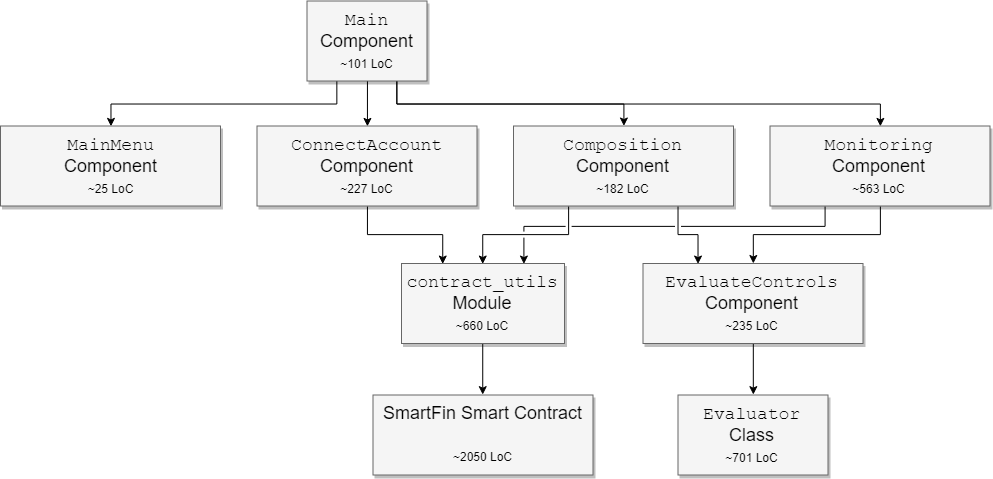
\includegraphics[width=\textwidth]{client-block.png}
    \caption{A dependency graph of the modules implemented for the web client, with their approximate \textit{Lines of Code} (not including tests). Small UI and data classes are not depicted. The SmartFin smart contract is described in chapters \ref{smart-contract-impl} and \ref{combinators-main}.}
    \label{fig:client-block}
\end{figure}


\section{The Design of the Web Client}

\subsection{Architecture}

From the beginning, the web client was designed around the use of \textit{React}\cite{react} - a JavaScript UI framework. Using some framework was effectively a necessity in order to design the web client with some semblance of structure, and pure HTML and JavaScript would be significantly harder to coordinate. React was partly chosen due to its relative simplicity, but also due to previous development with it - these factors enabled rapid development of the web client. This is important as the web client UI is intended to be a more basic vessel for specific financial smart contract functionality, not an interesting technical product of its own right; as such, focusing too intently on the web client UI would not be the best use of time. \\

The design of the web client follows React's typical structure of designing UI views as components, which can be as large as an entire application, or as granular as a single label. Each component has certain \textit{properties} passed down by a parent component, and certain \textit{state} defined in its constructor. The properties and state are intended to act as a \textit{single source of truth}. Components also implement a \texttt{render} method, which returns the view described in an HTML-like language, \textit{JSX}. The \texttt{render} method does not alter state directly, to separate the view generation from the component behaviour. Besides this, Components can have several methods which may hook into UI lifecycle methods, UI interaction events, and so on. These methods define the behaviour of the component. \\

More intricate UI design architectures were also considered, such as the \textit{Model View View-Model} pattern. This pattern separates the data, UI, and behaviour into a model, view, and view-model respectively. The model and view are relatively straightforward, and the view-model maps the state stored in the model to information displayed in the view, and interaction events on the view to updates in the model. While this architecture is robust, it is relatively complex to implement, requiring at least two classes per UI view (the view and view-model). It also requires organising data into shared models, whereas the web client's different views will have relatively distinct sources of data - some will read from deployed smart contracts, others entirely from the UI. The increased complexity in implementing this kind of architecture was deemed unnecessary, as the typical React architecture is both sufficient and simple to write.


\subsection{Web Client Components}

Each screen of the application has its own component class, as well as some elements that are repeated throughout the web client on multiple views, and some that implement relatively complex behaviour. The main screens of the application are: \\

\begin{itemize}
    \item The \textit{connect} view, for connecting to a blockchain with an account. This is required so that financial smart contracts can be deployed to a blockchain, or interacted with if they are already deployed.
    \item The \textit{main-menu} view, for navigation between views.
    \item The \textit{composition} view, for composing and deploying financial smart contracts. Composed financial contracts can be evaluated here.
    \item The \textit{monitoring} view, for viewing the state of deployed financial smart contracts and interacting with them. Deployed financial smart contracts can be evaluated here. \\
\end{itemize}

The \textit{evaluation} view is also a major view, but it is shown in an overlay on the \textit{composition} and \textit{monitoring} views instead of having its own screen (to obtain a contract definition from these views). By selecting these as the main views of the web client, the major functionality which is required is neatly separated into one component per major function. The entire web client is always rendered within a \textit{main} view, which handles routing between the different views. The relationship between these views is depicted in figure \ref{fig:client-block}. \\

Other views with their own components include a view for choosing an \texttt{or} combinator's sub-contract, setting an observable's value, acquiring an \texttt{anytime} contract's sub-combinator, and staking and withdrawing Ether - all on a deployed financial smart contract. There are also components for selecting a time for the insertion of a UNIX Epoch time into a combinator contract, inputting a deployed contract's address, and displaying instructions for writing a combinator contract. There are several smaller UI components as well, for displaying animations or specially-formatted information.


\subsection{Other Functionality}

Besides the UI functionality, there are several other facets of the web client's functionality. Static functions for interacting with the blockchain and deployed financial smart contracts were implemented in a \texttt{contract-utils} module. Evaluation of financial contracts written using the combinator DSL is implemented in the \texttt{Evaluator} class. This is represented as a class as it enables pre-processing and step-by-step evaluation of a financial smart contract, setting \texttt{or} combinator choices and acquisition times incrementally as they are encountered, which requires state to store pre-processing results and evaluation progress. The design and implementation of the \texttt{Evaluator} class is described in more detail in section \ref{evaluator}.


\section{Implementation}

\subsection{Technologies}

As described earlier, the web client UI is implemented using \textit{React}\cite{react}. \textit{Web3.js}\cite{web3-intro}, a JavaScript implementation of the Ethereum API, is used to interact with Ethereum blockchains. \textit{Yarn} is used for package management. \textit{webpack}\cite{webpack} is used to run a development server, and build the production server files. \textit{Babel}\cite{babel} is used to allow the usage of JavaScript ES6 functionality with incompatible packages, mainly for nicer module import syntax/functionality. \textit{Sass}\cite{sass} is used to improve the structure of the UI styling, allowing the separation of styles into modules, and the definition of variables. \textit{Browserify}\cite{browserify} is used to allow node modules to run in the browser. \textit{Moment}\cite{moment} is used to handle conversion between date/time formats. \textit{Mocha}\cite{mocha} is used as a testing framework, for automated unit and integration tests.


\subsection{Contract Utility Functions}

In order to handle interaction with the blockchain, the \texttt{contract-utils} module was created. This module has function implementations for setting up the Web3 connection, serializing/deserializing financial smart contract information, calling smart contract functions, and more. Several data classes are also defined, to represent smart contract interaction results. The exported functions are implemented as follows: \\


\subsubsection{Financial Smart Contract ABI Functions}

All of the functions on the financial smart contract ABI have a function implementation in the \texttt{contract-utils} module, in order to provide an abstraction of the smart contract. Each of these functions is asynchronous, returning a \texttt{Promise} which will either \textit{resolve} or \textit{reject} in the future. If an error occurs, the \texttt{Promise} is rejected with a descriptive error message, otherwise the \texttt{Promise} resolves with the correct return value. These functions are implemented as follows:


\subsubsection{\texttt{getHolder, getCounterParty, getConcluded, getUseGas, getLastUpdated, getBalance}}

These getter functions are easily handled by simply calling the respective method on the provided smart contract object from the given address, and resolving the returned \texttt{Promise} with the result.


\subsubsection{\texttt{withdraw, stake, acquireContract, updateContract, setOrChoice, setObsValue, acqui\-reSubContract}}

Similar to the getter functions, these functions are implemented by calling the respective method on the given smart contract object from the given address, with all required parameters given through the function signature. The \texttt{Promise} is rejected if an error occurs, or resolved when the operation succeeds.


\subsubsection{\texttt{getOrChoices, getObsEntries, getAcquisitionTime}}

Similarly to the getter functions, these functions call the smart contract's respective method and await a result. Once a result is obtained, it must be deserialized before it can be returned. The implementation of the deserialization functions are described in section \ref{ABI-pure}. \\

For \texttt{getOrChoices} and \texttt{getAcquisitionTimes}, the returned serialized vector of bytes is processed into an array of \texttt{Option} objects - a class implemented to represent Rust's \texttt{Option<T>} objects, with similar functionality. \\

The \texttt{getObsEntries} function obtains a list of observable entries from the contract method result - i.e. the arbiter addresses, values, and names of each observable - in a serialized form. An array of \texttt{ObservableEntry} objects is returned, a class that contains these three properties of an observable as well as its index. For each observable entry, the first 4 elements of the serialized vector are deserialized using the \texttt{deserializeAddress} method, an \texttt{Option} is deserialized from the following element(s), and then the name is deserialized from the following elements with \texttt{deserializeName}.

\subsubsection{\texttt{getCombinatorContract}}

\texttt{getCombinatorContract} similarly calls its respective method on the given smart contract, and deserializes the result into a human-readable combinator contract string. The serialized array is processed recursively; the first element being deserialized is converted into a combinator string, and then the following elements are deserialized based on the combinator's type. \\

\texttt{zero} and \texttt{one} can be returned immediately. \texttt{and}, \texttt{or}, and \texttt{then} all deserialize the following two sub-contracts, and then return their combinator joined with the two sub-contracts. \texttt{give}, \texttt{get}, and \texttt{anytime} can do the same, but for only one sub-contract. \texttt{truncate} takes the second element as a UNIX Epoch time and converts it into a human-readable time, followed by the deserialized sub-contract. \\

In the case of the \texttt{scale} combinator, the second element is used to indicate whether a constant or time-varying observable is present; if the value is constant it is simply added to the contract, otherwise the following elements are deserialized as an \texttt{ObservableEntry} (as for \texttt{getObsEntries}). Following this, the sub-contract is also deserialized.


\subsubsection{Other Utility Functions} \label{contract-util-functions}

Besides the abstraction of the financial smart contract ABI, the \texttt{contract-utils} module provides some extra utility functions for dealing with blockchain interaction.

\subsubsection{\texttt{setupWeb3}}

This function initialises the \textit{Web3} instance, which allows the web client to communicate with Ethereum blockchains. The function takes in a flag for whether or not to connect to \textit{MetaMask}, a Google Chrome extension for managing blockchain accounts, as well as an optional blockchain URL. In order to initialise the Web3 instance, a provider must be obtained; the Web3 instance communicates with the blockchain through a provider. If using MetaMask, the Web3 provider is obtained from the browser window, otherwise an HTTP provider is initialised with the passed in blockchain URL. The Web3 instance is then initialised, or if already initialised its provider is reset.

\subsubsection{\texttt{unlockDefaultAccount}}

This function sets and permanently unlocks the default account for testing, using the Parity blockchain client's default testing account. This is only used for testing, \textit{not} in production.

\subsubsection{\texttt{unlockAccount}}

This permanently unlocks the given address' account with a given password. This is used when providing a blockchain/account manually, which should only be used when security is not an issue. When security matters, MetaMask should instead be used.

\subsubsection{\texttt{loadAndDeployContract}}

This function deploys a financial smart contract to the connected blockchain. This is done by importing the financial smart contract code and ABI from another JavaScript module (set up as part of the smart contract build process), which are then used as parameters for a smart contract deployment transaction. The gas cost of deploying this smart contract is estimated and the smart contract transaction is deployed. The result of deployment is relayed asynchronously through a \texttt{Promise} object.

\subsubsection{\texttt{serializeCombinatorContract}}

This function is used to serialize a human-readable combinator contract, so that it can be passed across the financial smart contract ABI in the form of a vector of integers. It takes a combinator contract string and iteratively processes each combinator. For the majority of combinators, the combinator's numeric representation can simply be looked up and inserted into the serialized array, thanks to the simple compositional syntax of the DSL (see section \ref{DSL-BNF}). \\

For the \texttt{truncate} combinator, the date needs to be serialized. If the date is given in UNIX Epoch format, then it can simply be verified and pushed onto the serialized array. If the date is given in a human-readable form, then it is parsed using the \textit{Moment} package and converted into UNIX Epoch time. \\

For the \texttt{scale} combinator, the observable must be parsed. If a constant scale value is provided, the number 1 followed by the scale value is pushed. If a name and address are present, then the number 0 is pushed and the serialized address and name must be pushed onto the serialized array. The address is serialized by \texttt{serializeAddress}, which converts the address string into four signed 64-bit integers. The name is serialized by \texttt{serializeName}, which simply converts a string into an array of character codes by mapping, with the length of the name at the head.

\subsubsection{\texttt{verifyContract}}

The function \texttt{verifyContract} will take in a combinator contract string and verify that the syntax is correct. There is no semantic verification required, as the combinator DSL does not have any semantic restrictions. \texttt{verifyContract} recursively verifies the contract syntax, returning an object containing either a \texttt{VerificationError} or the index at which the contract terminates. The \texttt{VerificationError} class allows the definition of an error with an error stack, to aid debugging in the contract composition view. \\

In the \texttt{verifyCombinator} helper function, the contract atoms are processed recursively. If a sub-contract returns an error, then the current atom's information is added to the error stack. \texttt{zero} and \texttt{one} can simply return the termination index. \texttt{give}, \texttt{get}, and \texttt{anytime} all return the verification of their sub-contracts, and \texttt{and}, \texttt{or}, and \texttt{then} similarly verify the two sub-contracts. \\

For the \texttt{truncate} combinator, the time must be verified. If the given time is not an integer, then it is verified as a human-readable date of the form \texttt{`<DD/MM/YYYY HH:mm:ss( ZZ)?>'}, i.e. a date, time, and optional time zone. If the date format is incorrect, an error is thrown, otherwise it is converted into a UNIX Epoch time integer. If the time is an integer, it is verified to ensure that it fits within the bounds of an unsigned 32-bit integer. \\

The \texttt{scale} combinator can have a constant or time-varying scale value. If a constant scale value is found, it is checked that it fits within the bounds of a signed 64-bit integer. If a name and address are found, then the address is checked with \texttt{Web3.utils.isAddress}.

\subsubsection{\texttt{isSmartContract}}

This function takes an address and returns true if a smart contract exists with that address on the connected blockchain. To do this, the \texttt{Web3.eth.getCode} function is called to get the smart contract code associated with the given address. If any errors occur or no code is returned, the address is not a smart contract address.

\subsubsection{\texttt{compareTime}}

This is a standard comparison method which takes two times and returns 1, 0, or -1. \texttt{undefined} is treated as larger than any numerical value - this is because a financial contract with an undefined horizon is treated as if it expires later than a financial contract with a defined horizon. \\ \\


\subsection{Main View}

The \textit{main} component contains all other components rendered in the web client, and handles routing between them. Its state contains the Web3 instance, the current financial smart contract instance (if one exists), the current account address (if it exists), the application state, and an \texttt{Evaluator} object. The Web3 instance, smart contract instance, account address, and \texttt{Evaluator} instance are all passed down to the view currently being rendered. These views implement the behaviour which relies on these values. \\

The initial view is the blockchain connection view. A function is passed to the \texttt{ConnectAccount} component, which implements the connect view, to set the Web3 instance and account address. When this function is called, the main state is updated and the application state is changed to \texttt{`main-menu'}. This allows the application state to transition to the main-menu once the blockchain details are obtained. \\

The \texttt{MainMenu} component is given two functions as properties, one transitioning to the composition view, the other transitioning to the monitoring view. These functions update the main state to set the application state to the respective views when called, and are used to implement navigation buttons. \\

Both the \texttt{Composition} and \texttt{Monitoring} components are rendered within a container, wrapped with a back button which updates the application state to \texttt{`main-menu'}. This allows navigation between these two views and the main-menu view.


\subsection{Blockchain Connection View}

The first major view a user reaches in the web client is the blockchain connection view, shown in figure \ref{fig:connect}. This view allows the user to connect to a blockchain via MetaMask, or by manually inputting the blockchain and account details. \\

\begin{figure}[h]
    \centering
    \adjincludegraphics[trim={{.2\width} {.35\height} {.2\width} {.1\height}},clip,width=\textwidth]{connect.png}
    \caption{The blockchain connection view, used to connect to a blockchain.}
    \label{fig:connect}
\end{figure}

This view is comprised of a button to connect to MetaMask, or several inputs for manually inputting blockchain data. When the MetaMask connection button is pressed, \texttt{setupWeb3} function from the \texttt{contract-utils} module is called with a MetaMask flag. This attempts to obtain the Web3 details from the browser; if successful, the application will update the main state and progress to the main-menu view, otherwise an error is displayed. \\

In order to manually connect to a blockchain, the blockchain URL must be input to the given input (defaulting to the typical local blockchain address) and a button must be pressed. This will also call \texttt{setupWeb3}, this time with the given blockchain URL. If the URL cannot be connected to, then an error is displayed, otherwise an address/password input is displayed. Once input, pressing the button will attempt to unlock the account with the \texttt{unlockAccount} function from \texttt{contract-utils}. If successful, the view will progress to the main-menu, otherwise an error is displayed. \\

While connecting to the blockchain, it is possible that silent failure will occur. To catch this, the \texttt{ConnectAccount} component will register a timeout on every asynchronous call to the blockchain for 10 seconds. If this timeout is reached, then an error is displayed and the connection is assumed to be unsuccessful. The Web3 instance is discarded, and the view reverts to its initial state (with extra error state).


\subsection{Main-Menu View}

The main-menu view is a simple view which displays two buttons, as shown in figure \ref{fig:main-menu}. Each button's click event handler is registered to a function passed down from the parent view as a property. One button navigates to the composition view, the other to the monitoring view. \\

\begin{figure}[h]
    \centering
    \adjincludegraphics[trim={{.2\width} {.3\height} {.2\width} {.3\height}},clip,width=\textwidth]{main-menu.png}
    \caption{The main-menu view, used to navigate throughout the client.}
    \label{fig:main-menu}
\end{figure}


\subsection{Contract Composition View}

The contract composition view displays a text-area input and some buttons, as shown in figure \ref{fig:composition}. The text-area input receives a combinator contract, and the option buttons allow the user to view combinator DSL instructions, insert a UNIX Epoch time into the text-area input, and evaluate or deploy the composed contract. \\

\begin{figure}[h]
    \centering
    \adjincludegraphics[trim={{0\width} {.2\height} {0\width} {.07\height}},clip,width=\textwidth]{composition-empty.png}
    \caption{The composition view, used to compose SmartFin contracts and deploy their corresponding smart contracts.}
    \label{fig:composition}
\end{figure}

The combinator contract is stored in the \texttt{Composition} component's state, and updates every time the text-area input's value changes. All of the buttons will open a \textit{modal} component, i.e. a view displayed in an overlay over the current view. Whether or not each modal is visible is represented in the \texttt{Composition} component's state as a flag. Error messages/warnings are also stored in the state. \\

Upon pressing each button, the respective modal is opened. The modals contain a button to close themselves, which calls a \texttt{closeModal} function passed in as a property. The \textit{help} modal is fairly trivial, and the \textit{evaluate} modal renders an \texttt{EvaluateControls} component described in section \ref{client-evaluate}. The \textit{input UNIX time} modal contains a \texttt{TimeSelect} component, which has a date and a time input, and sets state variables to reflect their value. The selected time is returned through a callback property. The time is then inserted into the text-area by getting the cursor location, splitting the contract at this location, inserting the time, and rejoining the contract. \\

The \textit{deploy contract} modal contains a \texttt{DeployControls} component, which takes the combinator contract, the current address, a warning, and a callback for the deployed contract. Pressing the button to display the modal will first call \texttt{verifyContract}; if the contract is not valid, a descriptive error is displayed, otherwise the deploy modal is opened. The \texttt{DeployControls} component takes a holder address and a use-gas checkbox, and deploys the contract with the \texttt{loadAndDeployContract} function. The contract is returned with a callback property, which updates the main state with the deployed smart contract object.


\subsection{Contract Monitoring View}

The contract monitoring view is implemented in the \texttt{Monitoring} component, displaying a financial smart contract's state and allowing the user to interact with it, as shown in figure \ref{fig:monitoring}. When the view is entered, it will obtain the state of the financial smart contract instance currently stored in the main state, passed down as a property, using the getter functions from \texttt{contract-utils}. If no contract exists in state yet, an error is shown. \\

\begin{figure}[h]
    \centering
    \adjincludegraphics[trim={{.15\width} {.1\height} {.15\width} {.11\height}},clip,width=\textwidth]{monitor-one.png}
    \caption{The monitoring view, used to monitor and interact with deployed financial smart contracts.}
    \label{fig:monitoring}
\end{figure}

The user can press the \textit{load contract} button to open a modal with a contract address input, which calls \texttt{getContractAtAddress} and returns the contract instance to the main state through a callback property. When the \texttt{Monitoring} view receives a new contract instance, it will attempt to read the state from the contract again. If any getter functions fail, an error is shown indicating that the smart contract may not be a compatible financial smart contract. Financial smart contract state is re-obtained every few seconds, registering a new timeout every time it's checked. \\

Besides displaying contract state, the \texttt{Monitoring} component has several buttons/modals for interacting with the financial smart contract. These all open modals containing components with simple inputs for the financial smart contract method parameters. These inputs are used to call the respective \texttt{contract-utils} method. The inner modal component will then call a callback provided by the \texttt{Monitoring} component which closes any open modal and re-obtains the financial smart contract state. There is also a button to open an \textit{evaluate contract} modal, which is described in section \ref{client-evaluate}. \\


\subsection{Contract Evaluation} \label{client-evaluate}

The \textit{monitoring} and \textit{composition} view both allow the user to open a modal to evaluate a combinator contract. This displays an \texttt{EvaluateControls} component, which lets the user step-through a financial smart contract and evaluate the final value, depicted in figure \ref{fig:eval-scale-obs-evaluated}. While stepping through the contract, the user must provide acquisition times and choices for \texttt{or} combinators. The final value is represented as a sum of products of constant values and time-varying observable names, for more details see the user manual at appendix \ref{appx:user-manual}. \\

\begin{figure}[h]
    \centering
    \adjincludegraphics[trim={{.15\width} {.28\height} {.15\width} {.23\height}},clip,width=\textwidth]{eval-scale-obs-evaluated.png}
    \caption{The \textit{Evaluation} menu, after evaluating a SmartFin financial contract.}
    \label{fig:eval-scale-obs-evaluated}
\end{figure}


\subsubsection{The \texttt{Evaluator} Class} \label{evaluator}

An \texttt{Evaluator} class has been implemented order to maintain the state of step-through evaluation. This state is not just stored in the \texttt{EvaluateControls} component as it should persist across multiple views, and it keeps the \texttt{EvaluateControls} component mainly focused on the view. Furthermore, testing a pure JavaScript class is significantly easier than testing React components, and using automated testing for the \texttt{Evaluator} class is essential to thoroughly ensure that it operates correctly. \\

For context, the basic lifecycle of the \texttt{Evaluator class} is as follows: \\

\begin{enumerate}
    \item A SmartFin contract is provided through the \texttt{setContract} method.
    \item The contract is pre-processed with the \texttt{\_processCombinators} method, to store state that will be useful for evaluation (like a map of sub-contracts to horizons).
    \item The \texttt{hasNextStep} method is called to check if options must be set on the \texttt{Evaluator} before the SmartFin contract can be evaluated. If not, jump to step 7.
    \item The \texttt{getNextStepThroughOptions} method is called to return the current set of options that the user must choose between and input while stepping through the contract (either an acquisition time or an \texttt{or} choice).
    \item The \texttt{setStepThroughOption} method is called to input the chosen option.
    \item The \texttt{hasNextStep} method is called, and if it returns true then return to step 4.
    \item Once no more values must be input by the user for evaluation to be possible, \texttt{evaluate} is called to get the string representation of the value of the SmartFin contract with the current user input values. \\
\end{enumerate}

In order to describe the implementation of the \texttt{Evaluator} class, it is first necessary to describe how acquisition times are represented in step-through evaluation of a combinator contract.


\subsubsection{Representing Acquisition Times with Time Slices} \label{time-slices}

When a combinator contract is acquired, the acquisition time will affect its value. For this reason, it is necessary to decide any relevant acquisition times in a combinator contract before it can be evaluated. One way to do this would be to have the user simply input any time, but it is possible to do better. In order to evaluate the contract we aren't really interested in \textit{any} time, but only in several discrete segments of time in which the value of the contract is fixed - i.e. \textit{time slices}. \\

For example, consider the contract \texttt{one}. Acquiring this contract at any time will result in the value 1 Wei being obtained, and so the acquisition time does not affect the value of the contract. This contract has \textit{one} time slice. Now take the contract \texttt{truncate 10 one} - this contract has the value 1 Wei if acquired before the time 10, and 0 Wei if acquired after 10. As such, there are \textit{two} time slices we are interested in, 0 to 10 and 11 to the end of time. As such, the user can evaluate the contract just by providing the time slices in which the contract will be acquired, instead of an exact time. This shows the user which distinct time periods are important, and allows acquisition times to be assumed when only one time slice exists. \\

In order to calculate the time slices in which a contract's value is fixed, the contract can be recursively evaluated. The combinators \texttt{zero} and \texttt{one} have a single time slice from 0 to the end of time - we can call this the \textit{complete} time slice. Combinators like \texttt{give} and \texttt{scale} do not alter the time slices a contract has, only its value. For step-through evaluation, time-varying observables are simply represented as unknown variables, and so we can ignore the fact that a contract scaled by an observable doesn't have a fixed value in one time slice in the real world. \\

As shown previously, \texttt{truncate} will alter the sub-contract's time slices. Any \texttt{truncate} combinator acquired after its given horizon has value 0 Wei; as such, a time slice spanning the given horizon is split in two at the horizon, and any remaining time slices after this point are merged. However, if the \texttt{truncate} combinator's given horizon is later than the sub-contract's horizon, no change to the sub-contract's time slices occur. This is because the time slice following the sub-contract's horizon should be merged with value 0, and so splitting this will just result in two time slices with value 0. \\

The \texttt{get} combinator will merge any time slices before the horizon. This should result in only two time slices, as acquisition after the horizon will always have value 0 and thus should be represented by a single time slice. \\

The \texttt{and} and \texttt{or} combinators will merge the time slice sets of the two sub-contracts. In this context, merging the sets of time slices means that the resulting set of time slices has boundaries at every boundary in both sets of time slices. For example, the contract \texttt{and truncate 10 one truncate 20 one} has time slices 0 to 10, 11 to 20, and 21 to the end of time. The two sub-contracts' time slice sets are 0 to 10 and 11 to the end of time, and 0 to 20 and 21 to the end of time. The \texttt{then} combinator has the time slice set of the first sub-combinator, with all of the time slice boundaries from the second sub-combinator's time slice set beyond the first sub-combinator's horizon added. \\

The \texttt{anytime} operator does not change the sub-combinator's time slices, but it does allow a time slice to actually be acquired. This will be another place where a user can choose an acquisition time slice during step-through evaluation besides the top-level contract acquisition time.


\subsubsection{Evaluation Pre-processing}

When a contract is supplied to an \texttt{Evaluator} instance, it is pre-processed by the \texttt{_process\-Combinators} method. This method recursively processes the combinator contract, returning a \texttt{ProcessResult} object. This object has a horizon, a set of time slices, and a list of the time slice sets of each \texttt{anytime} combinator. The purpose of pre-processing the combinator contract is to obtain a mapping of combinators' indexes to their sub-contract termination indexes and horizons, and set of time slices for each \texttt{anytime} combinator and the top-level contract. \\

When the combinators \texttt{zero} or \texttt{one} are encountered, the combinator to sub-contract termination index mapping is updated to signal that the sub-contract terminates at the current index. This information is stored in a \texttt{NextMap}, a class implemented which takes an index and returns the value stored at the closest greater-or-equal index (if one exist). This is because there is no need to store the index that a sub-contract terminates at for every combinator, only for those that alter the flow of the contract - like \texttt{zero} or \texttt{one} that terminate a sub-contract, or \texttt{and} which combines two sub-contracts. The \texttt{ProcessResult} is returned with an undefined horizon, and empty time slice sets. \\

When the \texttt{truncate} combinator is encountered, the time is parsed. If the horizon is greater than the sub-contract's horizon, that horizon is taken instead. The sub-contract's set of overall contract time slices is then modified as described in section \ref{time-slices}, and the horizon is added to the mapping of combinators to horizons (also a \texttt{NextMap}). The \texttt{ProcessResult} of the sub-contract is returned with the new horizon and time slices set. \\

The \texttt{give} and \texttt{scale} combinators do not modify the \texttt{ProcessResult} of their sub-combinators. The \texttt{get} combinator will merge the sub-contract's time slices before the horizon, as described in section \ref{time-slices}. The \texttt{anytime} combinator will add the sub-contract's overall time slices set to the array of anytime time slice sets, and return the updated result. \\

The \texttt{and}, \texttt{or}, and \texttt{then} combinators all update the combinator to sub-contract termination index map, as they alter the contract flow - combinators before them are part of a contract which terminates after both sub-contracts, not just the first termination that occurs. The time slice sets are also modified as described in section \ref{time-slices} - \texttt{and} and \texttt{or} merge the two sub-contracts' time slice sets, and \texttt{then} adds the boundaries from beyond the first sub-contract's horizon in the second time slice set to the first. The horizon map is also updated for all of these combinators to the latest of the two sub-contracts' horizons. \\

After pre-processing the contract, the \texttt{Evaluator} instance is ready to begin stepping through the contract and setting options.


\subsubsection{Getting a Set of Step-Through Options}

The function \texttt{getNextStepThroughOptions} returns a set of options when the step-through evaluation has reached a point where user input is required, i.e. there are several possible acquisition time slices or \texttt{or} combinator choices. The options available at that point in the contract are then returned to the caller. If the \texttt{includePast} flag is set to false, then time slice options before the current time will not be shown. \\

If the contract is at the beginning of step-through evaluation, the top-level acquisition time must be set. This must be one of the top-level time slices obtained by pre-processing the combinator contract, and so this set is returned (including the slice after the horizon). If the \texttt{includePast} flag is false, the time slices set is split at the current time, and time slices before this are not returned. \\

If the contract acquisition time has been set and options still need to be set, then the current combinator in step-through evaluation will either be an \texttt{or} combinator with two non-expired sub-contracts, or an \texttt{anytime} combinator. For an \texttt{or} combinator, the options true and false are returned. For an \texttt{anytime} combinator, the set of time slices for that \texttt{anytime} combinator obtained through pre-processing are returned, with the slice after the horizon removed. The time slice set is split at the current step-through time slice, and the time slices before this point are not returned. \\

After a set of options has been returned, the chosen option can be set by calling \texttt{setStepThroughOption}.


\subsubsection{Setting Step-Through Options}

The function \texttt{setStepThroughOption} will take an option obtained from the \texttt{getNextStepThrough\-Options} function and push it to a step-through values array. These values are used to evaluate the final value of the contract. If the option is an acquisition time slice, then the current step-through time slice is set to that time slice. \texttt{anytime} combinators encountered while stepping through the contract will not return time slices before the current step-through time slice, as you cannot acquire an \texttt{anytime} combinator before its parent. If an \texttt{or} combinator is encountered, then the combinator index - representing the location of the contract step-through - is moved to the point of the correct sub-contract. This uses the combinator to sub-contract termination index map. \\

After setting a step-through option, the method \texttt{\_goToNextStep} is called. This steps through the contract until another combinator requiring human input is encountered. This is done in a while loop, by passing through the contract while keeping track of the step-through time. If an \texttt{or} combinator is met with an expired sub-contract, the function steps through the non-expired sub-contract. If an \texttt{anytime} combinator is met with only one possible acquisition time slice, it is chosen automatically. If a \texttt{get} combinator with no horizon is met or the horizon of the encountered combinator has passed, it is treated as the end of a sub-contract. If an \texttt{and} combinator is encountered, it is recorded in a stack. When the end of a sub-contract is reached, the stack of \texttt{and} combinators is popped to visit the second sub-combinator. If the stack is empty, then stepping through is complete. \\

The \texttt{deleteStepThroughOption} allows step through options to be removed. This is implemented by simply deleting any stored step-through options for combinators beyond the given combinator index, resetting the current step-through time and position to that of the combinator index, and removing values from the \texttt{and} combinator stack.


\subsubsection{Evaluating a Contract Step-Through}

Once all step-through options have been set, the contract is ready to be evaluated. Calling the \texttt{evaluate} method will call the \texttt{\_stepThroughEvaluate} function, with the top-level acquisition time and a copy of the step-through options array. \\

\texttt{\_stepThroughEvaluate} recursively evaluates the combinator contract with the given step-through options, returning a \texttt{StepThroughEvaluationResult} object. The \texttt{StepThroughEvaluationResult} class keeps track of a stack of intermediate results. These intermediate results represent payments by the \texttt{one} combinator, scaling by a constant value or a time-varying value by the \texttt{scale} combinator, and addition by the \texttt{and} operator. They also contain a time slice, which can be used to show the final value with time slices for observables and payments. As the contract is evaluated bottom-up, the evaluation result is scaled and added by earlier combinators. The result is then formatted in a human-readable form by consuming the stack. \\

Back to the \texttt{\_stepThroughEvaluate} function - this function evaluates the contract value from the bottom up, keeping track of a \texttt{StepThroughEvaluationResult} object. If the sub-contract being evaluated has expired, a \texttt{StepThroughEvaluationResult} with value 0 is returned. If \texttt{zero} or \texttt{one} is encountered, a new result is returned with the correct value and time slice. If \texttt{give} is encountered, the sub-contract result is scaled by -1. \\

Encountering \texttt{truncate} will simply return the sub-contract, as the horizon is always checked. \texttt{scale} will cause the sub-contract result to be scaled by a scalar, or by a named observable. \texttt{get} will return the sub-contract result obtained by evaluating at the horizon, and \texttt{anytime} will return the result obtained by evaluating with the chosen time slice from stepping through the contract. \\

Encountering \texttt{and} will cause the results of the two sub-contracts to be added, \texttt{or} will return the result of the chosen sub-contract, and \texttt{then} will return the result of the correct sub-contract at the given time. \\

The final \texttt{StepThroughEvaluationResult} will contain a stack of intermediate results. When processing this into a string (starting from the top), encountering a scale by constant value will pass the scalar down to the evaluation of the next intermediate result, multiplied with the current scalar (acting as an accumulator). Encountering a payment simply returns the payment value multiplied by the given scalar as a string. Scaling by an observable name will return the string \texttt{`<observable name> * '} followed by the next intermediate result's value string. An addition result (from an \texttt{and} combinator) returns the string value of the next intermediate result, and then the following result (after the intermediate result is consumed up to a payment result), bracketed with a plus symbol in between the two. The result is a human-readable value representing the contract's value with the given options. The times of payments and observable value acquisitions can also be displayed, to make real value estimation easier.


\subsubsection{The \texttt{EvaluationControls} UI Component}

The \texttt{EvaluationControls} component, shown in figure \ref{fig:eval-scale-obs-evaluated}, takes the given combinator contract and sets it on the \texttt{Evaluator}. It then simply shows the options returned by \texttt{getNextStepThroughOptions} in a drop-down select input. Once an option is chosen, it is set with the \texttt{setStepThroughOption} function. Previous chosen values are displayed, obtained from the \texttt{Evaluator} object by a getter. Once all options are set, a button to evaluate the contract can be pressed. This calls the \texttt{evaluate} method, and the result is displayed on the view. This follows the basic lifecycle of the \texttt{Evaluator} function closely.


\section{Evaluation} \label{web-client-eval}

In order to evaluate the web client, the architecture and functionality of the web client can be qualitatively evaluated. The use of automated testing to ensure correctness can also be evaluated.


\subsection{Web Client Design}

The general architecture of the UI components was fairly effective. Smaller UI views that were re-used across the application, such as the \texttt{Modal} component, were extracted into their own class; this allows for comprehensive code reuse. The separation of each view into its own class, including views displayed in modals, helped to prevent complicated and messy component classes. \\

One issue with the architecture of the web client is that the UI components are very difficult to test programmatically. This is because every component had all of its logic implemented as methods on the component, which are typically called by UI events. Instantiating these components and measuring the state changes through method calls is difficult in their current form. One alternative design pattern considered was the \textit{Model View View-Model} pattern, where all logic for each component would be encapsulated in a view-model class. This would be a lot easier to test, although due to the small/simple nature of the web client it was not implemented as it would require significantly more effort. If the web client were to be extended with more complex UI behaviour, then the current architecture would definitely be a hindrance, but it is more acceptable given the relative simplicity of the current UI of the web client. \\

A compromise that was made with the web client is that it must be run from a server (locally or remotely) and opened in Google Chrome. Ideally, the client would instead run in its own application instead of requiring a server to be run and navigated to. An alternative that was seriously considered was deploying the client as an Electron application, effectively still being a web client but running in a separate program, instead of being served to a browser. Despite the benefits to alternative approaches like this, the need for MetaMask support is very important due to the security benefits it brings, and as such the only viable approach is to serve the web client to a Google Chrome instance.


\subsection{Web Client Functionality}

The web client definitely improves the ease and simplicity of deploying a financial contract as a smart contract. The basic functionality of composing and deploying a financial smart contract is implemented, with a relatively simple UI that makes inputting all of the required information easy and intuitive. There is also a \textit{help} screen, with full instructions of how to compose a financial smart contract. If any user has difficulties using the web client, there is also a full user manual detailing every feature in the web client, and describing the combinator DSL in detail. \\

The verification and error-reporting of the composition view is another feature which makes it easier to develop financial smart contracts; any errors in the combinator contract will be reported with a detailed description, and a basic error trace to aid with locating the error. The evaluation view also allows a user to step through a contract, ensuring that their implementation is correct. \\

One feature that would be very useful for estimating the risk of a financial smart contract would be the ability to find the maximal value of the contract, instead of just stepping through to find a value with a specific set of inputs. A major roadblock in implementing this was observables; as far as the application is aware, every observable is an unknown which could take any value. Without some way of modelling the value of an observable, it is impossible to estimate whether one contract involving observables has a greater maximal value than another, and probabilistic numerical modelling of variable values is a whole research field of its own right. \\

One possible approach that could have been implemented was to allow the maximal evaluation of any contracts without observables. While it would definitely be possible to add this functionality to the \texttt{Evaluator} class, it has not been prioritised as the maximal value of contracts which don't contain observables are typically not hard to evaluate mentally - or at least to estimate the order of magnitude of their value. \\

Another possible option was allowing a user to provide the value of observables, but given their variation over time this would be very difficult to implement from a UI standpoint; the value of all observables over all time periods would be required in order to find a contract's maximal value, which is a huge amount of information to manually input. Allowing the user to input data with which the values of observables could be modelled over time would be feasible in terms of UI, but the implementation of numerical modelling in the web client would be very difficult. \\

A third option could be to allow the counter-party to define certain bounds on observables when authoring the contract. This could allow evaluation to make assumptions with regards to the values of observables, and estimate a maximal value. While this would be useful for observables with low variation over time, more volatile observables would still be difficult to represent in a useful way with this system. Furthermore, this system could potentially be quite difficult to implement correctly, although a basic implementation may be feasible. \\

Due to the issues present with each potential solution, or the high development effort required (along with time constraints of the project), maximal evaluation was not implemented.


\subsection{\texttt{Evaluator} Design}

From the beginning, the \texttt{Evaluator} class was designed with step-through evaluation across multiple views of the web client in mind. This means that pre-processing was a useful tool, as one combinator contract may be re-evaluated with various different inputs. For an example of the utility of pre-processing, if the terminating indexes of sub-contracts were not pre-processed then they would need to be calculated every time they are needed, like every time an \texttt{or} branch is skipped or an \texttt{and} combinator is visited. This may be more efficient in the short term for certain contracts, but if many evaluation paths are calculated for one contract then pre-processing will be significantly more efficient in the long term. \\

One thing that is inefficient about the \texttt{Evaluator} class is that it uses about four passes to evaluate one contract - one pre-processing pass, one pass to step-through and set options, one pass to evaluate with the options, and one (albeit smaller) pass to format the evaluation results. If we accept the use of pre-processing as a benefit as discussed already, it still uses three passes. \\

The reason for this is that the originally the step-through of the contract was implemented completely separately to the evaluation, in only two passes. The stepping-through of the contract happens in an iterative, top-down manner; this is because options must be filled in as they are encountered, and it's impossible to know which options will be encountered unless earlier options are filled in. Evaluation, on the other hand, occurs recursively in a bottom-up manner; \texttt{zero} and \texttt{one} combinator results are scaled and summed on the recursive path up the contract. Originally, the formatting of the string value of the combinator compounded itself with scalar and variable factors and sums on the recursive return up the contract. This was very complicated and error-prone, however, and was replaced with a stack-based system of constructing the final value string, thus adding the third evaluation pass. \\

It is possible that the intermediate evaluation result stack could actually be constructed as a queue during the contract step-through, completely skipping the separate recursive evaluation step. This would likely require the \texttt{Evaluator} class to be heavily re-implemented however, to prevent the already complex step-through methods from becoming unwieldy. Unfortunately, this was not implemented due to time constraints, but it likely could cut the total number of passes down from 4 to 2-3. This is not too much of an issue as the order of magnitude of complexity is linear either way, and any speedup would be indistinguishably better for non-extreme use-cases, but it \textit{would} be a more efficient approach.


\subsection{Testing}

Unit tests were implemented to thoroughly test the \texttt{Evaluator} class, and the \texttt{contract-utils} functions, as well as several of the helper classes like \texttt{NextMap} and \texttt{TimeSlices}. Most of the UI testing was done manually, as almost all of the UI behaviour handled either updating the visual UI or passing data to/from the \texttt{Evaluator} class or \texttt{contract-utils} functions. As such, automating testing of the more complex facets of the application was deemed more important. Automated testing was implemented with the \textit{Mocha} framework.

\subsubsection{\texttt{contract-utils}}

The \texttt{contract-utils} tests were separated into several sections: utility function tests, serialization/deserialization tests, verification tests, and contract interaction tests. In total, there are 59 unit tests for the \texttt{contract-utils} module, made up of ~450 LoC. \\

Utility function tests cover functions for serializing/deserializing specific parameters - like observable names or addresses - validating values, or checking/getting a smart contract at an address. The small serialization/deserialization functions are each checked in pairs, to ensure that the original value remains when serialized and then deserialized. The validation functions are tested with all types of valid and invalid inputs. The smart contract getting function was tested with a deployed financial smart contract, and the smart contract checking function was tested with an account address and a deployed smart contract address. \\

The bigger serialization/deserialization tests ensured that combinator contracts are correctly serialized and deserialized. The \texttt{serializeCombinatorContract} method is tested with combinator contracts for all combinators, and all parameter types for each combinator, by manually creating a correct serialized version and checking the function output. To test the \texttt{deserializeCombinatorContract} method, combinator contracts are created for all combinators and then serialized with the \texttt{serializeCombinatorContract} method. The deserialization of the serialized version is then checked against the original contract definition. \\

The contract verification tests ensure that a valid contract with all combinators is verified correctly, and that all possible types of syntax error are caught by the verifier - these include missing combinators, incorrectly-spelled combinators, incorrect parameter types/values, invalid addresses, etc. \\

The contract interaction tests test each function for interacting with a financial smart contract via the ABI by deploying a financial smart contract and calling the function on it. This is more of an integration test to ensure that the communication between the web client and financial smart contract are set up correctly, as the financial smart contract methods are unit tested in the Rust implementation.


\subsubsection{\texttt{Evaluator}}

The \texttt{Evaluator} class is thoroughly tested with unit tests - there are 51 unit tests in total, made up of ~408 LoC. The calculation of the overall contract's horizon (through pre-processing) is tested with all combinator types. The calculation of time slices is tested with all combinator types, against the specification laid out in section \ref{time-slices}. The step-through evaluation options for all option types are tested, and automatic completion of options is also tested in every context - i.e. expired \texttt{or} sub-contract, or single \texttt{anytime} acquisition time slice. \texttt{hasNextStep} is also tested with completed contracts. \\

\texttt{deleteStepThroughOption} is tested by deleting an already set option, and checking the set of options offered. The value string resulting from evaluation of contracts with every kind of combinator, with all of their parameter types, is also tested - with step through options chosen in the tests.


\subsubsection{Other Tests}

Besides the tests for the larger modules, there are also tests for the \texttt{TimeSlices} and \texttt{NextMap} modules. There are 10 unit tests for these modules in total, made up of ~87 LoC. \\

Tests for the \texttt{TimeSlices} module test every method on the class with a set of time slices, to ensure that the operations described in section \ref{time-slices} - i.e. merging sets of slices, merging slices before/after a point in time, etc - all operate as described. All of these tests pass. \\

Tests for the \texttt{NextMap} module also test every method on the class, to ensure that the correct value is returned based on the passed-in key - i.e. that the next greater-or-equal key's value is returned, and that the keys are sorted correctly (\textit{not} lexicographically).


\subsection{Conclusion}

Overall, thorough unit testing of the contract interaction methods and the \texttt{Evaluator} class support their correctness. Automated testing was lacking for the UI components however, due to the difficulty of testing React components; a different architecture could have made testing easier, but required a lot more work to implement. As such, manual testing is relied on instead. \\

The design of the web client as a whole is effective at reducing code re-use, and encapsulating different parts of the client's functionality. All necessary functionality is implemented, including composition, deployment, and interaction with financial smart contracts. Basic step-through evaluation of combinator contracts is implemented, but its utility has room for improvement through implementing maximal evaluation (albeit after significant effort), and its efficiency could be improved.


\section{Remarks}

At this chapter's conclusion, the design and implementation of a financial smart contract and web client to compose, deploy, monitor, and evaluate it has been described. The result is a system which easily allows a user to access this functionality, with minimal technical skills required. \\

The next chapter will provide some evaluation of the final product as a whole, and the benefits that the contributions made can bring to the worlds of financial and smart contracts.


\chapter{Evaluation} \label{evaluation}

Due to the somewhat segmented nature of this project, the implementation-based chapters so far have each included an evaluation. In this chapter, these individual evaluations will be brought together alongside new analyses to evaluate the contributions made in this project holistically.


\section{Individual Chapter Evaluations}

Each implementation-based chapter in the main body has its own evaluation section, as these chapters are relatively distinct in content. These sections are as follows:

\begin{itemize}
    \item Evaluation of the top-level smart contract implementation of SmartFin, in section \ref{DSL-impl-evaluation}.
    \item Evaluation of the SmartFin combinators' semantics implementation in the smart contract, in section \ref{combinators-eval}.
    \item Evaluation of the web client, in section \ref{web-client-eval}. \\
\end{itemize}

Overall, based on the evaluations of each of these sections, the smart contract implementation of SmartFin provides sufficient functionality to represent a SmartFin financial contract in the form of a smart contract. Certain compromises had to be made, such as the use of retroactive payments instead of scheduled payments, and the provision of observable values by an external user as opposed to obtaining them dynamically; these compromises are unavoidable when writing smart contracts on the Ethereum platform, however, and they do not significantly impact the functionality of the smart contract implementation. The representation of SmartFin contracts through the implemented smart contract was thoroughly tested to ensure correctness, providing some guarantee towards the behaviour of these financial smart contracts. \\

The web client makes the composition, evaluation, deployment, and monitoring of financial smart contracts quick and easy. This makes it easier to create correct smart contract implementations of SmartFin financial contracts, and mitigates the risk of errors in their composition. Contract evaluation could be expanded upon by implementing maximal/minimal evaluation of SmartFin contracts, but this would likely require some level of numerical modelling to handle observables - unfortunately, this is outside of the scope of this project. The web client was also thoroughly tested to ensure the correctness of functionality dealing with the blockchain and SmartFin contract evaluation; UI testing could have been improved, however, but this does not impact the essential functionality of the web client greatly.


\section{User Feedback} \label{user-feedback}

In order to further evaluate the final product of this project (consisting of the smart contract implementation of SmartFin and the web client) as a whole with reduced bias, several people experienced with blockchain technology were interviewed for their feedback. The interview consisted of running through the web client, explaining the SmartFin DSL, and demonstrating the behaviour of several financial smart contracts. Some Solidity implementations of financial smart contracts were also shown to the interviewees for comparison, which are listed in appendices \ref{appx:one-contract}, \ref{appx:euro-contract}, and \ref{appx:loan-contract}. \\

The SmartFin DSL was explained to the interviewees, as well as the method of producing SmartFin financial smart contracts - smart contract instances which represent a SmartFin financial contract - by providing SmartFin contracts to a smart contract's constructor. Several SmartFin financial contracts were explained and demonstrated to the interviewees, along with Solidity implementations of these contracts (listed in appendices \ref{appx:one-contract}, \ref{appx:euro-contract}, and \ref{appx:loan-contract}). The most obvious difference noted by the interviewees between the sets of contracts was succinctness - as discussed in section \ref{case-studies}. They noted that writing the SmartFin contracts would be significantly less work, and the simplicity of SmartFin was praised as it makes SmartFin contracts significantly less error-prone - whereas Solidity contracts need to be written carefully to prevent critical bugs like reentrancy errors and integer overflow/underflow. It was mentioned that those writing financial contracts would likely prefer a more rigid implementation language for the guarantees of correctness it provides, rather than a less-restricted but complex language like Solidity. This shows the utility of using SmartFin to create financial smart contracts over a high-level language like Solidity. \\

The operation of financial smart contracts was also explained and demonstrated to the interviewees, along with the concessions made due to the limitations of Ethereum smart contracts - such as the requirement of an \texttt{update} method to deal with contracts over time, and the provision of observable values from arbiters instead of obtaining them dynamically. All who were interviewed understood these limitations, and no alternative approaches were deemed better than those implemented. The compromises made were accepted by the interviewees, who agreed that they did not greatly harm the utility of the final product. As such, this supports the idea that the smart contract implementation of SmartFin is fit for purpose. \\

The interviewees had a brief discussion on the use cases of financial smart contracts. It was agreed that smart contract representations of financial contracts would be useful in/between financial institutions, for simplifying payments required by financial contracts the company is involved in, or for auditing purposes. The use case of an individual deploying financial smart contracts on a public blockchain was also considered, and several issues were brought up. As mentioned in section \ref{DSL-impl-evaluation}, there is no way to bind users to the obligations laid out in a financial smart contract. As such, financial smart contracts between two users on a public blockchain are less useful as it is difficult for the two parties to use some other form of binding (like a traditional legal contract). Furthermore, it was noted that typical members of the public do not often engage with financial contracts without the presence of a party with relevant legal knowledge, making them unlikely to create their own financial smart contracts. Besides these points, the lack of privacy on a public blockchain was also brought up as a deterrent; a private blockchain can typically only be accessed by trusted parties, but a public blockchain can be viewed by anyone. This would allow financial smart contracts to be visible to anyone on the public blockchain, which could be off-putting due to the lack of privacy. Because of these points, the usage of financial smart contracts by individuals on public blockchains was deemed as an unlikely scenario, and thus prioritising consideration of private blockchain usage during implementation may have been the correct approach. \\

One interesting point raised by the interviewees regarded how the gas costs of financial smart contracts (i.e. the fees required for deployment and execution on the blockchain) affect their value. The web client allows SmartFin contracts to be evaluated for their cost/value, but these evaluations do not take gas costs into accounts. In situations where SmartFin contracts deal with a very small amount of Ether, it may be the case that gas costs greatly alter the resulting value of a contract. For example, when deploying the contract \texttt{one}, the gas costs are likely to be an order of magnitude greater than the evaluated value of the contract, thus greatly affecting the actual final cost/value of the contract (see section \ref{case-studies} for gas cost analyses). As such, some method of taking gas costs into account during evaluation could be useful, or at least the ability to preview gas costs of deployment (as deployment is typically the most expensive operation in terms of gas). This issue is more important for public blockchains where miners only operate because of gas fees, as private blockchains are less likely to require/rely on expensive gas fees where the miners will instead be operating for the sole purpose of updating the blockchain; as such this suggestion is not an essential feature for the web client, but could be implemented in the future relatively easily in a basic form. \\

In summary, the interviewees found that the creation of SmartFin financial smart contracts through the web client required much less development effort than Solidity representations of equivalent contracts, and that using Smart\-Fin was likely to result in a far lower risk of erroneous behaviour than Solidity. Furthermore, the behaviour of SmartFin's smart contract implementation was found to be fit for purpose, and its compromises acceptable. The use case of financial institutions deploying financial smart contracts to a private blockchain was deemed significantly more likely than individuals deploying them to public blockchains, for trust and privacy reasons. Additionally, the gas costs of deploying/interacting with financial smart contracts could potentially be considered when evaluating these contracts, although this is less useful on a private blockchain.


\section{Solidity Case Studies} \label{case-studies}

For a user intending to implement financial contracts as smart contracts, the other main option besides implementing it in SmartFin and deploying a financial smart contract is to deploy a bespoke smart contract written in a smart contract language which represents the financial contract. In order to compare the use of SmartFin in the web client to produce financial smart contracts with the implementation of bespoke financial smart contracts, several SmartFin examples have been implemented as Solidity smart contracts to compare the benefits and weaknesses of each approach. For clarity, any financial smart contracts deployed by the web client will be referred to as a \textit{SmartFin smart contract}, whereas any Solidity implementations of SmartFin contracts will be referred to as a \textit{Solidity smart contract}. \\

Three SmartFin contracts have been implemented as Solidity smart contracts; these contracts span every combinator in the DSL, in order to provide some level of comparison for all combinators. The more complicated SmartFin contract examples are also used/explained in section \ref{example-contracts} (in the original DSL syntax, with the equivalent SmartFin behaviour). Each SmartFin smart contract and Solidity smart contract are compared by ease of implementation, accuracy of implementation, and efficiency/gas costs (i.e. the fees required for deployment/execution on the blockchain). For context with regards to gas estimation, $10^{18}$ Wei is equivalent to 1 Eth, which is equivalent to \$262.25 USD at the time of writing\cite{eth-usd}.

\subsection{Simple Contract}

The \textit{simple contract} example is defined as follows:

\begin{Verbatim}[frame=single, samepage=true, rulecolor=\textcolor{black!50}]
one
\end{Verbatim}

This contract was used in order to compare the general operation of SmartFin smart contracts with Solidity smart contracts, without comparing complicated combinator behaviour. The Solidity implementation of the simple contract is listed in appendix \ref{appx:one-contract}.


\subsubsection{Ease of Implementation}

For the \textit{simple contract}, the implementation as a SmartFin smart contract using the web client is trivial. Just inputting the contract \texttt{one} with a holder is all that's required. As such, the SmartFin smart contract is very easy to compose and deploy, and the risk of introducing errors is very low. \\

The Solidity implementation of the \textit{simple contract}, however, is anything \textit{but} trivial. Overall, the Solidity smart contract takes 140 lines to represent the \textit{simple contract} (or 100 without comments). This is because it needs to define various methods that the user can interact through, just as the SmartFin smart contracts have a pre-defined ABI. This highlights the main issue with writing Solidity implementations of financial contracts; when writing \textit{any} Solidity smart contract implementation of a financial contract, all of the typical boilerplate methods for handling payments, staking/withdrawing funds, and so on must be written from scratch. The comparative benefit to deploying SmartFin smart contracts from the web client is that only the SmartFin contract definition must be written by the contract author, and \textit{not} the smart contract implementation of the SmartFin contract, thus making the barrier to entry for a user significantly lower. \\

A notable issue with implementing the \textit{simple contract} in Solidity is how much work has be done to avoid introducing errors. The functions \texttt{safeAddSigned} and \texttt{safeSubSigned} have been implemented to prevent overflow or underflow from occurring when adding to or subtracting from a party's balance, as by default this does not throw an error. Additionally, the \texttt{withdraw} function can be at risk of a reentrancy attack - if the balance is decremented \textit{after} the Ether is transferred to the caller, then the contract can be entered again during the withdrawal transaction to repeatedly withdraw funds from the contract. This demonstrates the risks that exist when writing Solidity smart contracts which would be avoided by creating SmartFin smart contracts, which have been thoroughly tested. This is another benefit of using SmartFin smart contracts over implementing bespoke Solidity smart contracts.


\subsubsection{Accuracy}

The SmartFin smart contract and the Solidity smart contract effectively behave the same, so the accuracy with which both smart contracts represent the \textit{simple contract} is equivalent. Implementing the Solidity smart contract does \textit{not} allow the compromises made in the SmartFin smart contract implementation to be avoided (like retroactive payment) as these issues stem from the nature of the Ethereum platform, which both smart contracts are hosted on. The only benefits the Solidity smart contract has are the lack of superfluous ABI methods, although this does not effect the behaviour of the smart contract anyway and so this is only a superficial benefit.


\subsubsection{Efficiency and Gas Costs}

In order to evaluate the efficiency of the two smart contract implementations of the \textit{simple contract}, the gas costs of executing certain methods on the smart contract instances were measured and recorded in table \ref{table:gas-cost-simple}. Gas costs are the fees associated with deployment/execution on the Ethereum blockchain, used to reimburse the miner that computes this execution. \\

\begin{table}[h!]
    \centering
    \begin{tabular}{ |c|c|c|c| } 
        \hline
        \multicolumn{4}{|c|}{Gas Cost for Method Calls in Wei - \textit{simple contract}} \\
        \hline
        Method & SmartFin S.C. & Solidity S.C. & SmartFin to Solidity Ratio (3 s.f.) \\
        \hline
        \texttt{constructor} & 4875700 & 1770016 & 2.75 \\ 
        \hline
        \texttt{acquire} & 180417 & 148682 & 1.21 \\ 
        \hline
    \end{tabular}
    \caption{The gas costs of certain method calls on the \textit{simple contract}'s SmartFin and Solidity smart contract instances.}
    \label{table:gas-cost-simple}
\end{table}

As shown in table \ref{table:gas-cost-simple}, the constructor for the SmartFin smart contract instance is 2.75 times more expensive in terms of gas cost than the constructor for the Solidity smart contract instance. The reason for this is likely the deserialization that the SmartFin smart contract must carry out to create the combinators. The SmartFin smart contract also stores some extra state in the form of empty vectors for things like \texttt{or} combinator choices and \texttt{anytime} sub-contract acquisition times, which would cost extra gas. The SmartFin smart contract also contains more code than the Solidity smart contract as it contains logic for handling all combinators, including those not used in the \textit{simple contract}. The Solidity smart contract, on the other hand, does not need to process a serialized SmartFin contract definition as its implementation is bespoke to the \textit{simple contract}, and does not need to store superfluous unused data. \\

The \texttt{acquire} method is closer in gas cost for the two smart contract implementations, as the SmartFin smart contract's \texttt{acquire} method call only costs 1.21 times as much as the Solidity smart contract's \texttt{acquire} method. This is likely because the \textit{simple contract} only involves the \texttt{one} combinator, and thus both smart contracts have to do very little work to update the smart contract state to represent the payment occurring. It is important to note that the \texttt{acquire} method also calls the \texttt{update} method in the SmartFin smart contract, so acquiring the contract also updates it. \\

Overall, this comparison shows that the Solidity smart contract implementation for the \textit{simple contract} is significantly more efficient than the SmartFin smart contract implementation, due to the generic nature of the SmartFin smart contract compared to the bespoke nature of the Solidity smart contract. The \texttt{acquire} methods do not differ much, as this contract only has a small effect upon acquisition.


\subsection{European Option}

The \textit{European option} example contract is defined as follows:

\begin{Verbatim}[frame=single, samepage=true, rulecolor=\textcolor{black!50}]
get truncate <01/01/2020, 00:00:00> or
    scale 500 one
    zero
\end{Verbatim}

This contract represents a \textit{European option} for a contract where the counter-party pays the holder 500 Wei. This contract is used to allow the comparison of a more complicated financial smart contract with many recursive combinators and multiple options, to the bespoke implementation of a bespoke Solidity equivalent. The Solidity implementation of the \textit{European option} is listed in appendix \ref{appx:euro-contract}.


\subsubsection{Ease of Implementation}

Implementing the SmartFin contract representing the \textit{European option} is relatively straightforward. It is clear that the contract has an effect at a certain time, thus a \texttt{get truncate} combination is used to represent this. The choice of whether to acquire a sub-contract \texttt{c} can be represented easily by \texttt{or c zero}, and the contract for a counter-party to pay the holder 500 Wei is trivial. The total number of combinators required is 6. The Solidity smart contract implementation of the \textit{European option} contract requires almost 200 lines, which again takes significantly more development effort than the SmartFin smart contract. \\

One interesting note is that much of the Solidity implementation boilerplate can be re-used from the \textit{simple contract} implementation, mainly requiring different behaviour upon acquisition to represent the combinators. The re-use of this code could allow for some time-saving when implementing these Solidity smart contracts. This particular Solidity smart contract also implements an \texttt{update} method, to handle the contract's behaviour over time. This Solidity smart contract also requires keeping track of \texttt{or} combinator choice's in a similar manner to the SmartFin smart contract implementation; this suggests that the more complicated the SmartFin contract becomes, the closer the Solidity smart contract will be to the SmartFin smart contract implementation as there will be no superfluous data/methods due to the use of every combinator. \\

The issues with implementing this Solidity smart contract are generally similar to the issues with the simple smart contract, as most crop up while implementing the boilerplate. One extra issue is the fact that time is dealt with, which can be a tripping point as Ethereum smart contracts can only access \textit{block-time} - i.e. the time the latest block was mined at - not the current time. This issue also exists in the SmartFin smart contract, however, so it does not present a difference between the two.


\subsubsection{Accuracy}

The accuracy with which the Solidity smart contract represents the \textit{European option} contract is also quite similar to the SmartFin smart contract. Both contracts require the holder to acquire the contract, set their \texttt{or} combinator choice, and update, although the Solidity smart contract will throw an error and revert if the \texttt{or} choice is not set whereas the SmartFin smart contract will simply do nothing. As such, there is not much improvement to writing a \textit{European option} contract in Solidity compared to creating a SmartFin smart contract with regards to accuracy.


\subsubsection{Efficiency and Gas Costs}

The gas costs of executing certain methods on the \textit{European option} smart contract instances were measured and recorded in table \ref{table:gas-cost-euro-option}. \\

\begin{table}[h!]
    \centering
    \begin{tabular}{ |c|c|c|c| } 
        \hline
        \multicolumn{4}{|c|}{Gas Cost for Method Calls in Wei - \textit{European option} Contract} \\
        \hline
        Method & SmartFin S.C. & Solidity S.C. & SmartFin to Solidity Ratio (3 s.f.) \\
        \hline
        \texttt{constructor} & 15010171 & 2334158 & 6.43 \\ 
        \hline
        \texttt{acquire} & 464506 & 63684 & 7.29 \\ 
        \hline
        \texttt{update} & 294993 & 23712 & 12.4 \\ 
        \hline
    \end{tabular}
    \caption{The gas costs of certain method calls on the \textit{European option} contract's SmartFin and Solidity smart contract instances.}
    \label{table:gas-cost-euro-option}
\end{table}

Compared to the \textit{simple contract}, the differences in gas costs between method calls on the two smart contract implementations of the \textit{European option} contract are much more pronounced. The \texttt{constructor} call for the SmartFin smart contract was 6.43 times more expensive in terms of gas cost compared to the Solidity smart contract, likely due to the serialization and deserialization required for all of the combinators in the SmartFin smart contract. \\

The \texttt{acquire} method's gas cost for the SmartFin smart contract was also 7.29 times higher than that of the Solidity smart contract. This is likely due to the recursive nature of the SmartFin smart contract's combinator representation, requiring all combinator objects to have their \texttt{acquire} method called and have an acquisition time set. In contrast, the Solidity smart contract only needed to set a single acquired boolean thanks to the relatively simple acquisition process for the \textit{European option} contract, which would be much cheaper. The \texttt{update} method's higher gas cost is likely caused by similar factors, as the \texttt{update} call would require a recursive call to be initiated for the combinators, whereas the call to update in the Solidity smart contract only needs to check/modify a few variables. \\

Overall, for a contract with more combinators it is clear that a bespoke Solidity smart contract implementation can be significantly more efficient than a SmartFin smart contract in terms of gas costs.


\subsection{Loan with Variable Repayment}

The \textit{loan with variable repayment} example contract is defined as follows:

\begin{Verbatim}[frame=single, samepage=true, rulecolor=\textcolor{black!50}]
truncate <01/01/2020 00:00:00> and
    one
    anytime then
        truncate <01/02/2020 00:00:00> give scale 2 one
        truncate <01/03/2020 00:00:00> give scale 3 one
\end{Verbatim}

This contract represents a loan from the holder to the counter-party of 1 Wei, which can be paid back with 2 Wei by February 2020, or 3 Wei by March 2020. This enables the comparison of the rest of the SmartFin combinators (including time based combinators like \texttt{then}) in a financial smart contract against the bespoke implementation of a Solidity equivalent. The Solidity implementation of the \textit{loan with variable repayment} is listed in appendix \ref{appx:loan-contract}.


\subsubsection{Ease of Implementation}

Implementing the \textit{loan with variable repayment} contract as a SmartFin contract is relatively easy. The loan has an expiration date, requiring the \texttt{truncate} combinator. It also gives the holder 1 Wei, and then requires a repayment - these two sub-contracts can be represented by an \texttt{and} combinator. The repayment subcontract requires repayment at some point in time that the holder can decide, with different values depending on the time. This can be represented easily by an \texttt{anytime} combinator followed by a \texttt{then} combinator, with two payments from the holder (\texttt{give}) with different values (\texttt{scale x one}) and different deadlines (\texttt{truncate}). Overall, this contract can be represented in 13 combinators. \\

The Solidity smart contract implementation of the \textit{loan with variable repayment} contract again repeats a large amount of boilerplate from the previous two Solidity smart contracts, and requires 207 lines to implement in total. The three relevant horizons are kept track of, as well as the \texttt{anytime} sub-contract's acquisition time. Again, this suggests that when more combinators are used in a contract, the SmartFin smart contract and Solidity smart contract representations may become closer in implementation as they will be storing similar required state. The Solidity smart contract for the \textit{loan with variable repayment} contract does not have any unique implementation issues that the other two contracts did not encounter, besides the subtleties of dealing with the \texttt{anytime} combinator - to ensure that if its horizon is passed it is treated as if it was acquired at the horizon.


\subsubsection{Accuracy}

Again, the operation of the two smart contract representations of the \textit{loan with variable repayment} contract by an external user is effectively the same - where the contract must be deployed, acquired, have the \texttt{anytime} sub-combinator be acquired, and be updated - and so the two representations have similar levels of accuracy.


\subsubsection{Efficiency and Gas Costs}

The gas costs of executing certain methods on the \textit{loan with variable repayment} smart contract instances were measured and recorded in table \ref{table:gas-cost-loan}. \\

\begin{table}[ht!]
    \centering
    \begin{tabular}{ |M{9em}|c|c|c| } 
        \hline
        \multicolumn{4}{|c|}{Gas Cost for Method Calls in Wei - \textit{loan with variable repayment}} \\
        \hline
        Method & SmartFin S.C. & Solidity S.C. & SmartFin to Solidity Ratio (3 s.f.) \\
        \hline
        \texttt{constructor} & 16529563 & 2452810 & 6.74 \\ 
        \hline
        \texttt{acquire} & 1439031 & 149220 & 9.64 \\ 
        \hline
        \texttt{acquire\_anytime\_sub\_combinator} & 955180 & 135204 & 7.06 \\ 
        \hline
    \end{tabular}
    \caption{The gas costs of certain method calls on the \textit{loan with variable repayment} contract's SmartFin and Solidity smart contract instances.}
    \label{table:gas-cost-loan}
\end{table}

The ratio of the gas cost of the constructor call for the SmartFin smart contract for that of the Solidity smart contract is similar to that of the \textit{European option} contract (6.74 vs 6.43), likely because the SmartFin smart contracts for both contracts store a similar amount of state for the combinators, as do the two Solidity smart contracts - so the reasoning here is similar to that of the previous contract. The acquisition gas cost ratio was slightly higher here, possible due to the storage operations required for acquisition of the \texttt{anytime} combinator. The \texttt{anytime} sub-contract's acquisition gas cost 7.06 times higher for the SmartFin smart contract than the Solidity smart contract. Both of these methods call \texttt{update} at their completion, and the recursive nature of the \texttt{update} method on the SmartFin smart contract will result in lower efficiency than the simple method on the Solidity smart contract. Yet again, this contract shows that the generic nature of the SmartFin smart contracts results in lower efficiency than bespoke Solidity smart contract implementations.


\subsection{Case Study Conclusions}

Overall, it is clear that each of these contracts is significantly easier to implement using the web client as opposed to writing a Solidity smart contract. The ability to define the contract only in SmartFin and then obtain a smart contract implementation requires the user to only write a few combinators in order to obtain a SmartFin smart contract, whereas bespoke Solidity equivalents require writing 100-200 lines for these small-to-medium sized contracts. The risk of introducing errors through reentrancy or overflow/underflow bugs is also high when implementing in Solidity, whereas the pre-existing tests for the SmartFin smart contract implementation provide some confidence that less errors will be present. \\

The accuracy of representation for SmartFin smart contracts is very similar to that of the Solidity smart contracts; if treating the two as black boxes, a user would interact with either black box in effectively the same way. This suggests that the compromises made for the SmartFin smart contract implementation are unavoidable on any Ethereum smart contract representation of a SmartFin contract definition. \\

The gas costs of bespoke Solidity smart contracts are significantly lower than those of their SmartFin smart contract equivalents. This is due to the generic and recursive nature of the SmartFin smart contract implementation, which requires superfluous state and methods to be stored, and extra processing to occur on the smart contract. In context, however, none of the gas values seen ever approach a noticeable cost for the user - the highest gas cost seen being 16529563 Wei for deploying the \textit{loan with variable repayment} SmartFin smart contract. 0.03 USD is worth approximately $10^{14}$ Wei at the time of writing, for context\cite{eth-usd}. Furthermore, these benefits may be lost when implementing more complicated SmartFin contract definitions, as both smart contracts will need to store a lot more state, and the SmartFin smart contracts' state will hold less superfluous information.


\subsection{Case Study Remarks}

When comparing SmartFin smart contracts to bespoke Solidity smart contracts, the implementation of SmartFin smart contracts was found to be significantly simpler than the implementation of equivalent Solidity smart contracts, and the risk of introducing errors in the Solidity implementation was higher due to the freedom the implementer has access to. Both implementations had a similar level of accuracy compared to the underlying financial contract, but the gas costs for SmartFin smart contracts were significantly higher than equivalent Solidity smart contracts. This is not always relevant, however, as financial institutions are more likely to use private blockchains which don't distribute gas fees based on code execution. Furthermore, the gas costs measured were still on a minute scale in comparison to \$1 USD, and as such the cost of executing these SmartFin smart contracts is still extremely low.


\section{Remarks}

Overall, the SmartFin smart contract implementation and web client are effective tools for easily deploying smart contract representations of financial contracts. These financial smart contracts implement sufficient functionality to represent financial contracts, with minimal compromises made. The use of almost 375 automated tests helps to ensure the correctness of the SmartFin smart contract implementation. The design of SmartFin allows similar financial contract functionality defined in the original DSL by Peyton Jones et al.\cite{SPJ}, with some changes to allow compatibility with the Ethereum platform. Compared to other existing options for creating financial smart contracts, like writing bespoke Solidity implementations, the ease of implementation and lower risk of erroneous behaviour make SmartFin smart contracts a more attractive option. In cases where efficiency and gas costs are paramount, however, then bespoke financial smart contracts will always have the upper hand over generic financial smart contracts - although the cost of implementing these bespoke smart contracts may not be worth the efficiency gains.
\chapter{Conclusions}

In this work we have presented a system for defining financial contracts in the domain-specific language SmartFin, evaluating them, deploying their corresponding smart contract representations to the blockchain, and interacting with these deployed financial smart contracts. The smart contract representations of SmartFin financial smart contracts is sufficiently accurate with few compromises, and all major functionality is thoroughly tested to ensure correctness. \\

The implementation of these tools show that many financial contracts \textit{can} be represented with sufficient accuracy by a smart contract implementation, despite discrepancies caused by the nature of smart contracts, and that this does not necessarily require significant work by the financial contract author. The generic smart contract implementation of SmartFin can instead allow financial smart contract authors to focus only on the implementation of the SmartFin financial contract, and to ignore the smart contract implementation. This method of development can be significantly easier on the financial smart contract author. Robustness of these financial smart contracts is also improved, as the generic smart contract implementation can be thoroughly tested with no extra effort, meaning that individual financial smart contracts do not need to undergo testing as long as the SmartFin contract definition is fully tested. \\

SmartFin financial contracts can also be evaluated relatively easily, compared to traditional financial smart contracts, thanks to the simple syntax of the DSL. This enables financial contracts to be evaluated before publishing, thus allowing financial contract authors to check their contracts for erroneous behaviour. Any implementation of an evaluation algorithm for SmartFin will apply to any SmartFin financial contract, greatly reducing the work required to evaluate \textit{any} specific contract; traditional financial contracts and bespoke financial smart contracts would instead need to be evaluated individually, through complex logical and mathematical analysis that is difficult to automate. \\

The SmartFin DSL's functional and combinatorial nature can be represented quite elegantly using a simple tree of trait objects; this maintains the compositional and encapsulated nature of each combinator, while still keeping track of all state required during program execution. \\

While SmartFin may not fit the needs of every financial institution, the findings presented can be generalised to apply to any similar combinatorial financial contract DSL. Implementing a generic smart contract that can represent any financial contract written in a specific DSL has all of the benefits stated here for SmartFin, including ease of implementation, improved robustness, and ease of evaluation. While bespoke smart contracts may be more efficient in terms of gas costs, the development efforts saved by using a financial contract DSL implementation can greatly outweigh the efficiency gains. \\

We hope that these findings can be applied in the world of financial engineering, allowing financial institutions to implement financial smart contracts with significantly less effort than a bespoke approach on many fronts.


\section{Reflections}

When it comes to developing the smart contract which implements SmartFin, there are definitely different approaches that could have been taken. Some of the issues discussed regarding the implemented smart contract in chapter \ref{evaluation}, like the requirement of function arguments to be serialized and the inefficient usage of storage, came about mainly as a result of using Rust and the \texttt{pwasm} modules. There were also some other issues with this approach which impacted development, including difficulty with building the smart contract on different systems from the same repository, and difficulty debugging due to bugs in the \texttt{pwasm} modules' implementations. The \texttt{pwasm} modules are still in active development and have not yet had a 1.0 release, so some of this is to be expected.

While these issues are inconvenient to say the least, different approaches to implementation are not perfect either; implementing the SmartFin smart contract in Solidity, for instance, would require much more care to avoid vulnerabilities like integer overflow/underflow on arithmetic operations, and would require a more complicated development setup automated testing. As such, there is no perfect approach to implementing this smart contract, but it may have been beneficial to perform some hands-on evaluation of different approaches rather than relying mainly on research; this could have allowed a more ideal development process to have been used, resulting in a more ideal final product. \\

After developing in the blockchain ecosystem for several months, certain insights can be gained as to issues with the field and some of their potential solutions. It is clear that blockchain development is still cutting-edge, but not necessarily for all the right reasons. One of the aspects of blockchain development which caused a significant amount of friction during development is the ecosystem of tools and technologies; while there are many tools to be used, most are incomplete or in early development, and many tools tend to only be usable in very specific circumstances. The specificity of tools seems to be a result of the relatively fragmented nature of blockchain development as a field, where what works on Ethereum blockchains won't always work on Bitcoin or Ripple blockchains. Blockchain development tools would be much more useful if they could be used with different types of blockchains, which could be possible of blockchains followed some set of standards - similar to how browsers follow web standards devised by the W3C\cite{w3c-standards}.

Besides their specificity, tools for blockchain development also tend to have lacking, outdated, or extremely technical documentation -  where a user will struggle or be completely unable to understand how to use a given tool without prior knowledge. This may be partially be because blockchain as a platform is still in its relatively early days, but improved documentation would go a long way to opening up blockchain development to many more developers.


\section{Areas for Future Work}

While the essential functionality of SmartFin's smart contract implementation is implemented in this project, there are a number of areas that could be further developed. The findings in these areas could be useful both for users of SmartFin and for financial institutions as a whole.

\subsection{Maximal SmartFin Contract Evaluation and Numerical Modelling}

Currently the web client allows the user to perform step-by-step evaluation of a SmartFin contract definition, setting the times at which the contract and sub-contracts are acquired, and the branches taken for \texttt{or} combinator sub-contracts (see section \ref{client-evaluate} for more details). While this is useful for testing financial contracts, it would be even more useful to provide some maximal/minimal evaluation functionality. This could show the author of a financial contract how much the contract could possible gain or cost, highlighting any egregious errors which could lose one party a significant amount of funds. \\

The web client's evaluation framework (the \texttt{Evaluator} class described in section \ref{evaluator}) could be used for maximal and minimal evaluation with some extra implementation effort, but the biggest problem with this is the value of observables. How can an algorithm decide whether one observable's value is bigger than another, especially when these values may not be known in the real world yet? \\

To handle this issue, the web client could provide some numerical modelling functionality. The user could provide the details required to form a numerical model of the value of each observable over time, and the web client could base comparisons between observables on the average expected value of the observables in the given time period. \\

There are several methods of implementing this numerical modelling. One option would be a lattice-based model, which uses a binomial tree to represent the probabilistic values a measurement can take over time\cite{lattice-model}. In the paper by Peyton Jones et al.\cite{SPJ} where the original combinator DSL is defined, lattice-based modelling is used to evaluate the financial contract definition with regards to all probabilistic influences, including interest rates, exchange rates, and the value of observables; as such, a similar implementation of this is shown to be possible (albeit very complicated).


\subsection{Expansion of the SmartFin DSL}

While the SmartFin DSL does allow users to represent a large portion of financial contracts, not \textit{every} financial contract can be represented this way\cite{SPJ}. For a financial institution, the benefits to using the SmartFin DSL to compose financial contracts will always apply, but financial contracts which must instead be represented by complicated prose with a bespoke Solidity smart contract implementation will not stand to gain from this work. These bespoke smart contracts must be tested and analysed individually to prevent easy-to-miss errors from effecting the contract's behaviour, and their implementation can require hundreds of lines in comparison to tens of combinators. \\

Expanding the SmartFin DSL and its smart contract implementation serves to reduce the number of bespoke financial smart contracts and verbose traditional financial contracts that need to be implemented. In doing this, financial institutions can leverage SmartFin to produce financial contracts with less development effort, or can learn from the combinators employed to design their own DSL for a similar purpose. \\

In terms of the directions in which SmartFin should be expanded, it is quite difficult to design new combinators. After a discussion with Dr. Panos Parpas of Imperial College London, a former professional financial contract author, one area of financial contracts which was notably absent from the original DSL presented by Peyton Jones et al.\cite{SPJ} is comparison; there are no combinators in the DSL which specifically handle comparisons between values. While this could be encoded in the definition of an observable, this usage of observables retreats back into the world of verbose and complex financial contracts, making evaluation and smart contract representation more difficult. As such, specific encoding of comparison operators in SmartFin would maintain the elegance of SmartFin financial contracts while expanding upon functionality.
\appendix
\chapter{SmartFin Smart Contract ABI}

\begin{lstlisting}[language=Rust, caption={The ABI of the smart contract implementation of SmartFin, defined as a trait in Rust$^1$. See section \ref{smart-contract-ABI} for details.}, captionpos=b, breaklines=true, postbreak=\mbox{\textcolor{red}{$\hookrightarrow$}\space}]
// The financial smart contract interface
#[eth_abi(FinancialScEndpoint)]
pub trait FinancialScInterface {
    // The contract constructor, takes the combinator contract definition (serialized) and the holder address
    fn constructor(&mut self, contract_definition: Vec<i64>, holder: Address, use_gas: bool);

    // Gets the address of the contract holder
    #[constant]
    fn get_holder(&mut self) -> Address;

    // Gets the address of the counter-party
    #[constant]
    fn get_counter_party(&mut self) -> Address;

    // Gets the combinator contract definition, returns the combinator contract serialized
    #[constant]
    fn get_contract_definition(&mut self) -> Vec<i64>;

    // Gets the current balance of the given party (true is holder, false counter-party)
    #[constant]
    fn get_balance(&mut self, holderBalance: bool) -> i64;

    // Gets whether or not the contract has concluded all operation (i.e. updating will never change the balance).
    #[constant]
    fn get_concluded(&mut self) -> bool;

    // Gets whether or not the contract allocates gas fees upon withdrawal.
    #[constant]
    fn get_use_gas(&mut self) -> bool;

    // Gets the last-updated time.
    #[constant]
    fn get_last_updated(&mut self) -> i64;

    // Gets the contract acquisition times (top level acquisition time and anytime acquisition times)
    #[constant]
    fn get_acquisition_times(&mut self) -> Vec<i64>;

    // Gets the or choices
    #[constant]
    fn get_or_choices(&mut self) -> Vec<u8>;

    // Gets the concrete observable values
    #[constant]
    fn get_obs_entries(&mut self) -> Vec<i64>;

    // Sets the preference of the given or combinator's sub-combinators
    fn set_or_choice(&mut self, or_index: u64, choice: bool);

    // Sets a value for the given observable
    fn set_obs_value(&mut self, obs_index: u64, value: i64);

    // Acquires the combinator contract at the current block-time (when called by the holder)
    fn acquire(&mut self);

    // Updates the balances of the holder and counter-party
    fn update(&mut self);

    // Acquires an anytime combinator's sub-contract
    fn acquire_anytime_sub_contract(&mut self, anytime_index: u64);

    // Stakes Eth with the contract (can be called by the holder or counter-party), returns the caller's total balance
    #[payable]
    fn stake(&mut self) -> i64;

    // Withdraws positive Eth balance up to the given amount from the contract (can be called by the holder or counter-party)
    fn withdraw(&mut self, amount: u64) ;
}
\end{lstlisting}

\stepcounter{footnote}
\footnotetext{Rust syntax highlighting derived from the \texttt{solidity-latex-highlighting} package package written by Sergei Tikhomirov, used under the MIT license, available at \url{https://github.com/s-tikhomirov/solidity-latex-highlighting}.} \label{appx:ABI}


\chapter{Solidity Implementation of the \textit{One} Case Study}

\begin{lstlisting}[language=Solidity, caption={A Solidity smart contract for the \textit{one} contract case study in section \ref{case-studies}.}, captionpos=b, breaklines=true, postbreak=\mbox{\textcolor{red}{$\hookrightarrow$}\space}]
pragma solidity >=0.4.22 <0.6.0;

// Represents the contract 'one'
contract One {
    // Static values
    int256 MAX_INT256 = int256(~(uint256(1) << 255));
    int256 MIN_INT256 = int256(uint256(1) << 255);

    // The contract holder
    address holder;

    // The counter-party
    address counterParty;

    // The stakes of the holder and counter-party
    mapping(address => int256) stakes;

    // Whether or not this contract has been acquired
    bool acquired;

    // Constructor, takes the contract holder address
    constructor(address contractHolder) public {
        require(
            contractHolder != msg.sender,
            "Holder and counter-party cannot have the same address."
        );
        // Set the holder and counter-party
        holder = contractHolder;
        counterParty = msg.sender;

        // Initialise stakes to 0 and acquired to false
        stakes[counterParty] = 0;
        stakes[holder] = 0;
        acquired = false;
    }

    // Only allows the holder or counter-party to call a function
    modifier onlyParties() {
        require(
            msg.sender == counterParty || msg.sender == holder,
            "This function can only be called by the holder or the counter-party."
        );

        _;
    }

    // Returns the balance of one of the two parties
    function getBalance(bool holderBalance) public view returns (int256) {
        if (holderBalance) {
            return stakes[holder];
        } else {
            return stakes[counterParty];
        }
    }

    // Acquires this contract
    function acquire() public {
        require(
            msg.sender == holder,
            "Only the holder may call this function."
        );
        require(
            !acquired,
            "This function can only be called before acquisition."
        );

        acquired = true;

        // Update balances
        transferToHolder(1);
    }

    // Stake Ether in the contract
    function stake() public payable onlyParties() {
        require(
            uint256(MAX_INT256) >= msg.value,
            "Value being staked is too big to be stored as an int256 value."
        );

        // Update balance
        stakes[msg.sender] = safeAddSigned(stakes[msg.sender], int256(msg.value));
    }

    // Withdraw Ether from the contract
    function withdraw(uint64 amount) public onlyParties() {
        require(
            address(this).balance > 0,
            "Contract does not have enough funds."
        );
        require(
            stakes[msg.sender] > 0,
            "The caller does not have enough stake."
        );

        uint64 finalAmount = amount;

        // Clamp withdrawal amount to total contract balance
        if (address(this).balance < finalAmount) {
            finalAmount = uint64(address(this).balance);
        }

        // Clamp withdrawal amount to party's balance
        if (stakes[msg.sender] < finalAmount) {
            finalAmount = uint64(stakes[msg.sender]);
        }

        // Adjust balance first to prevent re-entrancy bugs
        stakes[msg.sender] = safeSubSigned(stakes[msg.sender], int256(finalAmount));

        // Send Ether (with no gas)
        msg.sender.call.value(finalAmount).gas(0);
    }

    // Transfers the given amount from the holder to the counter-party
    function transferToHolder(int256 amount) private {
        stakes[holder] = safeAddSigned(stakes[holder], amount);
        stakes[counterParty] = safeSubSigned(stakes[counterParty], amount);
    }

    // Add two signed integers if no overflow or underflow can occur
    function safeAddSigned(int256 a, int256 b) private view returns (int256) {
        require(
            (b >= 0 && a <= MAX_INT256 - b) ||
            (b < 0 && a >= MIN_INT256 - b),
            "Integer overflow or underflow."
        );

        return a + b;
    }

    // Subtract one signed integer from another if no overflow or underflow can occur
    function safeSubSigned(int256 a, int256 b) private view returns (int256) {
        require(
            b != MIN_INT256,
            "Integer overflow or underflow."
        );

        return safeAddSigned(a, -b);
    }
}
\end{lstlisting} \label{appx:one-contract}


\chapter{Solidity Implementation of the \textit{European Option} Case Study}

\begin{lstlisting}[language=Solidity, caption={A Solidity smart contract for the \textit{European option} contract case study in section \ref{case-studies}.}, captionpos=b, breaklines=true, postbreak=\mbox{\textcolor{red}{$\hookrightarrow$}\space}]
pragma solidity >=0.4.22 <0.6.0;

// Represents the contract 'get truncate <01/01/2020 00:00:00> or one zero'
contract EuroOption {
    // A struct representing an or-choice
    struct OrChoice {
        // Whether or not the or-choice has been set
        bool set;

        // The or-choice (true is the first sub-contract, false is the second sub-contract)
        bool choice;
    }

    // Static values
    int256 MAX_INT256 = int256(~(uint256(1) << 255));
    int256 MIN_INT256 = int256(uint256(1) << 255);
    uint256 HORIZON_UNIX = 1577836800;

    // The contract holder
    address holder;

    // The counter-party
    address counterParty;

    // The stakes of the holder and counter-party
    mapping(address => int256) stakes;

    // Whether or not this contract has been acquired
    bool acquired = false;

    // Whether or not this contract has been fully-updated
    bool fullyUpdated = false;

    // The or-choice
    OrChoice orChoice = OrChoice(false, false);

    // Constructor, takes the contract holder address
    constructor(address contractHolder) public {
        require(
            contractHolder != msg.sender,
            "Holder and counter-party cannot have the same address."
        );
        // Set the holder and counter-party
        holder = contractHolder;
        counterParty = msg.sender;

        // Initialise stakes to 0
        stakes[counterParty] = 0;
        stakes[holder] = 0;
    }

    // Only allows the holder or counter-party to call a function
    modifier onlyParties() {
        require(
            msg.sender == counterParty || msg.sender == holder,
            "This function can only be called by the holder or the counter-party."
        );

        _;
    }

    // Only allows the holder to call a function
    modifier onlyHolder() {
        require(
            msg.sender == holder,
            "Only the holder may call this function."
        );

        _;
    }

    // Returns the balance of one of the two parties
    function getBalance(bool holderBalance) public view returns (int256) {
        if (holderBalance) {
            return stakes[holder];
        } else {
            return stakes[counterParty];
        }
    }

    // Sets the choice for the or-combinator
    function setOrChoice(bool firstSubContract) public onlyHolder() {
        require(
            !orChoice.set,
            "The or-choice has already been set."
        );

        orChoice.set = true;
        orChoice.choice = firstSubContract;
    }

    // Acquires this contract
    function acquire() public onlyHolder() {
        require(
            !acquired,
            "This function can only be called before acquisition."
        );
        require(
            now <= HORIZON_UNIX,
            "This contract can only be acquired until 01/01/2020 00:00:00 UTC."
        );

        acquired = true;
    }

    // Updates the contract balance
    function update() public {
        require(
            acquired,
            "The contract must be acquired before updating."
        );
        require(
            !fullyUpdated,
            "The contract must not be fully-updated when updating."
        );
        require(
            orChoice.set,
            "The or-choice must be set before updating."
        );

        // Must be at or past the horizon for get to acquire sub-contract
        if (now < HORIZON_UNIX) {
            return;
        }

        // If or-choice is true, acquire one
        if (orChoice.choice) {
            transferToHolder(1);
        }
    }

    // Stake Ether in the contract
    function stake() public payable onlyParties() {
        require(
            uint256(MAX_INT256) >= msg.value,
            "Value being staked is too big to be stored as an int256 value."
        );

        // Update balance
        stakes[msg.sender] = safeAddSigned(stakes[msg.sender], int256(msg.value));
    }

    // Withdraw Ether from the contract
    function withdraw(uint64 amount) public onlyParties() {
        require(
            address(this).balance > 0,
            "Contract does not have enough funds."
        );
        require(
            stakes[msg.sender] > 0,
            "The caller does not have enough stake."
        );

        uint64 finalAmount = amount;

        // Clamp withdrawal amount to total contract balance
        if (address(this).balance < finalAmount) {
            finalAmount = uint64(address(this).balance);
        }

        // Clamp withdrawal amount to party's balance
        if (stakes[msg.sender] < finalAmount) {
            finalAmount = uint64(stakes[msg.sender]);
        }

        // Adjust balance first to prevent re-entrancy bugs
        stakes[msg.sender] = safeSubSigned(stakes[msg.sender], int256(finalAmount));

        // Send Ether (with no gas)
        msg.sender.call.value(finalAmount).gas(0);
    }

    // Transfers the given amount from the holder to the counter-party
    function transferToHolder(int256 amount) private {
        stakes[holder] = safeAddSigned(stakes[holder], amount);
        stakes[counterParty] = safeSubSigned(stakes[counterParty], amount);
    }

    // Add two signed integers if no overflow or underflow can occur
    function safeAddSigned(int256 a, int256 b) private view returns (int256) {
        require(
            (b >= 0 && a <= MAX_INT256 - b) ||
            (b < 0 && a >= MIN_INT256 - b),
            "Integer overflow or underflow."
        );

        return a + b;
    }

    // Subtract one signed integer from another if no overflow or underflow can occur
    function safeSubSigned(int256 a, int256 b) private view returns (int256) {
        require(
            b != MIN_INT256,
            "Integer overflow or underflow."
        );

        return safeAddSigned(a, -b);
    }
}

\end{lstlisting} \label{appx:euro-contract}


\chapter{Solidity Implementation of the \textit{Loan with Variable Repayment} Case Study}

\begin{lstlisting}[language=Solidity, caption={A Solidity smart contract for the \textit{loan with variable repayment} contract case study in section \ref{case-studies}.}, captionpos=b, breaklines=true, postbreak=\mbox{\textcolor{red}{$\hookrightarrow$}\space}]
pragma solidity >=0.4.22 <0.6.0;

// Represents the contract:
// truncate <01/01/2020 00:00:00> and
//       one
//       anytime then
//           truncate <01/02/2020 00:00:00>
//               give scale 2 one
//           truncate <01/03/2020 00:00:00>
//               give scale 3 one
contract LoanVarRepay {
    // A struct representing an anytime sub-contract acquisition time
    struct AnytimeAcquisitionTime {
        // Whether or not the sub-contract has been acquired
        bool acquired;

        // The acquisition time
        uint256 time;
    }

    // Static values
    int256 MAX_INT256 = int256(~(uint256(1) << 255));
    int256 MIN_INT256 = int256(uint256(1) << 255);
    uint256 HORIZON_UNIX_1 = 1577836800;
    uint256 HORIZON_UNIX_2 = 1580515200;
    uint256 HORIZON_UNIX_3 = 1583020800;

    // The contract holder
    address holder;

    // The counter-party
    address counterParty;

    // The stakes of the holder and counter-party
    mapping(address => int256) stakes;

    // Whether or not this contract has been acquired
    bool acquired = false;

    // Whether or not this contract has been fully-updated
    bool fullyUpdated = false;

    // The anytime sub-contract acquisition time
    AnytimeAcquisitionTime subAcquisitionTime = AnytimeAcquisitionTime(false, 0);

    // Constructor, takes the contract holder address
    constructor(address contractHolder) public {
        require(
            contractHolder != msg.sender,
            "Holder and counter-party cannot have the same address."
        );
        // Set the holder and counter-party
        holder = contractHolder;
        counterParty = msg.sender;

        // Initialise stakes to 0
        stakes[counterParty] = 0;
        stakes[holder] = 0;
    }

    // Only allows the holder or counter-party to call a function
    modifier onlyParties() {
        require(
            msg.sender == counterParty || msg.sender == holder,
            "This function can only be called by the holder or the counter-party."
        );

        _;
    }

    // Only allows the holder to call a function
    modifier onlyHolder() {
        require(
            msg.sender == holder,
            "Only the holder may call this function."
        );

        _;
    }

    // Returns the balance of one of the two parties
    function getBalance(bool holderBalance) public view returns (int256) {
        if (holderBalance) {
            return stakes[holder];
        } else {
            return stakes[counterParty];
        }
    }

    // Acquires the anytime sub-contract
    function acquireAnytimeSubContract() public onlyHolder() {
        require(
            !subAcquisitionTime.acquired,
            "The anytime sub-contract has already been acquired."
        );

        subAcquisitionTime.acquired = true;
        subAcquisitionTime.time = now;
        this.update();
    }

    // Acquires this contract
    function acquire() public onlyHolder() {
        require(
            !acquired,
            "This function can only be called before acquisition."
        );
        require(
            now <= HORIZON_UNIX_1,
            "This contract can only be acquired until 01/01/2020 00:00:00 UTC."
        );

        acquired = true;
        transferToHolder(1);
    }

    // Updates the contract balance
    function update() public {
        require(
            acquired,
            "The contract must be acquired before updating."
        );
        require(
            !fullyUpdated,
            "The contract must not be fully-updated when updating."
        );
        require(
            subAcquisitionTime.acquired || now > HORIZON_UNIX_3,
            "The anytime sub-contract must be acquired before updating."
        );

        uint256 repayTime = (subAcquisitionTime.acquired) ? subAcquisitionTime.time : HORIZON_UNIX_3;

        if (repayTime <= HORIZON_UNIX_2) {
            transferToHolder(-2);
        } else {
            transferToHolder(-3);
        }
    }

    // Stake Ether in the contract
    function stake() public payable onlyParties() {
        require(
            uint256(MAX_INT256) >= msg.value,
            "Value being staked is too big to be stored as an int256 value."
        );

        // Update balance
        stakes[msg.sender] = safeAddSigned(stakes[msg.sender], int256(msg.value));
    }

    // Withdraw Ether from the contract
    function withdraw(uint64 amount) public onlyParties() {
        require(
            address(this).balance > 0,
            "Contract does not have enough funds."
        );
        require(
            stakes[msg.sender] > 0,
            "The caller does not have enough stake."
        );

        uint64 finalAmount = amount;

        // Clamp withdrawal amount to total contract balance
        if (address(this).balance < finalAmount) {
            finalAmount = uint64(address(this).balance);
        }

        // Clamp withdrawal amount to party's balance
        if (stakes[msg.sender] < finalAmount) {
            finalAmount = uint64(stakes[msg.sender]);
        }

        // Adjust balance first to prevent re-entrancy bugs
        stakes[msg.sender] = safeSubSigned(stakes[msg.sender], int256(finalAmount));

        // Send Ether (with no gas)
        msg.sender.call.value(finalAmount).gas(0);
    }

    // Transfers the given amount from the holder to the counter-party
    function transferToHolder(int256 amount) private {
        stakes[holder] = safeAddSigned(stakes[holder], amount);
        stakes[counterParty] = safeSubSigned(stakes[counterParty], amount);
    }

    // Add two signed integers if no overflow or underflow can occur
    function safeAddSigned(int256 a, int256 b) private view returns (int256) {
        require(
            (b >= 0 && a <= MAX_INT256 - b) ||
            (b < 0 && a >= MIN_INT256 - b),
            "Integer overflow or underflow."
        );

        return a + b;
    }

    // Subtract one signed integer from another if no overflow or underflow can occur
    function safeSubSigned(int256 a, int256 b) private view returns (int256) {
        require(
            b != MIN_INT256,
            "Integer overflow or underflow."
        );

        return safeAddSigned(a, -b);
    }
}
\end{lstlisting} \label{appx:loan-contract}


\chapter{User Manual} \label{appx:user-manual}

\section{Getting Started}

\subsection{Overview}

The financial smart contract client is a client which allows the user to define a financial contract in a domain-specific language called SmartFin, and publish it to a blockchain in the form of a smart contract. These financial contracts can be as simple as one party paying the other 1 Wei (the minimal amount of currency payable on an Ethereum blockchain), but they can also be more complex - like a European option. For more information on writing financial contracts in SmartFin, see section \ref{UG:DSL-guide}. \\

The client can be connected to a blockchain of your choice (see sections \ref{UG:installation} and \ref{UG:connecting}), and used to publish \textit{financial smart contracts} (smart contracts which represent SmartFin financial contracts). These contracts are made between two parties. One party is the \textit{holder} - the party that can sign, or \textit{acquire}, the contract. The second party is the \textit{counter-party} - the party that authors the contract. It is not currently possible to create a contract with any number of parties other than 2 in this client. \\

When the holder \textit{acquires} a financial smart contract, the contract will track the balance of Wei between the two parties. For example, a smart contract representing a SmartFin financial contract requiring the counter-party to pay the holder 1 Wei immediately will track the holder's balance increasing by 1 Wei, and the counter-party's balance decreasing by 1 Wei, upon acquisition by the holder. \\

This manual contains instructions on using the financial smart contract client to compose and evaluate SmartFin financial contracts, and deploy and interact with financial smart contracts.


\subsection{Installation} \label{UG:installation}

In order to use the financial smart contract client, run the provided \texttt{fsc-server.sh} file (requires Python 3\cite{python} and Google Chrome\cite{chrome}). This will run a local server, and open a tab in Google Chrome to the client page. \\

If no tab is opened automatically, open a browser window in Google Chrome and navigate to \texttt{http://localhost:8080}.


\section{SmartFin - The Financial Contract DSL} \label{UG:DSL-guide}

\subsection{Overview} \label{UG:DSL-overview}

The financial smart contract client deals with smart contracts that represent financial contracts defined in SmartFin, a combinator language used to describe financial contracts. A combinator language is a functional language in which a program is made up of chained function calls. As such, each contract written in SmartFin can be used as a sub-contract for any combinator. This means that a whole financial contract can be represented by a single combinator, or by some composition of combinators. \\

Each SmartFin financial contract has a \textit{holder}, and a \textit{counter-party}. Typically, the counter-party will be the party making payments, and the holder will be the party receiving payments. All payments are made in Ether (and all amounts of currency will be in the form of Wei, the smallest denomination of Ether). \\

A SmartFin financial contract can be \textit{acquired} by the holder at any point in time, but the responsibilities of each party may differ depending on when the contract is acquired. For example, consider a contract $C_1$ which requires the counter-party to pay the holder 100 Ether on noon of January 1st 2019 and again on noon of January 1st 2020. $C_1$ requires 2 payments to occur if acquired before 12:00 on 01/01/19, 1 payment to occur if acquired by the 12:00 01/01/20, or none otherwise. The acquisition date of a SmartFin financial contract will therefore affect the value of the contract for each party. \\

A SmartFin financial contract may also \textit{expire} where no responsibilities outlined in the contract take effect if the contract is acquired after a certain time. For example, the contract $C_1$ has no effect if acquired after 12:00 on 01/01/20. This date is called the \textit{horizon} of the SmartFin contract. An important thing to note is that a contract's responsibilities could potentially extend past the contract's horizon, but a contract acquired after its horizon will have no effect. \\

Some SmartFin financial contracts may be dependent on not just sub-contracts, but also parameters. The contract $C_1$, for instance, defines payments of a specific amount on two specific dates. This contract would need to be defined with a constant representing 100 Ether, and two date/times. A SmartFin financial contract could also be dependent on a variable value, such as the temperature in London in Celsius, or the distance between two people in metres. Such a value is called an \textit{observable}.

\subsection{Combinators} \label{UG:combinators}

The set of combinators defined in SmartFin is described below, along with the type signature of each combinator (using the function signature notation of Haskell). The notation used to describe SmartFin is defined in table \ref{UG:dsl-notation}. \\

\begin{table}[ht]
    \begin{center}
        \begin{tabular}{|ll|}
            \hline
            $c, d$ &\textit{Contract} \\
            $o$ &\textit{Observable} \\
            $t$ &\textit{Date/Time} \\
            \hline
        \end{tabular}
        \caption{Conventions for SmartFin's Description}
        \label{UG:dsl-notation}
    \end{center}
\end{table}

\parbox{\textwidth}{
\texttt{zero :: Contract} \\

This combinator represents a contract with no terms. It can be acquired at any time. \\ \\

}

\parbox{\textwidth}{
\texttt{one :: Contract} \\

This combinator represents a contract which requires the counter-party to immediately pay the holder one Wei upon acquisition. This contract can be acquired at any time. \\ \\
}

\parbox{\textwidth}{
\texttt{give :: Contract -> Contract} \\

\texttt{give c} represents \texttt{c} with all responsibilities reversed (e.g. if the holder acquires \texttt{give one}, they must pay the counter-party 1 Wei immediately). \\ \\

}

\parbox{\textwidth}{
\texttt{and :: Contract -> Contract -> Contract} \\

When \texttt{and c d} is acquired, both c and d are acquired immediately. Expired sub-contracts are not acquired. \\ \\
}

\parbox{\textwidth}{
\texttt{or :: Contract -> Contract -> Contract} \\

When \texttt{or c d} is acquired, the holder immediately acquires either c or d. If one has expired, the holder cannot acquire it (and must acquire the other if possible). \\ \\
}

\parbox{\textwidth}{
\texttt{truncate :: Date -> Contract -> Contract} \\

When \texttt{truncate t c} is acquired, the holder acquires \texttt{c}. The horizon of \texttt{truncate t c} is the earliest of \texttt{t} and the horizon of \texttt{c} (thus \texttt{truncate t c} does nothing after either horizon has passed). \\

Dates in SmartFin must be provided in either the format \texttt{<DD/MM/YYYY HH:mm:ss>}, the format \texttt{<DD/MM/YYYY HH:mm:ss Z>}, or in UNIX Epoch time format. For more information on how to format times, see section \ref{UG:time-input}. \\ \\
}

\parbox{\textwidth}{
\texttt{then :: Contract -> Contract -> Contract} \\

When acquiring \texttt{then c d}, the holder acquires \texttt{c} if \texttt{c} has not expired, or \texttt{d} if \texttt{c} has expired and \texttt{d} has not. \\ \\
}

\parbox{\textwidth}{
\texttt{scale :: Observable -> Contract -> Contract} \\

\texttt{scale o c} represents \texttt{c} with all payments multiplied by the value of the observable \texttt{o} at the time of acquisition. \\

An observable is represented by either a number (e.g. \texttt{scale 5 one} requires the counter-party to pay 5 Wei to the holder), or by a name and address if the observable has a time-varying value. The name is used to refer to the observable in the financial smart contract client, and the address is the user address of an arbiter for the observable's value that will provide its value at some point. This is written in the form \texttt{scale <name> <addr> c}, e.g. \texttt{scale tempInLondon 0xA0a4D3524dC3428884c41C05CD344f9BcB5c79f3 one}. Observable names can be in any form as long as they contain at least 1 non-mathematical character, such as a letter. \\ \\
}

\parbox{\textwidth}{
\texttt{get :: Contract -> Contract} \\

Acquiring \texttt{get c} acquires \texttt{c} at the moment in time when the horizon of \texttt{c} is reached. For example, \texttt{get truncate t one} will require the counter-party to pay the holder 1 Wei at time \texttt{t} (if acquired before it expires). \\ \\
}

\parbox{\textwidth}{
\texttt{anytime :: Contract -> Contract} \\

After \texttt{anytime c} is acquired, \texttt{c} can be acquired by the holder at any time before it expires, and must be acquired by this point. \\
}


\subsection{Examples}

\subsubsection{Zero-Coupon Discount Bond}

One example of a simple financial contract is a \textit{zero-coupon discount bond}. This is a contract between a holder and a counter-party that requires the counter-party to pay a specified amount of currency to the holder at a certain date. \\

A zero-coupon discount bond which requires the counter-party to pay 100 Wei to the holder at 12:00pm on 01/01/2020 is defined in SmartFin as: \\

\texttt{get truncate <01/01/2020 12:00:00> scale 100 one} \\

Once the \texttt{get} combinator is acquired, its sub-contract will be acquired at the acquisition date, i.e. 12:00pm on 01/01/01. The \texttt{truncate} combinator will not yet have expired, and so its underlying contract will be acquired at this point. The acquisition of the \texttt{scale} combinator causes its underlying contract (with values multiplied by 100) to be acquired immediately, thus acquiring the \texttt{one} combinator. This results in the counter-party paying 100 Wei to the holder at 12:00pm on 01/01/2020, if acquired before this time.


\subsubsection{European Options}

A European option is another type of financial contract, which states that the holder can choose whether or not to acquire a contract on a given date. \\

A European option over the contract \texttt{c} at 12:00pm on 01/01/2020 is defined in SmartFin as: \\

\texttt{get truncate <01/01/2020 12:00:00> or \textit{c} zero} \\

Similarly to the previous contract, acquiring the \texttt{get} combinator acquires the sub-contract at its horizon, i.e. 12:00pm on 01/01/2020. This acquires the non-expired \texttt{truncate} combinator, and thus the underlying \texttt{or} combinator. \\

At any point in time, the holder may specify which branch of the \texttt{or} combinator they would like to acquire. In the financial smart contract implementation, the contract will not proceed until a choice is made. After a choice is made, the chosen branch is evaluated based on the acquisition time of the \texttt{or} combinator (i.e. 01/01/2020 12:00pm), regardless of when the \texttt{or} choice is actually supplied. \\

This means that the user will select between the underlying contract \texttt{c} and \texttt{zero}, and the result will be paid out at 01/01/2020 12:00pm, or as soon as the \texttt{or} choice is provided (whichever is latest).


\section{Connecting to a Blockchain} \label{UG:connecting}

\subsection{Overview}

Once the server has been started and the client is open in a browser tab, you will be greeted by the blockchain connection screen, shown in figure \ref{UG:fig:connect}.

\begin{figure}[h]
    \centering
    \adjincludegraphics[trim={{.2\width} {.3\height} {.2\width} {.1\height}},clip,width=\textwidth]{connect.png}
    \caption{The \textit{Connect} view, through which you can connect the client to a blockchain.}
    \label{UG:fig:connect}
\end{figure}

If you are using MetaMask in your browser, you can connect to it using the \textit{Connect to MetaMask} button. This will automatically detect your account's address, and allow you to approve any blockchain interaction through MetaMask.


\subsection{Manual Connection}

If you are running a local test blockchain, it may be easier to enter your blockchain's details manually. Please note, this is \textbf{not recommended} unless you are connecting to a local test blockchain, as your credentials will be processed directly through \texttt{web3} in plaintext, which is not secure. \\

Pressing the \textit{Connect Manually} button will prompt the client to communicate with the blockchain at the address in the \textit{Blockchain URL} input. If the blockchain is successfully found, you will be prompted for the account's address and password, as shown in figure \ref{UG:fig:connect-account}.

\begin{figure}[h]
    \centering
    \adjincludegraphics[trim={{.22\width} {.28\height} {.22\width} {.34\height}},clip,width=\textwidth]{connect-with-account-details.png}
    \caption{The account detail inputs in the \textit{Connect} view, after a manually-entered blockchain is found.}
    \label{UG:fig:connect-account}
\end{figure}

If the account's details are correct, the account will be unlocked permanently (or until the connected blockchain node is restarted), and the client will proceed to the main menu. \\

If the connection is not successful, please ensure that the blockchain URL is correct, and that the account credentials are correct.


\section{Main Menu}

Once you have connected the client to a blockchain, the client will progress to the main menu (shown in figure \ref{UG:fig:main-menu}).

\begin{figure}[h]
    \centering
    \adjincludegraphics[trim={{.2\width} {.2\height} {.2\width} {.2\height}},clip,width=\textwidth]{main-menu.png}
    \caption{The \textit{Main Menu} view.}
    \label{UG:fig:main-menu}
\end{figure}

From the main menu, there are 2 available options. You may proceed to the \textit{contract composition} view, to create, evaluate, and deploy new SmartFin financial contracts and their corresponding financial smart contracts. The other option is to proceed to the \textit{contract monitoring} view, to monitor and interact with a deployed financial smart contract. \\

Press one of the two buttons to proceed to the appropriate view. You may return to the main menu from either of these menus.


\section{Composing a SmartFin Contract} \label{UG:composition}

From the main menu, you may have progressed to the contract composition view (shown in figure \ref{UG:fig:composition}). If you progressed to the monitoring view instead, please see section \ref{UG:monitoring}. To return to the main menu, press the button at the top left of the screen. The contract composition menu allows you to write, evaluate, and deploy a SmartFin financial contract and its financial smart contract counterpart.

\begin{figure}[h]
    \centering
    \adjincludegraphics[trim={{0\width} {.2\height} {0\width} {.07\height}},clip,width=\textwidth]{composition-empty.png}
    \caption{The \textit{Composition} view, consisting of a large text input on the left for a SmartFin financial contract definition, and several options to the right. The top-left button will return you to the main menu.}
    \label{UG:fig:composition}
\end{figure}

\subsection{Composing a SmartFin Financial Contract}

In the large text input, you may input a SmartFin financial contract. If you need to know how to write a financial contract with SmartFin, please refer to section \ref{UG:DSL-guide}. Alternatively, the \textit{Help} button in the monitoring view will display a similar guide for writing in SmartFin.


\subsubsection{Inputting Time} \label{UG:time-input}

Some SmartFin contracts require a time value to be provided, which will be a specific time on a specific date. For example, the \texttt{truncate} combinator causes a contract to expire at a given time (if not earlier). These time values can be provided in a few ways. \\

One way to provide times to a SmartFin contract is in the format \texttt{<DD/MM/YYYY HH:mm:ss>}. For example, the contract \texttt{truncate <01/02/2020 13:45:01> one} is worth 1 Wei up until 13:45:01 on the 1st of February 2020.

By default, the time zone for times input in this manner is set to the time zone of your client's locale. In order to change this, the time zone can be provided by inputting a time in the format \texttt{<DD/MM/YYYY HH:mm:ss Z>}, where \texttt{Z} represents a 2 or 4 digit time zone offset. For example, the time \texttt{"<01/02/2020 12:34:00 +1234>"} is equivalent to the time \texttt{"<01/02/2020 00:00:00 +0000>"}. Times returned from the client are usually displayed in UTC, with the time zone visible to prevent ambiguity. \\

Times can also be provided in UNIX Epoch time format. To input a UNIX Epoch time more conveniently, pressing the \textit{Input UNIX Time} button will open a view to input the time using a calendar and time selector. Upon pressing the \textit{Input UNIX Time} button in this menu, the UNIX Epoch time corresponding to the input date/time (in UTC) will be inserted into the SmartFin contract definition at the text cursor's current location.

\subsubsection{Verification}

Once you have input a SmartFin financial contract definition, you may verify it by pressing the \textit{Evaluate Contract} button, or the \textit{Deploy Contract} button (pressing \texttt{enter} is equivalent to pressing \textit{Deploy Contract}). \\

Upon pressing either of these buttons (or the \texttt{enter} key), the SmartFin contract will be verified. If it contains any errors, then they will be displayed below the contract input (as shown in figure \ref{UG:fig:composition-error}). The error message can be expanded by clicking on it, which will show a more detailed trace of the error.

\begin{figure}[h]
    \centering
    \adjincludegraphics[trim={{.15\width} {.15\height} {.15\width} {.2\height}},clip,width=\textwidth]{composition-error.png}
    \caption{The \textit{Composition} view, with an error message and expanded error trace.}
    \label{UG:fig:composition-error}
\end{figure}


\subsubsection{Evaluating a SmartFin Financial Contract}

In order to evaluate the SmartFin contract before deploying it, press the \textit{Evaluate Contract} button. This will display the \textit{Evaluate Contract} menu. For more information about this menu, please see section \ref{UG:evaluating}.


\subsection{Deploying a Financial Smart Contract}

Once the SmartFin financial contract definition is fully-written and error-free, its financial smart contract representation can be deployed to the connected blockchain. The smart contract is compiled to the \texttt{wasm} format, so please ensure that the connected blockchain is compatible with \texttt{wasm} smart contracts before proceeding. \\

To open the deployment menu, press the \textit{Deploy Contract} button on the composition view (or press \texttt{enter} in the SmartFin contract text input). This will display a short menu for setting some options on the contract (as shown in figure \ref{UG:fig:deploy}).

\begin{figure}[h]
    \centering
    \adjincludegraphics[trim={{.2\width} {.2\height} {.2\width} {.2\height}},clip,width=\textwidth]{deploy.png}
    \caption{The \textit{Deploy Contract} menu, which displays the final SmartFin contract, as well as several options.}
    \label{UG:fig:deploy}
\end{figure}

A deployed financial smart contract has a counter-party (the account used to deploy the contract), and a prospective holder. The prospective holder of the financial smart contract is fixed, to ensure that only the intended party may acquire the contract. The holder's address must be provided to the contract during deployment, and can be entered in the \textit{Contract Holder} input. \\

The financial smart contract also has an option for whether or not it should use gas upon withdrawal. If only externally-owned accounts (i.e. users, not other smart contracts) will interact with the contract, or the blockchain the contract is running on does not require gas fees, then this box does not need to be ticked. If one of the parties who will withdraw funds from the contract is a smart contract, then gas fees will need to be paid upon withdrawing in case the smart contract receiving the funds needs to execute code. In this case, the gas fees (2300 Wei) will be taken out of the withdrawing party's balance upon withdrawal. If there are not enough funds to pay for gas fees, then withdrawal will fail. \\

Once you have provided all options to the deployment menu, the \textit{Deploy} button will deploy the financial smart contract to the connected blockchain from the connected account. If this fails for any reason, the error message will be displayed at the bottom of this menu. This message can be expanded by clicking to see the blockchain's error message.


\section{Monitoring a Financial Smart Contract} \label{UG:monitoring}

From the main menu, you may have progressed to the monitoring view. If you progressed to the composition view instead, please see section \ref{UG:composition}. The monitoring view enables you to interact with already deployed financial smart contracts in various ways. \\

If you have previously deployed a financial smart contract in the composition view during the current session on the client, then the monitoring view will automatically display the details of the deployed contract. If not, you will be prompted for the address of the financial smart contract you would like to monitor (as shown in figure \ref{UG:fig:monitoring-load}). If the given address corresponds to a financial smart contract then its details will be loaded, otherwise an error message will be shown.

\begin{figure}[h]
    \centering
    \adjincludegraphics[trim={{.24\width} {.55\height} {.25\width} {.23\height}},clip,width=\textwidth]{monitor-load.png}
    \caption{The \textit{Load Contract} menu, which allows you to enter the address of a financial smart contract you would like to monitor.}
    \label{UG:fig:monitoring-load}
\end{figure}

\subsection{Financial Smart Contract Details}

The monitoring view allows the user to view several details from the financial smart contract, as shown in figure \ref{UG:fig:monitoring}. These details are contained with drop-down boxes, which can be opened or closed by clicking on the titles. The \textit{Contract Details} box contains information regarding the financial smart contract's current state, including the contract holder and counter-party's addresses, whether or not the contract has concluded, the top-level acquisition time, the holder and counter-party's balances, whether or not the contract uses gas, and the last time the contract was updated. The SmartFin financial contract definition for the financial smart contract is also displayed. All of the information in the monitoring view is refreshed every few seconds. The functions on the smart contract which return this information are \textit{pure}, and so no gas is used to obtain these details.

\begin{figure}[h]
    \centering
    \adjincludegraphics[trim={{.15\width} {.1\height} {.15\width} {.11\height}},clip,width=\textwidth]{monitor-one.png}
    \caption{The \textit{Monitoring} menu, which displays the details of a financial smart contract in several drop-down boxes, and several options.}
    \label{UG:fig:monitoring}
\end{figure}

Besides the basic details, the contract also shows a list of available or-choices, observable values, and anytime acquisition times (and the state/value of each). This can be seen in figures \ref{UG:fig:monitoring-or}, \ref{UG:fig:monitoring-obs}, and \ref{UG:fig:monitoring-anytime}.

\begin{figure}[h]
    \centering
    \adjincludegraphics[trim={{.19\width} {.5\height} {.35\width} {.27\height}},clip,width=\textwidth]{monitor-or.png}
    \caption{An or-choice (before choosing) in the \textit{Monitoring} menu.}
    \label{UG:fig:monitoring-or}
\end{figure}

\begin{figure}[h]
    \centering
    \adjincludegraphics[trim={{.19\width} {.45\height} {.35\width} {.27\height}},clip,width=\textwidth]{monitor-obs.png}
    \caption{An observable value named \textit{observable0} (before setting) in the \textit{Monitoring} menu.}
    \label{UG:fig:monitoring-obs}
\end{figure}

\begin{figure}[h]
    \centering
    \adjincludegraphics[trim={{.19\width} {.33\height} {.37\width} {.3\height}},clip,width=\textwidth]{monitor-anytime.png}
    \caption{An anytime acquisition time (before acquisition) in the \textit{Monitoring} menu.}
    \label{UG:fig:monitoring-anytime}
\end{figure}

\subsection{Interacting with a Financial Smart Contract}

Besides viewing the details of the financial smart contract, the monitoring view also allows the user to interact with it. The user can step through the contract to evaluate it based on certain parameters (see section \ref{UG:evaluating} for more details), acquire the contract (if the user is the contract holder), stake funds in the contract, withdraw funds from the contract, update the contract, or set values in the contract.


\subsubsection{Acquiring and Updating}

Acquiring the contract (i.e. \textit{signing}) will set its acquisition time to the current time, and updates the contract based on its combinators. For example, if a user acquires the financial smart contract representing the SmartFin contract \texttt{one}, then the holder balance will increase by 1, and the counter-party balance will decrease by 1. \\

Some balance changes will only occur over time, depending on the combinators . For example, a \texttt{get} combinator will only acquire the sub-contract to update the contract balance upon its horizon, and before this its value is 0. The financial smart contract cannot automatically update over time, as this would be non-deterministic, and would require someone to pay gas fees. To bring the contract's value up-to-date, press the \textit{Update Contract} button. \textit{This requires paying gas, as updating requires state-altering execution on the smart contract.}


\subsubsection{Staking and Withdrawing Funds}

A financial smart contract cannot pay funds to either party until some funds are paid in. To put funds into the contract, press the \textit{Stake Contract} button and enter a value (in Wei) to send. To withdraw funds, press the \textit{Withdraw Funds} button and enter a value (in Wei) to withdraw. You cannot withdraw more funds than your balance, more funds than the total contract balance, or when your balance or the financial smart contract's total balance cannot afford the gas fees (when gas fees upon withdrawal are enabled).


\subsubsection{Choosing \texttt{or} Branches} \label{UG:or-branches}

You may also set several values on the financial smart contract. A contract with \texttt{or} combinators allows the user to choose between the left and right sub-contracts. To do this, you may press the \textit{Set Or Choice} button and choose an \texttt{or} combinator and its chosen sub-contract (as shown in figure \ref{UG:fig:monitoring-or-select}). The \texttt{or} combinator is selected by its \texttt{or-index}. Each \texttt{or} combinator has an \texttt{or-index}, starting from zero and increasing sequentially by order of occurrence in the financial smart contract (from left to right). For example, in the contract \texttt{or one or one zero}, the \texttt{or} at atom 0 has \texttt{or-index} 0, and the \texttt{or} at atom 2 has \texttt{or-index} 1.

\begin{figure}[h]
    \centering
    \adjincludegraphics[trim={{.25\width} {.54\height} {.25\width} {.23\height}},clip,width=\textwidth]{monitor-or-select.png}
    \caption{The menu to choose a branch for an \texttt{or} combinator.}
    \label{UG:fig:monitoring-or-select}
\end{figure}


\subsubsection{Setting Observable Values}

From the monitoring view, you may also set the value of observables (as shown in figure \ref{UG:fig:monitoring-obs-select}). The \texttt{scale} combinator may define an observable and an arbiter. If you are logged in to the client with the address of an arbiter of an observable, then you can set the value of that observable. To do so, press the \textit{Set Observable Value} button, choose the observable to set, and enter the value.

\begin{figure}[h]
    \centering
    \adjincludegraphics[trim={{.25\width} {.55\height} {.25\width} {.23\height}},clip,width=\textwidth]{monitor-set-obs.png}
    \caption{The menu to set the value of an observable (named \textit{temperatureInLondon}).}
    \label{UG:fig:monitoring-obs-select}
\end{figure}


\subsubsection{Acquiring \texttt{anytime} Sub-contracts}

In a financial smart contract, an \texttt{anytime} combinator can be acquired at any point before the horizon is passed. If it is not acquired by this time, it will be acquired on the horizon. For more details, see section \ref{UG:DSL-guide}. In order to acquire an \texttt{anytime} sub-contract at the current time, press the \textit{Acquire Anytime Sub-contract} button to open the \texttt{anytime} acquisition menu (shown in figure \ref{UG:fig:monitoring-anytime-acquire}). Choose the combinator by its \texttt{anytime-index} (defined similarly as the \texttt{or-index} in section \ref{UG:or-branches}, for \texttt{anytime} instead of \texttt{or}), and press the \textit{Acquire} button. \textit{If you have not acquired the parent of the \texttt{anytime} combinator, then this will fail and display an error message.}

\begin{figure}[h]
    \centering
    \adjincludegraphics[trim={{.24\width} {.55\height} {.25\width} {.23\height}},clip,width=\textwidth]{monitor-anytime-acquire.png}
    \caption{The menu to acquire an \texttt{anytime} combinator.}
    \label{UG:fig:monitoring-anytime-acquire}
\end{figure}


\section{Evaluating a SmartFin Financial Contract} \label{UG:evaluating}

The evaluation menu can be viewed from either the \textit{composition} view or the \textit{monitoring} view. The SmartFin financial contract which has been composed or loaded from a monitored financial smart contract can be evaluated in this view, by selecting acquisition times and or-choices for the contract. The evaluation is handled in a step-by-step manner, and at each step you are required to choose one of several options. These options can be deleted at any time, in case you change your mind. The first step of evaluation will be choosing the top-level contract acquisition time, i.e. the time the contract itself is acquired.


\subsection{Top-level Acquisition Time}

When choosing the top-level acquisition time, several options will be prevented to you (as shown in figure \ref{UG:fig:eval-time-unselected}). These options are each a distinct range of time, within which the contract's value will not change. For example, the contract \texttt{truncate <1st March 2020 12:00> one} will have the value 1 Wei until 12:00 on the 1st March 2020 is passed, and the value 0 Wei afterwards. This makes 2 distinct ranges of time with fixed values. \\

\begin{figure}[h]
    \centering
    \adjincludegraphics[trim={{.15\width} {.35\height} {.15\width} {.23\height}},clip,width=\textwidth]{eval-one-time-unselected.png}
    \caption{The \textit{Evaluation} menu, before choosing the contract's acquisition time.}
    \label{UG:fig:eval-time-unselected}
\end{figure}

These time ranges do not account for the varying of observables; for example, \texttt{scale obs <addr> one} will be treated as a single range of time with equal value, even though the value of its observable may change over time.


\subsection{Anytime Acquisition Time}

Similarly to the top-level acquisition time, you may also need to provide acquisition times for anytime combinators within a contract, as shown in figure \ref{UG:fig:eval-anytime-select}. The options for this will also be represented as distinct time ranges, in the same way that the top-level acquisition time options are shown. For example, for the contract \texttt{anytime then truncate <1st March 2020 12:00:00> one zero} (with a top-level acquisition time of 1st March 2020 12:00:00 or earlier), \texttt{anytime 0} will have options consisting of the time before 12:00 on 1st March 2020, and the following time period.

\begin{figure}[h]
    \centering
    \adjincludegraphics[trim={{.18\width} {.32\height} {.15\width} {.23\height}},clip,width=\textwidth]{eval-anytime-select.png}
    \caption{The \textit{Evaluation} menu, setting an \texttt{anytime} acquisition time.}
    \label{UG:fig:eval-anytime-select}
\end{figure}

If an \texttt{anytime} combinator only has one available option for its acquisition time, then that option will be chosen automatically. For example, in the same contract defined above, if the top-level acquisition time is after 12:00:00 on 1st March 2020, then \texttt{anytime 0} can only be acquired in the time range after this time, and so this is automatically set. As such, the user only needs to select \texttt{anytime} acquisition times where there is more than one time-range to choose from. \\

The \texttt{anytime} combinator is denoted by its \texttt{anytime-index}, which is defined similarly to the \texttt{or-index} in section \ref{UG:or-branches}.


\subsection{Or Choices}

Besides acquisition times, the other combinator which requires user input is the \texttt{or} combinator. As such, during step-by-step evaluation the user must input any \texttt{or-choices} as they occur, as shown in figure \ref{UG:fig:eval-or-select}. You may choose between the first and second branch of the \texttt{or} combinator, ordered by occurrence when reading the SmartFin financial contract definition from left-to-right. For example, in the contract \texttt{or one zero}, choosing the first branch will net a value of 1 Wei, and the second branch will net a value of 0 Wei.

\begin{figure}[h]
    \centering
    \adjincludegraphics[trim={{.18\width} {.28\height} {.15\width} {.23\height}},clip,width=\textwidth]{eval-or-select.png}
    \caption{The \textit{Evaluation} menu, setting an \texttt{or} choice.}
    \label{UG:fig:eval-or-select}
\end{figure}

If either branch is expired at the time that the \texttt{or} combinator is encountered during evaluation (i.e. the time-range chosen for its parent combinators), then that branch cannot be acquired (for more information, see section \ref{UG:DSL-guide}). For example, in the contract \texttt{or truncate <1st March 2020 12:00:00> one zero}, if the top-level contract is acquired after 12:00:00 on the 1st March 2020, then no \texttt{or} choice will be presented and the value will be 0 Wei. If both branches have expired, then similarly no choice is presented and the \texttt{or} combinator will evaluate to 0 Wei. \\

The \texttt{or} combinator is denoted by its \texttt{or-index}, which is defined in section \ref{UG:or-branches}.


\subsection{Value}

The final result of the evaluation process will be a value, displayed at the bottom of the menu (as shown in figure \ref{UG:fig:eval-scale-obs-evaluated}). This value consists of a sum of products of observables and values. For example, the contract \texttt{and scale obs0 <addr> one scale obs1 <addr> one} will evaluate to \textit{obs0 * 1 + obs1 * 1} Wei. The value of the observable cannot be estimated by the evaluation process, and so it is treated as an unknown variable.

\begin{figure}[h]
    \centering
    \adjincludegraphics[trim={{.15\width} {.28\height} {.15\width} {.23\height}},clip,width=\textwidth]{eval-scale-obs-evaluated.png}
    \caption{The \textit{Evaluation} menu, after evaluating a SmartFin financial contract.}
    \label{UG:fig:eval-scale-obs-evaluated}
\end{figure}

By default, the evaluation value represents the total overall value of the contract once it has concluded, and does not take time into account. Some observables may have widely varying values over time, in which case it can be useful to know the specific times in which observables/payments are acquired. In order to show this, check the box labelled \textit{"show acquisition times for observables and payments."} This will display time periods alongside observables and payment values, which represent the times at which they are each queried or obtained respectively (as shown in figure \ref{UG:fig:eval-scale-obs-evaluated-times}).

\begin{figure}[h]
    \centering
    \adjincludegraphics[trim={{.15\width} {.26\height} {.15\width} {.23\height}},clip,width=\textwidth]{eval-scale-obs-evaluated-times.png}
    \caption{The \textit{Evaluation} menu, after evaluating a SmartFin financial contract with acquisition times displayed.}
    \label{UG:fig:eval-scale-obs-evaluated-times}
\end{figure}

\bibliographystyle{plain}
\bibliography{bibs/bibliography}

\end{document}